%\documentclass[12pt,a4paper]{report}
\documentclass[12pt,a4paper,oneside,onecolumn,openright]{book}
% set the document language
\usepackage[english]{babel}
% set the encoding used by your editor here (default is utf8)
\usepackage[utf8]{inputenc}
\usepackage[T1]{fontenc}


% math packages
\usepackage{amsmath}
\usepackage{amssymb}
\usepackage{lmodern}
\usepackage{varwidth}
\usepackage{xcolor}
\usepackage[makeroom]{cancel}
% page margins settings
\usepackage[inner=1.5cm,outer=1.5cm,top=1.5cm,bottom=1.5cm]{geometry}
%\usepackage{indentfirst}

% other packages
\usepackage{array}
\usepackage{enumitem}

\usepackage{graphicx}
\usepackage{verbatim}
\usepackage{listings}
\usepackage{url}
\usepackage[hidelinks]{hyperref}
\usepackage[export]{adjustbox}
\usepackage{latexsym}
\usepackage{tabularx}
\usepackage{ragged2e}
\usepackage{mathtools}
\DeclarePairedDelimiter\floor{\lfloor}{\rfloor}
\DeclarePairedDelimiter\ceil{\lceil}{\rceil}
% \usepackage{Mathematics}
% custom colors
\usepackage{color}
\usepackage{wrapfig}
\usepackage{gensymb}
\usepackage{caption}
\usepackage{tikz}
\usepackage{forest}
\usepackage{tikz-qtree}
\usepackage{pgfplots}
\usepackage{float}
\usepackage{graphicx}
\usepackage{subcaption}
\pgfplotsset{compat=1.18}

\newcommand\myeq{\stackrel{\mathclap{\tiny\mbox{def}}}{=}}

\usepackage[many]{tcolorbox}
\newtcolorbox{boxA}{
    % fontupper = \bf,
    boxrule = 1.5pt,
    colframe = black % frame color
}

\usetikzlibrary{shadows}
\definecolor{light-gray}{gray}{0.96}
\definecolor{cyan}{RGB}{230,230,255}
\definecolor{dkgreen}{rgb}{0,0.6,0}
\definecolor{gray}{rgb}{0.5,0.5,0.5}
\definecolor{mauve}{rgb}{0.58,0,0.82}
\definecolor{iceberg}{rgb}{0.44, 0.65, 0.82}
% \definecolor{blue}{RGB}{44, 44, 210}

\hypersetup{
colorlinks=true,
linkcolor=black,
% filecolor=blue,
urlcolor=blue,
% pdftitle={Overleaf Example},
}

\urlstyle{same}
\graphicspath{ {./images/} }

% environment for bash code
\lstset{ %
  language=bash,                % the language of the code
  basicstyle=\footnotesize,           % the size of the fonts that are used for the code
  numbers=left,                   % where to put the line-numbers
  numberstyle=\footnotesize,          % the size of the fonts that are used for the line-numbers
  stepnumber=1,                   % the step between two line-numbers. If it's 1, each line 
                                  % will be numbered
  numbersep=5pt,                  % how far the line-numbers are from the code
  backgroundcolor=\color{white},      % choose the background color. You must add \usepackage{color}
  showspaces=false,               % show spaces adding particular underscores
  showstringspaces=false,         % underline spaces within strings
  showtabs=false,                 % show tabs within strings adding particular underscores
%  frame=single,                   % adds a frame around the code
  rulecolor=\color{black},        % if not set, the frame-color may be changed on line-breaks within not-black text (e.g. commens (green here))
  tabsize=2,                      % sets default tabsize to 2 spaces
  captionpos=b,                   % sets the caption-position to bottom
  breaklines=true,                % sets automatic line breaking
  breakatwhitespace=false,        % sets if automatic breaks should only happen at whitespace
  title=\lstname,                   % show the filename of files included with \lstinputlisting;
                                  % also try caption instead of title
  numberstyle=\tiny\color{gray},        % line number style
  keywordstyle=\textbf,          % keyword style
  commentstyle=\color{dkgreen},       % comment style
%  stringstyle=\color{mauve},         % string literal style
  escapeinside={\%*}{*)},            % if you want to add a comment within your code
  morekeywords={*,...,insert,-}               % if you want to add more keywords to the setù
}

% environment for python code
\lstset{
	language=Python,
	breaklines=true,
	breakatwhitespace=true ,
	backgroundcolor=\color{light-gray}
}

\newcommand{\grayScale}{0.95} % Can change the gray level here
\definecolor{codeBackground}{rgb}{\grayScale ,\grayScale ,\grayScale}
\definecolor{forestGreen}{rgb}{0.13,0.55,0.13}

\lstset{
    language=C,
    backgroundcolor=\color{codeBackground},
    tabsize=4,
    showstringspaces=false,
    showtabs=false,
    showspaces=false,
    basicstyle=\ttfamily,
    identifierstyle=\ttfamily,
    keywordstyle=\color{blue},
    stringstyle=\color{red},
    commentstyle=\color{gray},
    numberstyle=\color{magenta},
    morecomment=[l][\color{forestGreen}]{\#},
    escapechar={|}, 
}
% appendices package
%\usepackage{appendix}
% set Appendix name used in the toc
%\renewcommand{\appendixtocname}{Appendice}

% interline
\linespread{1.5}
% set numbers for subsections and show them in the toc
\setcounter{tocdepth}{3} 
\setcounter{secnumdepth}{3}

% layout package, style and settings
\usepackage{fancyhdr}
\pagestyle{fancy}

\fancypagestyle{mainmatter}{%		
		\fancyhf{} 
		\fancyhead{}
		\fancyhead[LE,RO]{\thepage}
		\fancyhead[LO]{\footnotesize{\leftmark}}
		\fancyhead[RE]{\footnotesize{\rightmark}}
		\fancyfoot{}
		\addtolength{\headwidth}{\marginparsep}
		\addtolength{\headheight}{2.5pt}
		\renewcommand{\headrulewidth}{0.3pt}
		\renewcommand{\footrulewidth}{0.0pt}
		}
\fancypagestyle{frontmatter}{%
		\fancyhf{} 
		\fancyhead[LE]{\footnotesize{\MakeUppercase{\thepage}}}
		\fancyhead[RO]{\footnotesize{\MakeUppercase{\thepage}}}
		\fancyhead[RE,LO]{}
		\fancyfoot{}
		\addtolength{\headwidth}{\marginparsep}
		\addtolength{\headheight}{2.5pt}
		\renewcommand{\headrulewidth}{0.0pt}
		\renewcommand{\footrulewidth}{0.0pt}
		}
		
		
\usepackage{fancyhdr}
\pagestyle{fancy}
		\fancyhf{} 
		\fancyhead{}
		\fancyhead[LE,RO]{\thepage} 
		\fancyhead[LO]{\footnotesize{\leftmark}}
		\fancyhead[RE]{\footnotesize{\rightmark}}
		\fancyfoot{}
		\addtolength{\headwidth}{\marginparsep}
		\addtolength{\headheight}{2.5pt}
		\renewcommand{\headrulewidth}{0.3pt}
		\renewcommand{\footrulewidth}{0.0pt}

% empty pages have no numbers
\makeatletter
\def\cleardoublepage{\clearpage\if@twoside \ifodd\c@page\else
\hbox{}
  %Potresti voler togliere il commento dalla linea seguente
  %Questa pagina � stata lasciata intenzionalmente vuota.
\thispagestyle{empty}
\newpage
\if@twocolumn\hbox{}\newpage\fi\fi\fi}
\makeatother
%????
%\textwidth=450pt\oddsidemargin=0pt

%\makeatletter 
%  \DeclareRobustCommand*\textsubscript[1]{% 
%    \@textsubscript{\selectfont#1}} 
%  \newcommand{\@textsubscript}[1]{% 
%    {\m@th\ensuremath{_{\mbox{\fontsize\sf@size\z@#1}}}}} 
\makeatother 



\newenvironment{compactitemize}{
\begin{itemize}[topsep=0pt, partopsep=0pt, itemsep=1pt, parsep=0pt]
}{\end{itemize}}

\begin{document}
\begin{titlepage}
  \newgeometry{top=2cm, bottom=2cm, left=1.5cm, right=1.5cm} % imposta i margini solo per questa pagina
  \begin{center}
  
      {\Large \textbf{Università degli Studi di Modena e Reggio Emilia}} \\[2mm]
      {\large Dipartimento di Ingegneria "Enzo Ferrari"} \\[15mm]
  
      \vspace{\stretch{0.3}}
  
      
      {\large Master Computer Science Degree} \\
      
        \vspace{0.5cm}
      
      {\huge \textbf{Applications of AI/ML in Operations and Supply Chain Management}} \\

  
      \vspace{\stretch{1}}
  
      \begin{flushleft}
          \textbf{Professore:} Davide Mezzegori \\[5mm]
          % \textbf{Correlatore:} Nome Cognome % <-- opzionale
      \end{flushleft}
  
      \vspace{1.2cm}
  
      \begin{flushright}
          \textbf{Studente:} Rocco Lubino \\
      \end{flushright}
  
      \vspace{2cm}
      {\large Anno Accademico 2025/2026}
  
  \end{center}
\end{titlepage}

  

\setcounter{tocdepth}{1}
\tableofcontents
\newpage  % Per iniziare il contenuto in una nuova pagina
\chapter{Introduction}

\section{Introduction to Reinforcement Learning}
\begin{flushleft}
People and animals learn by interacting with their environment. The difference between RL and other learning methods is that:
\begin{compactitemize}
\item The learning is active rather than passive.
\item Interactions are sequential rather than independent.
\item We are goal-oriented.
\item We can learn without examples of optimal behaviour.
\item Instead of examples, we mostly optimize a reward signal.
\end{compactitemize}
\end{flushleft}

\subsection{Characteristics of Reinforcement Learning}
\begin{flushleft}
    Reinforcement learning differs fundamentally from other machine learning paradigms through its unique structural characteristics. The absence of a supervisor represents perhaps the most significant distinction, as agents receive only scalar reward signals rather than explicit correct answers or labeled examples. This creates an environment where learning must occur through exploration and experimentation.
    
    The temporal dimension introduces complexity through delayed feedback mechanisms. Unlike supervised learning where feedback is immediate, reinforcement learning agents must navigate scenarios where the consequences of actions may not manifest for extended periods. This delay creates challenges in understanding cause-and-effect relationships and requires sophisticated approaches to credit assignment.
    
    The sequential and non-independent nature of data violates fundamental assumptions underlying many traditional machine learning approaches. Each decision influences the environment and subsequently affects the data the agent will encounter, creating a dynamic feedback loop that requires specialized algorithmic approaches.
\end{flushleft}

\subsection{Rewards and the Reward Hypothesis}
\begin{flushleft}
    The reward signal $R_t$ serves as the fundamental feedback mechanism in reinforcement learning, providing a scalar value that quantifies agent performance at each time step $t$. The primary objective for any reinforcement learning agent involves maximizing cumulative reward over time, transforming diverse goals into a unified optimization framework.
    
    The theoretical foundation rests on the Reward Hypothesis, which posits that all objectives and goals can be expressed through the maximization of expected cumulative reward. This hypothesis provides mathematical tractability and enables the application of optimization techniques across diverse domains.
    
    Practical applications demonstrate the versatility of reward-based formulations. Autonomous systems like helicopter control use positive rewards for trajectory following and negative rewards for safety violations. Game-playing applications assign rewards based on wins and losses, while financial systems reward profitable outcomes. These examples illustrate how complex objectives can be reduced to scalar signals that guide learning.
\end{flushleft}

\subsection{Sequential Decision Making and Long-term Planning}
\begin{flushleft}
    The core challenge in reinforcement learning involves selecting actions that maximize total future reward rather than immediate gratification. This temporal perspective requires agents to consider long-term consequences of current decisions, often necessitating short-term sacrifices for greater future benefits.
    
    The credit assignment problem represents a fundamental challenge in understanding which specific actions contributed to received rewards. When rewards are delayed, agents must develop mechanisms to attribute success or failure to appropriate historical decisions. This becomes particularly complex in scenarios with extended temporal horizons where multiple actions may collectively influence outcomes.
    
    Strategic thinking emerges naturally from this framework, as agents learn to make decisions that may not provide immediate benefits but enhance long-term prospects. Financial investments exemplify this principle, where initial costs must be weighed against potential future returns. Similarly, preventive actions like helicopter refueling represent immediate costs that prevent future catastrophic failures.
\end{flushleft}

\begin{figure}[H]
    \centering
    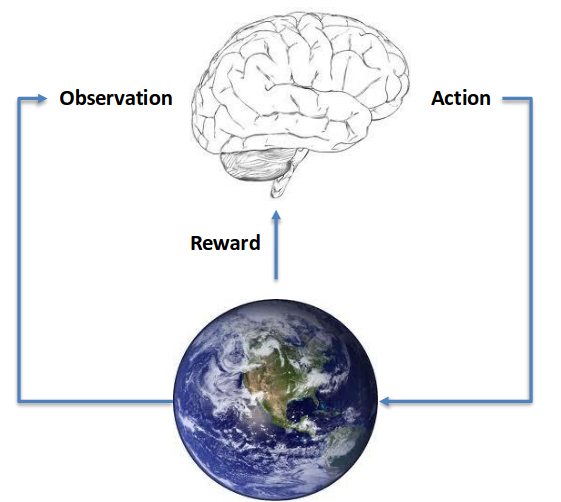
\includegraphics[width=0.5\textwidth]{images/AE.png}
    \caption{Interaction between agent and environment in reinforcement learning. At each time step $t$, the agent receives an observation $O_t$ and a scalar reward $R_t$, then executes an action $A_t$. The environment, in turn, receives the action $A_t$ and emits the next observation $O_{t+1}$ along with the reward $R_{t+1}$. The time index $t$ increments at each environment step, resulting in a continuous cycle of perception, action, and feedback that drives the agent's learning process.}
    \label{fig:rl_agent_environment}
\end{figure}

\section{History and State in Reinforcement Learning}

\subsection{The Role of History}
\begin{flushleft}
    The foundation of reinforcement learning dynamics lies in the concept of history, defined as the complete sequence of observations, actions, and rewards encountered by the agent up to any given time step. 
    \begin{equation}
    H_t = O_1, R_1, A_1, \ldots, A_{t-1}, O_t, R_t
    \end{equation}
    
    This history encompasses all observable variables that have occurred up to time $t$, creating a comprehensive record of the agent's interaction with its environment. The evolution of this history determines what happens next in the learning process, as both the agent's action selection and the environment's response depend fundamentally on this accumulated experience.
    
    The agent utilizes this historical information to select subsequent actions, while the environment processes the agent's actions to generate new observations and rewards. This creates a continuous cycle where past experiences inform future decisions, and future experiences expand the historical knowledge base available for decision-making.
\end{flushleft}

\subsection{State as a Function of History}
\begin{flushleft}
    While history provides complete information about past interactions, it quickly becomes unwieldy as the number of time steps increases. State emerges as a crucial abstraction that captures the essential information needed to determine future behavior. Formally, state is defined as a function of the history:
    $S_t = f(H_t)$.
    This functional relationship allows the agent to compress the potentially infinite sequence of past observations, actions, and rewards into a more manageable representation that retains the essential characteristics needed for decision-making. The choice of function $f$ becomes critical in determining how effectively the agent can learn and perform in its environment.
\end{flushleft}

\subsection{Environment State}
\begin{flushleft}
    The environment state $S_t^e$ represents the environment's private internal representation at time $t$. This encompasses whatever data the environment uses internally to determine the next observation and reward that will be provided to the agent. The environment state contains the complete information necessary for the environment to evolve according to its underlying dynamics.
    Typically, the environment state remains invisible to the agent, creating a fundamental information asymmetry in the learning process. Even when portions of the environment state become observable, they may contain substantial amounts of irrelevant information that do not directly influence the agent's decision-making process. This creates challenges in distinguishing between relevant and irrelevant environmental factors.
    The environment's internal representation often includes complex physical processes, hidden variables, and computational states that determine system behavior. In robotics applications, this might include precise motor positions, sensor calibrations, and physical dynamics that affect system response but remain hidden from the agent's direct observation.
\end{flushleft}

\subsection{Agent State}
\begin{flushleft}
    The agent state $S_t^a$ constitutes the agent's internal representation of the current situation, encompassing whatever information the agent uses to select its next action. This representation forms the foundation for all reinforcement learning algorithms, as it determines how the agent processes historical information and makes decisions.
    The agent state can be constructed as any function of the history:
    \begin{equation}
    S_t^a = f(H_t)
    \end{equation} This flexibility allows for diverse approaches to state representation, from simple memory-less strategies that only consider the current observation to sophisticated approaches that maintain complex internal models of environment dynamics.
    The quality of the agent state representation directly impacts learning performance and efficiency. Effective state representations capture relevant patterns in the environment while filtering out noise and irrelevant details. This balance between information retention and computational efficiency represents a key design consideration in reinforcement learning systems.
\end{flushleft}

\subsection{Information State and the Markov Property}
\begin{flushleft}
    An information state, also known as a Markov state, contains all useful information from the history necessary to predict future outcomes. A state $S_t$ satisfies the Markov property if and only if:
    \begin{equation}
         P[S_{t+1}|S_t] = P[S_{t+1}|S_1, \ldots, S_t]
    \end{equation}
    This mathematical condition captures the intuitive notion that "the future is independent of the past given the present." The Markov property creates a powerful simplification where the current state provides sufficient information to predict future behavior, allowing the entire history to be discarded once the state is known.
    The relationship can be visualized as: $H_{1:t} \rightarrow S_t \rightarrow H_{t+1:\infty}$, where the state $S_t$ acts as a sufficient statistic that captures all relevant information from the past history needed to predict future developments.     
    where the state $S_t$ acts as a sufficient statistic that captures all relevant information from the past history needed to predict future developments. This property proves essential for mathematical tractability in reinforcement learning algorithms.
    
    Both the environment state $S_t^e$ and the complete history $H_t$ naturally satisfy the Markov property. The environment state contains all information the environment uses for future evolution, while the history includes all possible relevant information by definition. However, constructing agent states that maintain the Markov property while remaining computationally tractable represents a central challenge in reinforcement learning.
\end{flushleft}

\section{Observability in Reinforcement Learning}

\subsection{Fully Observable Environments}
\begin{flushleft}
    Full observability occurs when the agent directly observes the complete environment state at each time step. In this scenario, the observation, agent state, and environment state become equivalent:
    \begin{equation}
    O_t = S_t^a = S_t^e
    \end{equation} This creates a transparent relationship between the agent's perception and the true state of the environment.
    Fully observable environments correspond formally to Markov Decision Processes (MDPs), which provide a mathematically tractable framework for reinforcement learning. The Markov property ensures that optimal decisions can be made based solely on current state information without requiring access to historical data.
    Examples of fully observable environments include many board games like chess or Go, where all relevant information remains visible to all players. Simple grid worlds and mathematical optimization problems also frequently satisfy full observability conditions, making them popular choices for developing and testing reinforcement learning algorithms.
\end{flushleft}

\subsection{Partially Observable Environments}
\begin{flushleft}
    Partial observability represents the more common and challenging scenario where agents indirectly observe the environment state through limited sensory information. In these situations, the agent state differs fundamentally from the environment state, creating information uncertainty that complicates decision-making.
    Real-world applications frequently involve partial observability. A robot navigating with camera vision lacks direct access to its precise global coordinates and must infer position from visual landmarks. Trading agents observe current market prices but cannot directly access the complete information driving market dynamics. Poker-playing agents see only public cards and their private hand while remaining unaware of opponents' cards and internal strategies.
    Partially observable environments correspond formally to Partially Observable Markov Decision Processes (POMDPs), which require more sophisticated solution techniques than standard MDPs. The agent must construct its own state representation $S_t^a$ that captures relevant information while managing uncertainty about hidden aspects of the environment.
    Several approaches exist for constructing agent states in partially observable environments. Complete history retention uses:
    \begin{equation}
    S_t^a = H_t
    \end{equation}
    maintaining all past information but potentially creating computational challenges as history length increases. Belief state approaches maintain probability distributions over possible environment states:
    \begin{equation}
    S_t^a = (P[S_t^e = s_1], \ldots, P[S_t^e = s_n])
    \end{equation}
    Modern approaches often employ recurrent neural networks to process sequential information:
    \begin{equation}
    S_t^a = \sigma(S_{t-1}^a W_s + O_t W_o)
    \end{equation}
    where $\sigma$ represents an activation function and $W_s, W_o$ are learned weight matrices.
    The choice of state representation strategy significantly impacts both learning efficiency and final performance in partially observable environments. Effective representations must balance information retention with computational tractability while adapting to the specific structure and dynamics of the target domain.
\end{flushleft}

\begin{figure}[H]
    \centering
    \begin{minipage}{0.45\textwidth}
        \centering
        
\includegraphics[width=\textwidth]{images/ex1.png}
        \label{fig:RL_Examples}
    \end{minipage}
    \hfill
    \begin{minipage}{0.4\textwidth}
        \centering
        
\includegraphics[width=\textwidth]{images/ex1_2.png}
        \label{fig:RL_Examples}
    \end{minipage}
    \label{fig:RL_Examples}
\end{figure}

\begin{flushleft}
    In the example above, the agent state is not a markov state, which means that the agent does not have access to all the information needed to make the best decision. The agent can only see what is around of it, and it cannot see what the whole map. This means that the agent cannot make the best decision because it does not have all the information it needs. In particulary the agent state in the two insighs position is the same,but the move to make is different.
\end{flushleft}

\section{Major Components of an RL Agent}

\begin{flushleft}
    A reinforcement learning agent may include one or more of the following fundamental components that define its architecture and capabilities. These components work together to enable the agent to perceive its environment, make decisions, and learn from experience. The specific combination and implementation of these components determine the agent's learning approach and performance characteristics.
\end{flushleft}

\subsection{Policy}
\begin{flushleft}
    A policy represents the agent's behavior function, serving as the core decision-making mechanism that maps from states to actions. The policy defines how the agent behaves at any given moment and constitutes the primary component that determines action selection in response to environmental observations.
    
    Given a state, the policy provides guidance on the best action or actions to take. This mapping can take different mathematical forms depending on the specific requirements and constraints of the learning problem.
    
    A deterministic policy provides a single action for each state:
    \begin{equation}
    a = \pi(s)
    \end{equation}
    where $\pi$ is the policy function that maps state $s$ directly to action $a$. This approach creates a clear, unambiguous decision rule but may lack the flexibility needed in uncertain environments.
    
    A stochastic policy defines a probability distribution over actions for each state:
    \begin{equation}
    \pi(a|s) = P[A_t = a | S_t = s]
    \end{equation}
    This formulation allows the agent to maintain uncertainty over action choices and enables exploration through probabilistic action selection. Stochastic policies prove particularly valuable in environments with incomplete information or when exploration is necessary for learning.
\end{flushleft}

\subsection{Value Function}
\begin{flushleft}
    The value function provides a prediction of future reward, serving as a mechanism to evaluate the goodness or badness of states and actions. This evaluation capability enables the agent to select actions based on their expected long-term consequences rather than immediate rewards.
    
    The state value function under policy $\pi$ is defined as:
    \begin{equation}
    v^\pi(s) = E[R_{t+1} + \gamma R_{t+2} + \gamma^2 R_{t+3} + \cdots | S_t = s]
    \end{equation}
    
    The discount factor $\gamma \in [0,1]$ controls the trade-off between immediate and long-term rewards. When $\gamma = 0$, the agent focuses entirely on immediate rewards, while $\gamma = 1$ weights all future rewards equally. Intermediate values create a preference for nearer rewards while still considering future consequences.
    
    Value functions serve multiple purposes in reinforcement learning. They enable the comparison of different states or actions based on their expected returns, provide a basis for policy improvement by identifying more valuable alternatives, and offer a mechanism for learning optimal behavior through value-based methods.
    
    Agents often approximate value functions when exact computation becomes intractable due to large state spaces or complex dynamics. Effective algorithms exist to learn these approximations efficiently, and with an accurate value function, agents can behave optimally. Even with suitable approximations, agents can achieve good performance in intractably large domains.
\end{flushleft}

\subsection{Model}
\begin{flushleft}
    A model predicts what the environment will do next, providing the agent with an internal representation of environmental dynamics. This predictive capability enables planning and forward-looking decision making, though it represents an optional component that not all reinforcement learning approaches require.
    
    The transition function $P$ predicts the next state given the current state and action:
    \begin{equation}
    P_{ss'}^a = P[S_{t+1} = s' | S_t = s, A_t = a]
    \end{equation}
    This probabilistic formulation captures the uncertainty inherent in many environments while providing expectations about state evolution.
    
    The reward function $R$ predicts the immediate reward expected from taking a specific action in a given state:
    \begin{equation}
    R_s^a = E[R_{t+1} | S_t = s, A_t = a]
    \end{equation}
    
    Together, these components create a complete model of environmental dynamics that can support various planning approaches. However, it's important to note that a model does not immediately provide a good policy. The agent must still engage in planning or other optimization processes to translate model predictions into effective action selection strategies.
    
    Model-based approaches offer several advantages including sample efficiency through simulated experience, the ability to reason about long-term consequences, and support for sophisticated planning algorithms. However, they also introduce challenges related to model accuracy, computational complexity, and the potential for model bias to negatively impact learning performance.
\end{flushleft}


\begin{figure}[H]
    \centering
    \begin{minipage}{0.3\textwidth}
        \centering
        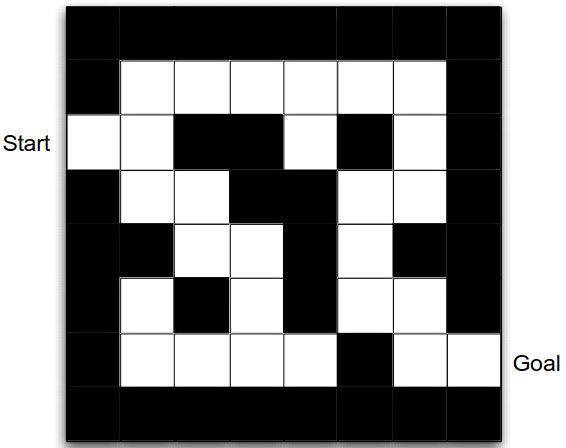
\includegraphics[width=\textwidth]{images/maze.png}
        \caption{Maze Examples}
        \label{fig:Maze_Examples}
    \end{minipage}
    \hfill
    \begin{minipage}{0.3\textwidth}
        \centering
        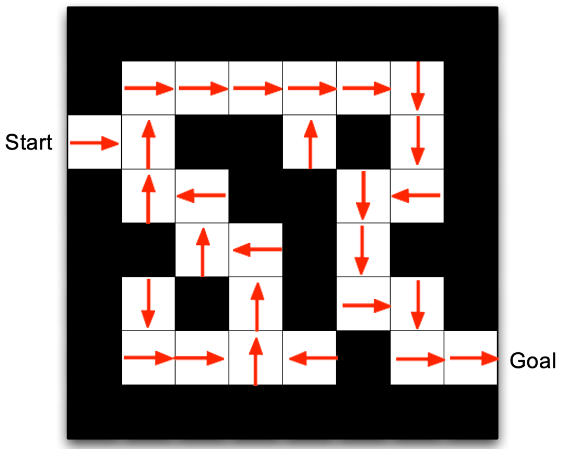
\includegraphics[width=\textwidth]{images/maze_policy.png}
        \caption{Maze Policy}
        \label{fig:Maze_Policy}
    \end{minipage}
    \label{fig:Maze_Examples}
\end{figure}


\begin{figure}[H]
    \centering
    \begin{minipage}{0.3\textwidth}
        \centering
        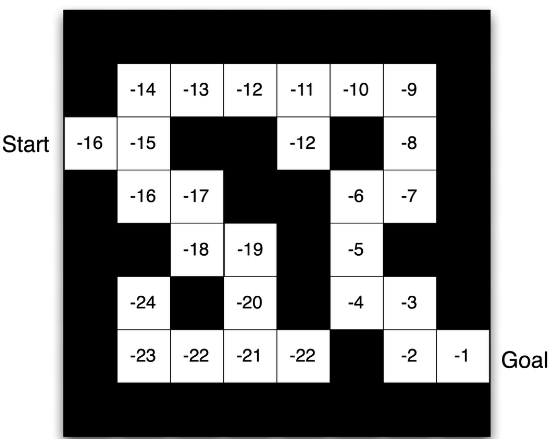
\includegraphics[width=\textwidth]{images/maze_value.png}
        \caption{Maze Value}
        \label{fig:Maze_Value}
    \end{minipage}
    \hfill
    \begin{minipage}{0.3\textwidth}
        \centering
        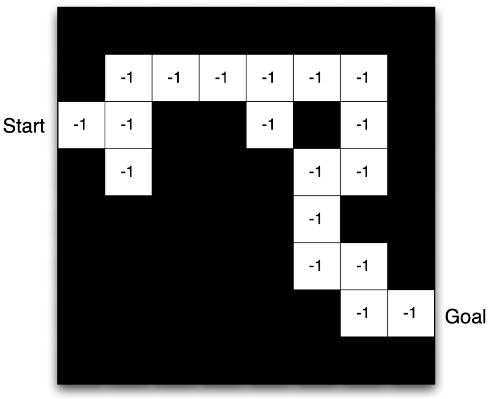
\includegraphics[width=\textwidth]{images/maze_model.png}
        \caption{Maze Model}
        \label{fig:Maze_Model}
    \end{minipage}
    \label{fig:Maze_model}
\end{figure}

\begin{flushleft}
    In the maze example above, reinforcement learning is illustrated through an agent that moves in the environment with four possible actions: north, east, south, and west, with its state corresponding to its position. Each step the agent takes incurs a penalty of -1, encouraging it to reach the goal in the fewest moves possible. The agent’s policy assigns an action to each state, represented by arrows in the cells, while the value function assigns a number to each state that reflects how advantageous it is to be there under the given policy. The agent may also build an internal model of the environment, describing how actions change the state and what rewards are received. This model, which represents the transition dynamics and the immediate rewards associated with states, can be imperfect or incomplete, but it helps guide decisions and predict the environment’s behavior.
\end{flushleft}

\section{Categorizing Reinforcement Learning Agents}

\begin{flushleft}
    Reinforcement learning agents can be systematically categorized based on their architectural components and learning approaches.
\end{flushleft}

\subsection{Component-Based Categorization}
\begin{flushleft}
    \textbf{Value-Based Agents} rely exclusively on value function estimation without maintaining an explicit policy representation. The policy emerges implicitly through greedy action selection from the value function.
    
    \textbf{Policy-Based Agents} maintain explicit policy representations without computing value functions, directly optimizing policy parameters to maximize expected returns.
    
    \textbf{Actor-Critic Agents} combine both policy and value function components. The critic estimates value functions while the actor maintains and updates the policy based on this feedback.
\end{flushleft}

\subsection{Model-Based vs Model-Free Categorization}
\begin{flushleft}
    \textbf{Model-Free Agents} learn directly from experience without constructing explicit models of environmental dynamics, reducing computational complexity but requiring more environmental interaction.
    
    \textbf{Model-Based Agents} construct internal models of environmental dynamics, enabling planning and achieving greater sample efficiency through simulated experience.
\end{flushleft}


\begin{figure}[H]
    \centering
    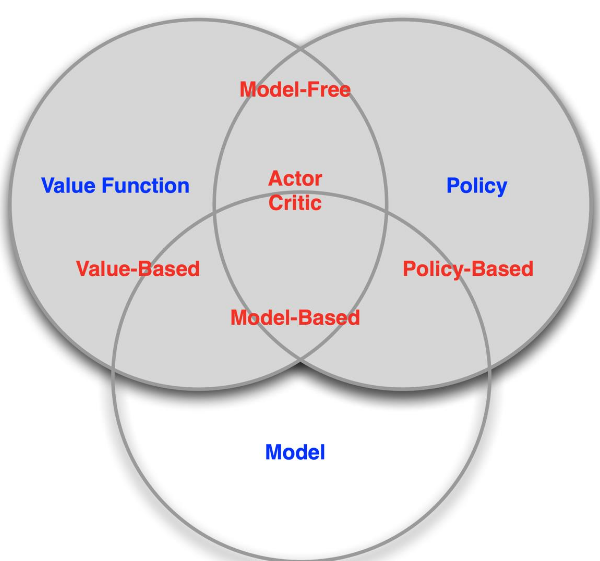
\includegraphics[width=0.4\textwidth]{images/RL_agent_taxonomy.png}
    \caption{Taxonomy of Reinforcement Learning Agents}
    \label{fig:RL_Agent_Taxonomy}
\end{figure}

\section{Learning and Planning in Reinforcement Learning}

\begin{flushleft}
    Sequential decision making encompasses two fundamental problem formulations that represent different approaches to optimizing agent behavior over time.
\end{flushleft}

\subsection{Reinforcement Learning}
\begin{flushleft}
    In reinforcement learning scenarios, the environment remains initially unknown to the agent. Learning occurs through direct interaction with the environment, where the agent observes states, executes actions, receives rewards, and uses this experience to improve its policy over time.
    
    This trial-and-error learning process requires the agent to balance exploration of unknown aspects of the environment with exploitation of current knowledge to maximize rewards. The agent must discover effective behaviors without access to optimal examples or complete environmental specifications.
    
    Real-world applications frequently exhibit these characteristics. Consider Atari game learning where the rules remain unknown initially. The agent must learn directly from interactive gameplay, selecting joystick actions and observing resulting pixels and scores. Through repeated interaction, the agent gradually discovers effective strategies without prior knowledge of game mechanics.
\end{flushleft}

\subsection{Planning}
\begin{flushleft}
    Planning scenarios assume complete knowledge of environmental dynamics through available models. The agent performs computational optimization using its model without requiring external environmental interaction during the planning phase. This enables the agent to simulate potential futures and optimize policies through internal computation.
    
    Planning approaches prove valuable when accurate models exist or can be constructed from limited data. In the Atari context, if complete game rules were known, the agent could query an internal emulator to determine the consequences of potential actions. This perfect model enables the agent to plan ahead using techniques such as tree search to identify optimal policies.
    
    The key distinction lies in information availability: reinforcement learning addresses unknown environments through interaction, while planning leverages known environmental models through computation.
\end{flushleft}

\section{Exploration and Exploitation}

\subsection{The Exploration-Exploitation Dilemma}
\begin{flushleft}
    Reinforcement learning resembles trial-and-error learning where agents must discover effective policies while minimizing reward loss during learning. The central challenge involves balancing exploration (gathering information about the environment) with exploitation (leveraging current knowledge to maximize rewards).
\end{flushleft}

\subsection{Examples}
\begin{flushleft}
    This trade-off appears across many domains: restaurant selection (favorite vs new restaurant), online advertising (successful vs experimental ads), and game playing (believed optimal vs exploratory moves).
\end{flushleft}

\section{Prediction and Control}

\begin{flushleft}
    Reinforcement learning problems naturally divide into two complementary categories that address different aspects of sequential decision making.
\end{flushleft}

\subsection{Prediction Problems}
\begin{flushleft}
    Prediction problems focus on evaluating future performance under given policies. The agent receives a specific policy and must determine its expected performance characteristics. This evaluation process requires estimating value functions that quantify long-term rewards achievable under the specified policy.
    
    Prediction serves multiple purposes including policy comparison, understanding environmental dynamics, and providing baselines for policy improvement algorithms. Accurate prediction capabilities enable agents to assess policy quality and identify areas for potential improvement.
\end{flushleft}


\begin{figure}[H]
    \centering
    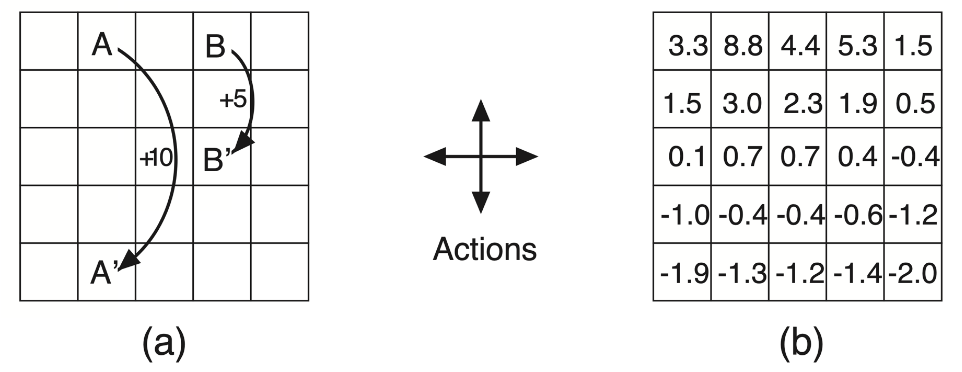
\includegraphics[width=0.5\textwidth]{images/prediction_ex.png}
    \caption{Prediction problem example}
    \label{fig:Prediction_Problem_Example}
\end{figure}


\subsection{Control Problems}
\begin{flushleft}
    Control problems address policy optimization without predetermined behavioral specifications. The agent must discover optimal policies through interaction and learning, combining prediction capabilities with policy improvement mechanisms.
    
    Control represents the ultimate goal of most reinforcement learning applications, where agents must autonomously discover effective behaviors. This requires sophisticated algorithms that can simultaneously evaluate current policies and identify improvements through exploration and value function updates.
\end{flushleft}


\begin{figure}[H]
    \centering
    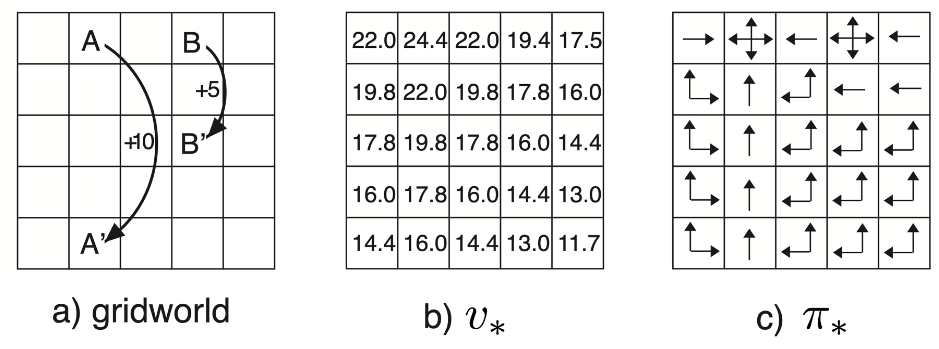
\includegraphics[width=0.5\textwidth]{images/controlo_ex.png}
    \caption{Control problem example}
    \label{fig:Control_Problem_Example}
\end{figure}


\section{Deep Reinforcement Learning}

\begin{flushleft}
    The integration of deep learning techniques with reinforcement learning creates powerful approaches for handling complex, high-dimensional problems that traditional methods cannot address effectively.
\end{flushleft}

\subsection{Function Approximation with Neural Networks}
\begin{flushleft}
    All major reinforcement learning components can be represented as functions suitable for neural network approximation.
    \begin{compactitemize}
        \item Policies map states to actions: $\pi: S \rightarrow A$. 
        \item Value functions map states to real-valued estimates: $v: S \rightarrow \mathbb{R}$. 
        \item Models map states to next states and rewards: $P: S \rightarrow S$ and $r: S \rightarrow \mathbb{R}$.    
    \end{compactitemize}
    Neural networks provide flexible function approximators capable of learning complex mappings from high-dimensional inputs. This enables reinforcement learning agents to handle image observations, continuous action spaces, and environments with millions of states.
\end{flushleft}

\subsection{Challenges in Deep Reinforcement Learning}
\begin{flushleft}
    Deep reinforcement learning violates fundamental assumptions underlying supervised learning approaches. The independent and identically distributed (i.i.d.) assumption fails because sequential decisions create correlated data where current actions influence future observations. Stationarity assumptions break down as the agent's changing policy modifies the data distribution over time.
    
    These violations require specialized techniques to ensure stable learning. Methods include experience replay to decorrelate training data, target networks to provide stable learning targets, and regularization approaches to handle non-stationary distributions. Successfully addressing these challenges enables deep reinforcement learning to achieve remarkable performance across diverse domains including game playing, robotics, and autonomous systems.
\end{flushleft}
\chapter{Markov Decision Process}

\section{Markov Processes}


Markov Decision Processes (MDPs) provide the formal mathematical framework for describing environments in reinforcement learning. This formalism captures the essential structure of sequential decision-making problems where an agent interacts with an environment over discrete time steps.

The fundamental assumption underlying MDPs is that the environment is fully observable, meaning the agent has complete access to all information necessary to understand the current state of the system. This complete observability ensures that the current state contains all relevant information needed to make optimal decisions and predict future outcomes.

The current state completely characterizes the process, embodying all the information from the history that is relevant for future decision-making. This property eliminates the need to maintain extensive historical records, as the present state provides sufficient information for optimal action selection.

The versatility of the MDP framework becomes apparent when considering that almost all reinforcement learning problems can be formalized as MDPs. Even scenarios that initially appear to violate MDP assumptions can often be transformed into the MDP framework. Partially observable problems can be converted into MDPs by expanding the state space to include belief states or by using recurrent neural networks to maintain internal memory. Bandit problems represent a special case of MDPs where only a single state exists, demonstrating the framework's broad applicability across different problem complexities.


\subsection{The Markov Property}


The central conceptual foundation of Markov Decision Processes rests on the Markov property, which embodies the principle that "the future is independent of the past, given the present." This fundamental assumption creates a mathematical structure that enables tractable solutions to complex sequential decision problems.

Formally, the Markov property is expressed as:
\begin{equation}
P[S_{t+1}|S_t] = P[S_{t+1}|S_1, \ldots, S_t]
\end{equation}

This equation captures the essence of the memoryless property: what happens next depends only on the current state, not on the sequence of events that led to the current situation. The entire history becomes irrelevant once the current state is known, as all relevant information is encapsulated within the present state.

The state $S_t$ represents a random variable that characterizes the agent's current position or situation within the environment. This state variable captures all the essential features of the environment that influence future transitions and rewards.

Critically, the state $S_t$ serves as a sufficient statistic of the future. This means that the current state contains all the information needed to predict future developments, making it unnecessary to consider the path taken to reach this state. This property dramatically simplifies both the mathematical analysis and computational implementation of learning algorithms, as it reduces the potentially infinite complexity of history-dependent decision making to a manageable state-based framework.


\subsection{State Transition Matrix}


The mathematical structure of Markov processes can be applied to any problem that satisfies the Markov property. The dynamics of state transitions are captured through transition probabilities that define how the system evolves over time.

For a Markov state $s$ and successor state $s'$, the state transition probability is defined by:
\begin{equation}
\mathcal{P}_{ss'} = \mathbb{P}[S_{t+1} = s' | S_t = s]
\end{equation}

This probability quantifies the likelihood of transitioning from state $s$ to state $s'$ in a single time step, providing a complete specification of the system's stochastic dynamics.

Given a current state $s$, the state transition matrix defines the probability distribution over all possible next states $s'$. This matrix representation provides a comprehensive characterization of the environment's dynamics and defines the complete structure of the Markov problem.

The state transition matrix $\mathcal{P}$ takes the form:
\begin{equation}
\mathcal{P} = \begin{pmatrix}
\mathcal{P}_{11} & \cdots & \mathcal{P}_{1n} \\
\vdots & \ddots & \vdots \\
\mathcal{P}_{n1} & \cdots & \mathcal{P}_{nn}
\end{pmatrix}
\end{equation}

Each row of this matrix corresponds to a current state, while each column represents a possible next state. The entry $\mathcal{P}_{ij}$ specifies the probability of transitioning from state $i$ to state $j$. Since these represent probability distributions, each row sums to one, ensuring that the system must transition to some next state with certainty.

This matrix representation enables efficient computation of multi-step transition probabilities through matrix multiplication, facilitates analysis of long-term system behavior, and provides the foundation for value iteration and policy evaluation algorithms in reinforcement learning.


\subsection{Markov Process}


A Markov process represents a memoryless random process, consisting of a sequence of random states $S_1, S_2, \ldots$ that satisfy the Markov property. This mathematical construct provides the foundation for understanding stochastic systems where future evolution depends only on the current state.

Formally, a Markov process is defined as a tuple $\langle \mathcal{S}, \mathcal{P} \rangle$, where:
\begin{compactitemize}
\item $\mathcal{S}$ is a finite set of states representing all possible configurations of the system
\item $\mathcal{P}$ is a state transition probability matrix where $\mathcal{P}_{ss'} = \mathbb{P}[S_{t+1} = s' | S_t = s]$
\end{compactitemize}

At this level of abstraction, the process includes no actions, meaning there is no decision-maker influencing the system's evolution. The system transitions between states according to the fixed probabilities specified in the transition matrix, without any external control or intervention.

Similarly, no rewards are present in a basic Markov process. The system simply evolves through its state space without any notion of desirable or undesirable outcomes. This represents the simplest form of stochastic process that maintains the Markov property.

Despite these limitations, Markov processes provide crucial insights into system dynamics and serve as building blocks for more complex formulations that incorporate decision-making and reward structures. Understanding Markov processes enables the development of intuition about state-based systems and provides the mathematical foundation for Markov Decision Processes.


\subsection{Example: Student Markov Chain}


To illustrate the concepts of Markov processes, consider a student's daily activity patterns modeled as a Markov chain. This example demonstrates how real-world scenarios can be abstracted into mathematical frameworks while maintaining essential behavioral characteristics.

The student's possible states include:
\begin{compactitemize}
\item Class 1, Class 2, Class 3: Different academic activities
\item Pass: Successfully completing coursework
\item Pub: Social activities
\item TikTok: Social media engagement
\item Sleep: Rest periods
\end{compactitemize}

The transition probabilities capture realistic behavioral patterns, and there are show below with the example scheme.



\begin{figure}[H]
    \centering
    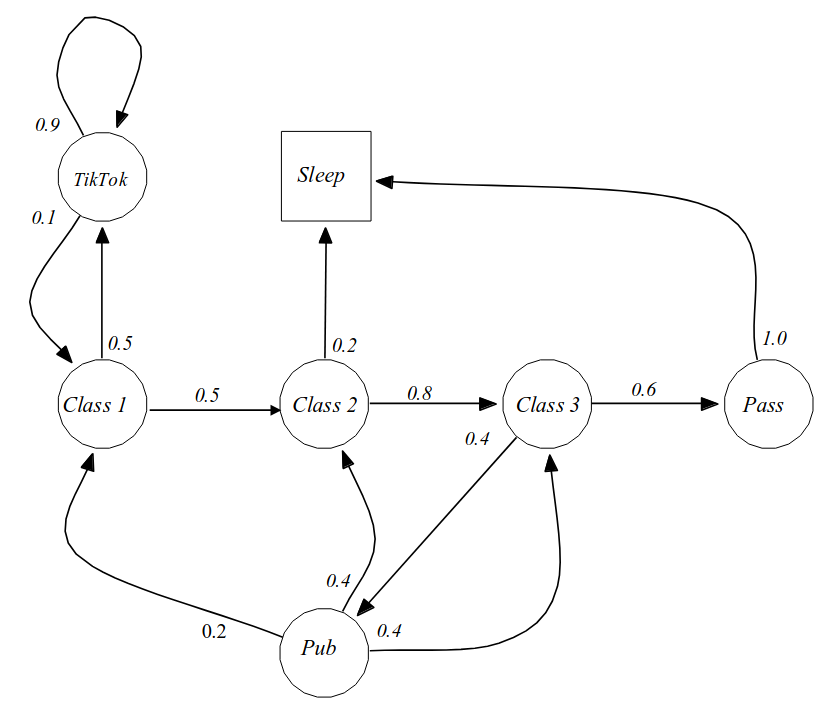
\includegraphics[width=0.6\textwidth]{images/student_chain.png}
    \caption{Student Markov Chain illustrating states and transition probabilities.}
    \label{fig:student_markov_chain}
\end{figure}

\subsubsection{Sample Episodes}

Sampling from this Markov chain generates random sequences of variable length that reflect the stochastic nature of student behavior. Each sample represents a possible trajectory through the state space, determined by the transition probabilities.

Example episodes include:
\begin{compactitemize}
\item C1 → C2 → C3 → Pass → Sleep
\item C1 → TK → TK → C1 → C2 → Sleep  
\item C1 → TK → TK → C1 → C2 → C3 → Pub → C1 → TK → TK → TK → C1 → C2 → C3 → Pub → C2 → Sleep
\end{compactitemize}

These episodes demonstrate several important characteristics of Markov processes. The first episode shows an ideal progression through all class states to successful completion. The second episode illustrates how distractions (TikTok) can interrupt but not necessarily prevent eventual progress. The third episode reveals the complex, potentially lengthy paths that can result from repeated cycles between productive and unproductive states.

The variable length of these episodes reflects the stochastic nature of the process and the presence of absorbing states that terminate the sequence. This variability captures the uncertainty inherent in modeling complex behavioral systems while maintaining the mathematical tractability provided by the Markov property.


\subsubsection{Transition Matrix Representation}

The complete dynamics of the Student Markov Chain can be represented in matrix form, providing a comprehensive specification of all possible state transitions and their associated probabilities.

\begin{equation}
\mathcal{P} = \begin{array}{c|ccccccc}
 & C1 & C2 & C3 & Pass & Pub & TK & Sleep \\
\hline
C1 & 0 & 0.5 & 0 & 0 & 0 & 0.5 & 0 \\
C2 & 0 & 0 & 0.8 & 0 & 0.4 & 0 & 0.2 \\
C3 & 0 & 0 & 0 & 0.6 & 0.4 & 0 & 0 \\
Pass & 0 & 0 & 0 & 0 & 0 & 0 & 1.0 \\
Pub & 0.2 & 0 & 0 & 0 & 0.4 & 0 & 0.4 \\
TK & 0.1 & 0 & 0 & 0 & 0 & 0.9 & 0 \\
Sleep & 0 & 0 & 0 & 0 & 0 & 0 & 1.0
\end{array}
\end{equation}

This matrix representation reveals several important structural properties. Each row represents a current state and sums to 1.0, ensuring that transition probabilities form valid probability distributions. The diagonal elements show self-transition probabilities, with high values for TikTok (0.9) indicating strong tendency to remain distracted, and values of 1.0 for Pass and Sleep indicating absorbing states.

The sparsity of the matrix reflects the realistic constraint that not all state transitions are possible or likely. For example, there are no direct transitions from Sleep to active states, and the Pass state only transitions to Sleep, representing the natural conclusion of academic activities.

This matrix enables computation of long-term behavior through matrix powers, analysis of steady-state distributions, and calculation of expected hitting times between states. Such analyses provide insights into the long-term consequences of different behavioral patterns and the overall structure of the system dynamics.


\section{Markov Reward Process}


A Markov Reward Process (MRP) extends the concept of a Markov Process by associating a reward with each state. This framework introduces the notion of value, allowing us to evaluate the desirability of states in terms of expected future rewards.

Formally, an MRP is defined as a tuple $\langle \mathcal{S}, \mathcal{P}, \mathcal{R}, \gamma \rangle$, where:
\begin{itemize}
    \item $\mathcal{S}$ is a finite set of states
    \item $\mathcal{P}$ is the state transition probability matrix
    \item $\mathcal{R}$ is a reward function, where $\mathcal{R}_s = \mathbb{E}[R_{t+1} | S_t = s]$
    \item $\gamma$ is a discount factor, $\gamma \in [0,1]$, representing the present value of future rewards
\end{itemize}

The total return from a state $S_t$ is defined as the discounted sum of future rewards:
\begin{equation}
G_t = R_{t+1} + \gamma R_{t+2} + \gamma^2 R_{t+3} + \cdots
= \sum_{k=0}^{\infty} \gamma^k R_{t+k+1}
\end{equation}

The \textbf{state-value function} $v(s)$ represents the expected return starting from state $s$:
\begin{equation}
v(s) = \mathbb{E}[G_t \mid S_t = s] 
= \mathbb{E}[R_{t+1} + \gamma v(S_{t+1}) \mid S_t = s]
\end{equation}

\begin{figure}[H]
    \centering
    \begin{minipage}{0.45\textwidth}
        \centering
        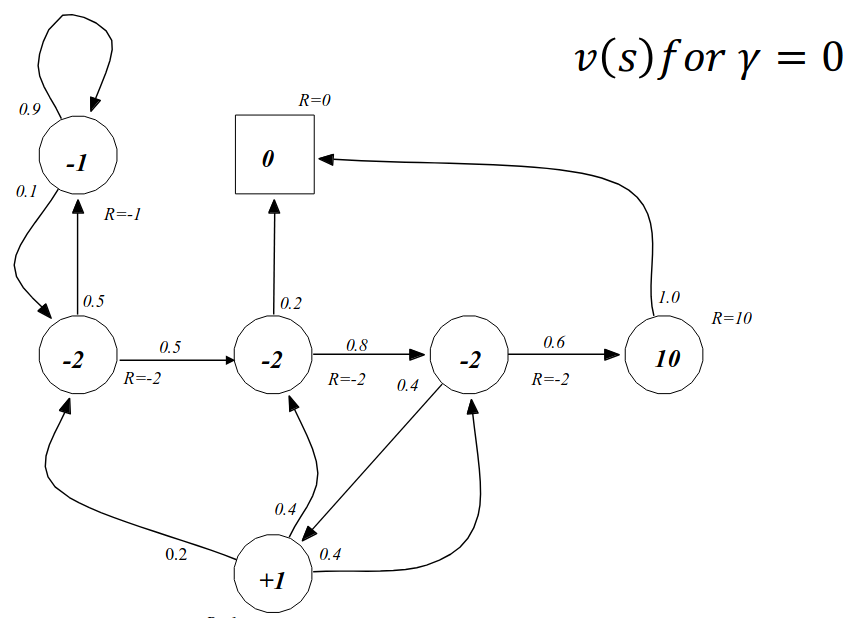
\includegraphics[width=\textwidth]{images/gamm0.png}
        \caption{Student Markov Chain with $\gamma=0$}
        \label{fig:STMCR}
    \end{minipage}
    \hfill
    \begin{minipage}{0.45\textwidth}
        \centering
        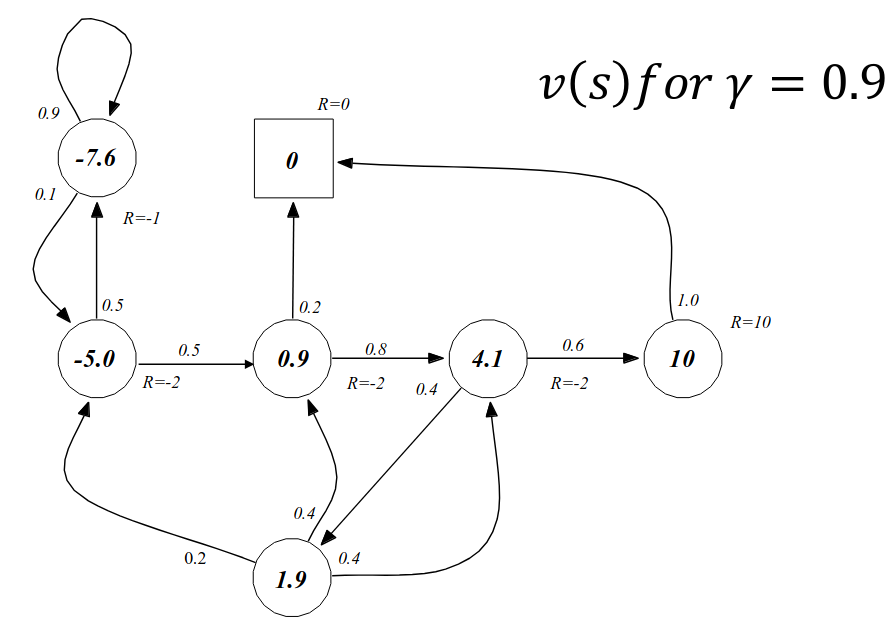
\includegraphics[width=\textwidth]{images/gamma9.png}
        \caption{Student Markov Chain with $\gamma=0.9$}
        \label{fig:STMCR}
    \end{minipage}
    \label{STMCR}
\end{figure}

\subsection{Bellman Equation for MRPs}

The fundamental idea behind the Bellman equation for Markov Reward Processes is that the value function admits a \textbf{recursive decomposition}. The value of a state does not depend directly on the entire future sequence of rewards, but can be expressed as the sum of two contributions: the immediate reward and the expected value of the next state, appropriately discounted.

By definition, the value function of a state $s$ is the expected value of the return starting from that state:
\[
v(s) = \mathbb{E}\!\left[ G_t \mid S_t = s \right]
\]
where the return is defined as:
\[
G_t = R_{t+1} + \gamma R_{t+2} + \gamma^2 R_{t+3} + \dots
\]

Making this definition explicit, we obtain:
\[
v(s)
=
\mathbb{E}
\left[
R_{t+1}
+ \gamma R_{t+2}
+ \gamma^2 R_{t+3}
+ \dots
\;\middle|\;
S_t = s
\right]
\]

Grouping the first term and factoring out $\gamma$, the return can be rewritten as:
\[
v(s)
=
\mathbb{E}
\left[
R_{t+1}
+ \gamma
\left(
R_{t+2}
+ \gamma R_{t+3}
+ \dots
\right)
\;\middle|\;
S_t = s
\right]
\]

Observing that the expression in parentheses coincides with the return starting from time $t+1$, we obtain:
\[
v(s)
=
\mathbb{E}
\left[
R_{t+1}
+ \gamma G_{t+1}
\;\middle|\;
S_t = s
\right]
\]

Since $G_{t+1}$ is, by definition, the return starting from state $S_{t+1}$, the term can be expressed as the value function of the next state:
\[
v(s)
=
\mathbb{E}
\left[
R_{t+1}
+ \gamma v(S_{t+1})
\;\middle|\;
S_t = s
\right]
\]

This equation compactly expresses the principle according to which the overall value of a state is given by the expected immediate reward plus the discounted value of the next state.

In the case of a Markov Reward Process, the expected reward and the transition probabilities depend only on the current state. Denoting by $\mathcal{R}_s$ the average reward associated with state $s$ and by $\mathcal{P}_{ss'}$ the transition probability from $s$ to $s'$, the expectation can be made explicit:
\[
v(s)
=
\mathcal{R}_s
+
\gamma
\sum_{s' \in \mathcal{S}}
\mathcal{P}_{ss'} \, v(s')
\]

This is the \textbf{Bellman equation for Markov Reward Processes}. It provides a recursive characterization of the value function and is the theoretical foundation of all prediction and control algorithms in Reinforcement Learning.

\subsection{Matrix Form}


In matrix notation, the Bellman equation is:
\begin{equation}
v = \mathcal{R} + \gamma \mathcal{P} v \quad \Rightarrow \quad v = (I - \gamma \mathcal{P})^{-1} \mathcal{R}
\end{equation}

For example, consider a small MRP with 3 states:
\[
\mathcal{P} =
\begin{bmatrix}
0.5 & 0.2 & 0.3 \\
0.1 & 0.9 & 0.0 \\
0.4 & 0.4 & 0.2
\end{bmatrix}, \quad
\mathcal{R} =
\begin{bmatrix}
-1 \\
10 \\
0
\end{bmatrix}, \quad \gamma = 1
\]

The value vector $v$ can be computed as:
\[
v =
\begin{bmatrix}
v_1 \\
v_2 \\
v_3
\end{bmatrix} =
\mathcal{R} + \gamma \mathcal{P} v
=
\begin{bmatrix}
-1 \\
10 \\
0
\end{bmatrix} +
\begin{bmatrix}
0.5 & 0.2 & 0.3 \\
0.1 & 0.9 & 0.0 \\
0.4 & 0.4 & 0.2
\end{bmatrix}
\begin{bmatrix}
v_1 \\
v_2 \\
v_3
\end{bmatrix}
\]



This illustrates how the Bellman equation can be written in matrix form, which is particularly useful for computational solutions of MRPs. The computation complexity is $O(n^3)$ due to the matrix inversion, where $n$ is the number of states. Direct solution is possible only for small MRPs.
There are many iterative methods for latge MRPs,such as:
\begin{compactitemize}
    \item Dynamic Programming
    \item Monte-Carlo methods
    \item Temporal-Difference Learning
\end{compactitemize}


\section{Markov Decision Process}


While Markov Reward Processes provide a framework for evaluating states in terms of expected rewards, they lack the crucial element of agency. In MRPs, the agent has no control over the system's evolution and simply flows through the environment according to the fixed transition probabilities specified in $\mathcal{P}$. This limitation necessitates the introduction of decision-making capabilities.

A Markov Decision Process (MDP) extends the MRP framework by incorporating actions and decision-making, creating an environment where an agent can influence the system's evolution through deliberate choices. MDPs represent the mathematical foundation for sequential decision-making under uncertainty, where all states maintain the Markov property.

Formally, an MDP is defined as a tuple $\langle \mathcal{S}, \mathcal{A}, \mathcal{P}, \mathcal{R}, \gamma \rangle$, where:
\begin{compactitemize}
\item $\mathcal{S}$ is a finite set of states representing all possible configurations of the environment
\item $\mathcal{A}$ is a finite set of actions available to the agent
\item $\mathcal{P}$ is a state transition probability matrix, where $\mathcal{P}_{ss'}^a = \mathbb{P}[S_{t+1} = s' | S_t = s, A_t = a]$
\item $\mathcal{R}$ is a reward function, where $\mathcal{R}_s^a = \mathbb{E}[R_{t+1} | S_t = s, A_t = a]$
\item $\gamma$ is a discount factor, $\gamma \in [0,1]$
\end{compactitemize}

The critical distinction from MRPs lies in the action-dependent nature of both transitions and rewards. The probability of transitioning to state $s'$ now depends not only on the current state $s$ but also on the action $a$ chosen by the agent. Similarly, the expected reward depends on both the current state and the selected action, providing the agent with the ability to influence both immediate rewards and future state evolution.



\begin{figure}[H]
    \centering
    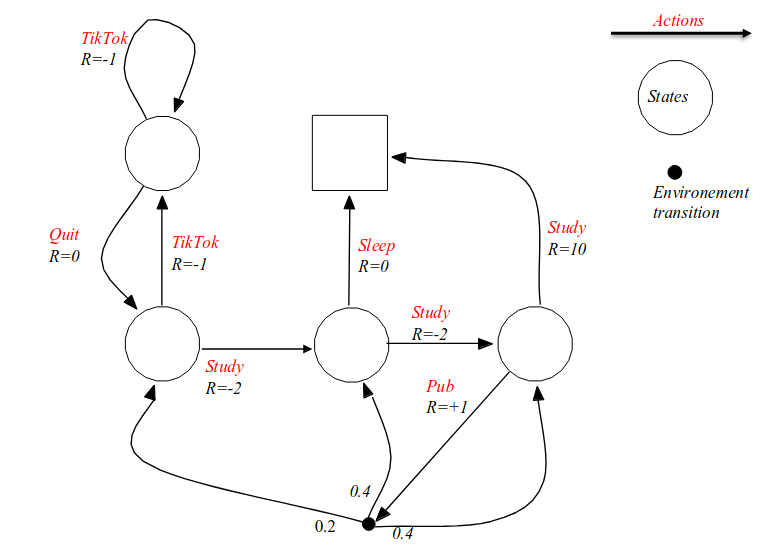
\includegraphics[width=0.6\textwidth]{images/MDP_chain.png}
    \caption{Student MDP Chain.}
    \label{fig:student_markov_chain}
\end{figure}


    \textbf{Note:}The black point in the figure above rappresent an enviroment transition, this is not under the control of the agent. So with a some probability the agent will move to one of the possible next states.


\subsection{Policy}


The concept of agency in MDPs is formalized through the notion of a policy, which defines how an agent behaves in the environment. A policy serves as the decision-making mechanism that maps states to actions, providing a complete specification of the agent's behavior strategy.

A policy $\pi$ is formally defined as a distribution over actions given states:
\begin{equation}
\pi(a|s) = \mathbb{P}[A_t = a | S_t = s]
\end{equation}

This probabilistic formulation allows for both deterministic policies, where a single action is chosen with probability 1, and stochastic policies, where actions are selected according to a probability distribution. The policy completely defines the agent's behavior, as it specifies how the agent chooses actions based solely on the current state.

Several important properties characterize MDP policies. First, policies depend only on the current state, not on the history of states, actions, or rewards. This memoryless property aligns with the Markov assumption and ensures that optimal decision-making requires only knowledge of the present situation.

Second, policies focus exclusively on future rewards, disregarding past experiences in the decision-making process. This forward-looking perspective reflects the goal-oriented nature of reinforcement learning, where the objective is to maximize expected future returns rather than to optimize past performance.

Finally, policies are stationary, meaning they are time-independent. The same policy applies regardless of when a decision is made, providing consistency across different time steps and enabling the development of stable behavioral strategies.


\subsection{Value Functions}


Value functions provide the mathematical foundation for evaluating the quality of states and actions under a given policy. These functions quantify the expected future performance of different choices, enabling rational decision-making in uncertain environments.

The \textbf{state-value function} $v^\pi(s)$ represents the expected return when starting from state $s$ and subsequently following policy $\pi$:
\begin{equation}
v_\pi(s) = \mathbb{E}_\pi[G_t | S_t = s]
\end{equation}

This function captures the long-term value of being in a particular state under a specific policy, incorporating both immediate rewards and the discounted value of all future states that may be visited.

The \textbf{action-value function} $q^\pi(s,a)$ extends this concept by evaluating the expected return when starting from state $s$, taking action $a$, and then following policy $\pi$:
\begin{equation}
q_\pi(s,a) = \mathbb{E}_\pi[G_t | S_t = s, A_t = a]
\end{equation}

The action-value function provides more granular information by distinguishing between the values of different actions in the same state. This additional detail enables the comparison of alternative actions and supports the development of improved policies through action selection based on expected returns.

These value functions form the basis for policy evaluation, policy improvement, and ultimately the discovery of optimal policies that maximize expected returns across all states and situations.

\subsubsection{Bellman Equations for MDPs}

In Markov Decision Processes too, the value function admits a recursive decomposition, analogous to that of Markov Reward Processes, with the fundamental difference that the dynamics of the environment now also depend on the actions selected according to a policy $\pi$.

Consider a fixed policy $\pi$. The state-value function $v_\pi(s)$ is defined as the expected return starting from state $s$ and following the policy $\pi$:
\[
v_\pi(s) = \mathbb{E}_\pi \big[ G_t \mid S_t = s \big]
\]

Using the definition of return and separating the first term, the value of the state can be expressed as:
\[
v_\pi(s)
=
\mathbb{E}_\pi
\big[
R_{t+1} + \gamma G_{t+1}
\mid S_t = s
\big]
\]

Since $G_{t+1}$ represents the return starting from the next state $S_{t+1}$, we obtain the first form of the Bellman expectation equation:
\[
v_\pi(s)
=
\mathbb{E}_\pi
\big[
R_{t+1} + \gamma v_\pi(S_{t+1})
\mid S_t = s
\big]
\]

In a completely analogous way, it is possible to obtain a recursive decomposition for the action-value function. The function $q_\pi(s,a)$ represents the expected return starting from state $s$, executing action $a$ and then following the policy $\pi$:
\[
q_\pi(s,a)
=
\mathbb{E}_\pi
\big[
R_{t+1} + \gamma q_\pi(S_{t+1}, A_{t+1})
\mid S_t = s, A_t = a
\big]
\]

These relations express the general principle according to which the expected value is given by the immediate reward plus the expected value of the next step.

To make the equations completely explicit, the expectation operator can be eliminated by introducing the policy $\pi$, the reward function $\mathcal{R}$ and the transition probabilities $\mathcal{P}$. The state-value function can be rewritten as a weighted average of the action-value functions:
\[
v_\pi(s) = \sum_{a \in \mathcal{A}} \pi(a \mid s)\, q_\pi(s,a)
\]

In turn, the action-value function satisfies:
\[
q_\pi(s,a)
=
\mathcal{R}_s^a
+
\gamma
\sum_{s' \in \mathcal{S}}
\mathcal{P}_{ss'}^a \, v_\pi(s')
\]

Substituting this expression into the definition of $v_\pi(s)$, we obtain the Bellman expectation equation for the state-value function:
\[
v_\pi(s)
=
\sum_{a \in \mathcal{A}}
\pi(a \mid s)
\left[
\mathcal{R}_s^a
+
\gamma
\sum_{s' \in \mathcal{S}}
\mathcal{P}_{ss'}^a
\, v_\pi(s')
\right]
\]

Analogously, substituting the definition of $v_\pi(s')$ in terms of $q_\pi$, we obtain the Bellman expectation equation for the action-value function:
\[
q_\pi(s,a)
=
\mathcal{R}_s^a
+
\gamma
\sum_{s' \in \mathcal{S}}
\mathcal{P}_{ss'}^a
\sum_{a' \in \mathcal{A}}
\pi(a' \mid s')\, q_\pi(s',a')
\]

These equations completely characterize the evaluation of a policy in an MDP and are the theoretical basis of all policy evaluation algorithms, both model-based and model-free. In particular, they show how the effect of future actions is incorporated into the value through the expectation with respect to the policy $\pi$.

\subsection{Optimal Value Functions}

In a Markov Decision Process, the goal of the control problem is to determine the best performance achievable by the agent over all states. This information is captured by the \textbf{optimal value functions}.

The \textbf{optimal state-value function} is defined as the maximum value achievable starting from state $s$ over all possible policies:
\[
v^*(s) = \max_{\pi} v_\pi(s)
\]

Analogously, the \textbf{optimal action-value function} is defined as the maximum value achievable starting from the state–action pair $(s,a)$ over all policies:
\[
q^*(s,a) = \max_{\pi} q_\pi(s,a)
\]

The optimal value function therefore represents the upper bound of the performance achievable in an MDP. An MDP is said to be \emph{solved} when the optimal value function is known, since an optimal policy can be derived directly from it.
\begin{figure}[H]
    \centering
    \begin{minipage}{0.45\textwidth}
        \centering
        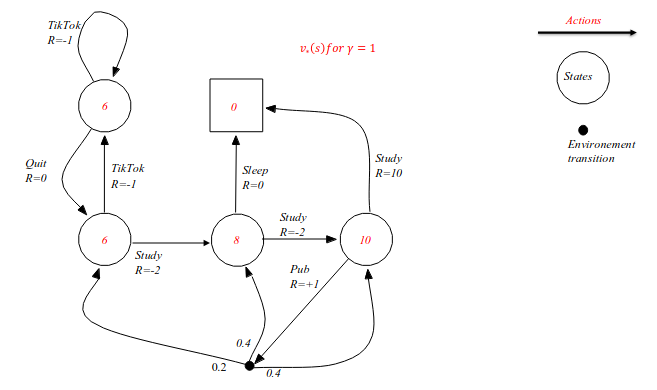
\includegraphics[width=\textwidth]{images/L11.png}
        \caption{Optimal value function for student MDP}
        \label{fig:STMCR}
    \end{minipage}
    \hfill
    \begin{minipage}{0.45\textwidth}
        \centering
        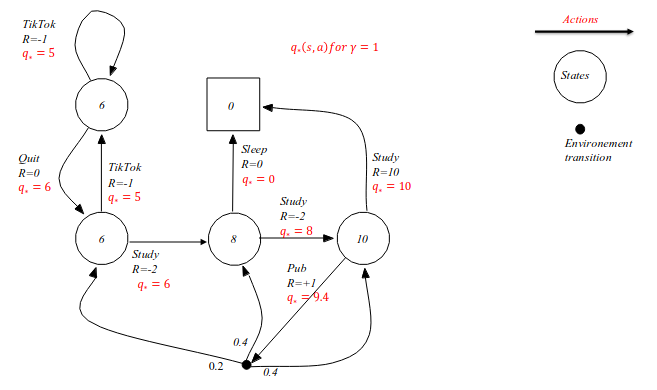
\includegraphics[width=\textwidth]{images/L12.png}
        \caption{Optimal action-value function for Studenr MDP}
        \label{fig:STMCR}
    \end{minipage}
    \label{STMCR}
\end{figure}


\subsection{Optimal Policies}

It is possible to introduce a partial ordering between policies by comparing their respective state values. Given two policies $\pi$ and $\pi'$, we say that:
\[
\pi \ge \pi'
\quad \text{if and only if} \quad
v_\pi(s) \ge v_{\pi'}(s) \quad \forall s \in \mathcal{S}
\]

A fundamental result of Reinforcement Learning states that, for every MDP, \textbf{there exists at least one optimal policy} $\pi^*$ such that:
\[
\pi^* \ge \pi \qquad \forall \pi
\]

All optimal policies share the same optimal value functions:
\[
v_{\pi^*}(s) = v^*(s),
\qquad
q_{\pi^*}(s,a) = q^*(s,a)
\]

A particularly important fact is that, for every MDP, \textbf{there always exists a deterministic optimal policy}. This means that it is not necessary to resort to randomization to obtain optimal behaviour.

If the optimal action-value function is known, an optimal policy can be obtained directly by choosing, in every state, the action that maximizes $q^*(s,a)$:
\[
\pi^*(a \mid s) =
\begin{cases}
1 & \text{if } a \in \arg\max_{a' \in \mathcal{A}} q^*(s,a') \\
0 & \text{otherwise}
\end{cases}
\]

This relation shows that knowing $q^*$ is sufficient to completely determine an optimal policy.


\subsection{Bellman Optimality Equations}

The optimal value functions satisfy a recursive relation called the \textbf{Bellman optimality equation}. Unlike the Bellman expectation equations, in this case the expectation with respect to the policy is replaced by a maximum operation, since the agent is assumed to act optimally.

The Bellman optimality equation for the state-value function is:
\[
v^*(s) = \max_{a \in \mathcal{A}} q^*(s,a)
\]

Explicitly expressing the dynamics of the MDP, the same equation can be written as:
\[
v^*(s)
=
\max_{a \in \mathcal{A}}
\left[
\mathcal{R}_s^a
+
\gamma
\sum_{s' \in \mathcal{S}}
\mathcal{P}_{ss'}^a \, v^*(s')
\right]
\]

Analogously, the Bellman optimality equation for the action-value function is:
\[
q^*(s,a)
=
\mathcal{R}_s^a
+
\gamma
\sum_{s' \in \mathcal{S}}
\mathcal{P}_{ss'}^a
\max_{a' \in \mathcal{A}} q^*(s',a')
\]

These equations completely characterize the control problem in Markov Decision Processes. The functions $v^*$ and $q^*$ are the fixed points of these Bellman operators and are the theoretical foundation of all control algorithms, both model-based and model-free, such as Value Iteration, Policy Iteration, SARSA and Q-learning.

\chapter{Planning by Dynamic Programming}

\section{Introduction}

La Dynamic Programming (DP) è un insieme di metodi utilizzati per risolvere problemi decisionali caratterizzati da una struttura sequenziale o temporale. Il termine \emph{dynamic} indica che il problema evolve nel tempo, mentre \emph{programming} non si riferisce alla programmazione software, bensì all’ottimizzazione di un programma decisionale, ovvero di una policy.

La Dynamic Programming fornisce un approccio generale per affrontare problemi complessi, suddividendoli in sottoproblemi più semplici. Risolvendo questi sottoproblemi e combinandone le soluzioni, è possibile ottenere una soluzione ottimale per il problema originale. Questo approccio è particolarmente efficace quando gli stessi sottoproblemi si presentano ripetutamente durante il processo di risoluzione.

Nel contesto del Reinforcement Learning, la Dynamic Programming viene utilizzata come metodo di \emph{planning}, cioè come tecnica che assume la conoscenza completa del modello dell’ambiente e consente di calcolare policy e value function senza interagire con l’ambiente.


\subsection{Requirements for Dynamic Programming}

La Dynamic Programming è applicabile solo a problemi che soddisfano due proprietà fondamentali. La prima è la presenza di una struttura di \emph{optimal substructure}, formalizzata dal principio di ottimalità. Questo principio afferma che una policy ottimale ha la proprietà che, per qualsiasi stato iniziale, le azioni successive devono costituire una policy ottimale per il sottoproblema indotto dallo stato successivo. Di conseguenza, una soluzione ottimale globale può essere costruita a partire da soluzioni ottimali di sottoproblemi più piccoli.

La seconda proprietà è la presenza di \emph{overlapping subproblems}. Durante la risoluzione del problema, gli stessi sottoproblemi compaiono più volte, rendendo possibile memorizzarne le soluzioni e riutilizzarle. Questo meccanismo permette di ridurre significativamente il costo computazionale.

I Markov Decision Processes soddisfano naturalmente entrambe queste proprietà. In particolare, la dinamica markoviana garantisce la validità del principio di ottimalità, mentre la Bellman equation fornisce una decomposizione ricorsiva del problema. La value function rappresenta il mezzo attraverso il quale le soluzioni dei sottoproblemi vengono archiviate e riutilizzate.


\subsection{Planning for Dynamic Programming}

La Dynamic Programming assume una conoscenza completa dell’MDP, ovvero dell’insieme degli stati $\mathcal{S}$, dell’insieme delle azioni $\mathcal{A}$, della funzione di transizione $P$, della reward function $R$ e del fattore di sconto $\gamma$. In questo contesto, la DP viene utilizzata per svolgere attività di planning.

Nel problema di \emph{prediction}, l’obiettivo è valutare una policy fissata $\pi$. L’input è un MDP descritto dalla tupla
\[
\langle \mathcal{S}, \mathcal{A}, P, R, \gamma \rangle
\]
insieme alla policy $\pi$, mentre l’output è la corrispondente value function $v^\pi$.

Nel problema di \emph{control}, invece, l’obiettivo è determinare la policy ottimale. In questo caso l’input è solo l’MDP e l’output consiste nella value function ottimale $v^*$ e nella policy ottimale $\pi^*$.

In entrambi i casi, la Dynamic Programming utilizza le Bellman equations per propagare l’informazione sugli stati e ottenere soluzioni sempre più accurate tramite aggiornamenti iterativi.


\section{Iterative Policy Evaluation}

L'Iterative Policy Evaluation calcola la value function $v^\pi$ di una policy fissata $\pi$ applicando in modo iterativo la Bellman expectation equation. Ad ogni iterazione $k+1$ si aggiorna il valore di ogni stato $s \in \mathcal{S}$ secondo:

\[
v_{k+1}(s) \;=\; \sum_{a \in \mathcal{A}} \pi(a \mid s) 
\Bigg( R_s^a \;+\; \gamma \sum_{s' \in \mathcal{S}} P_{ss'}^a \, v_k(s') \Bigg)
\]

dove:
\begin{compactitemize}
    \item $R_s^a$ è il valore atteso della reward immediata eseguendo l'azione $a$ nello stato $s$,
    \item $P_{ss'}^a$ è la probabilità di passare dallo stato $s$ allo stato $s'$ eseguendo l'azione $a$,
    \item $v_k(s')$ è la stima del valore dello stato $s'$ all'iterazione $k$,
    \item $\gamma$ è il fattore di sconto.
\end{compactitemize}

Il procedimento parte da una stima iniziale $v_0(s)$ arbitraria e genera una sequenza di approssimazioni $v_1, v_2, \dots$ applicando ripetutamente l'aggiornamento per tutti gli stati. Ad ogni passo $k+1$, la nuova stima $v_{k+1}(s)$ viene calcolata usando solo i valori della precedente iterazione $v_k(s')$. Questo \emph{synchronous backup} garantisce che, al crescere di $k$, la sequenza $v_k$ converga alla value function corretta $v^\pi$ associata alla policy $\pi$.

\begin{figure}[H]
    \centering
    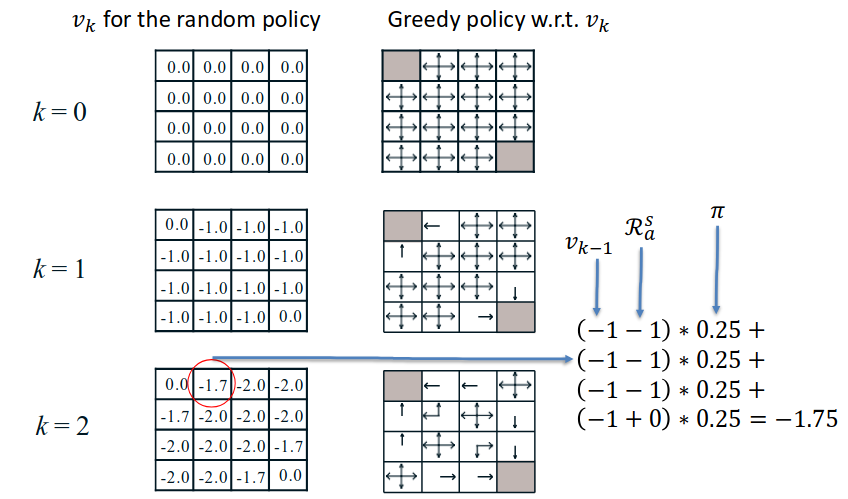
\includegraphics[width=0.9\textwidth]{images/L31.png}
    \caption{Example of prediction (left) and control (right). In the slides is showed that in the next time step the polict will remain the same, this means that the optimal polci has been reached. }
    \label{fig:student_markov_chain}
\end{figure}

\subsection{Policy Iteration}
\begin{wrapfigure}{r}{0.25\textwidth}
    \centering
    \vspace{-10pt}
    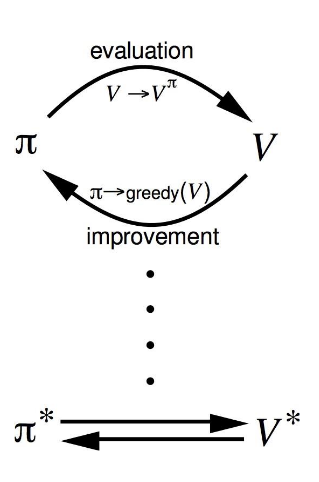
\includegraphics[width=\linewidth]{images/L32.png}
    \label{fig:TDlambda}
    \vspace{-10pt}
\end{wrapfigure}
La \emph{Policy Iteration} è il metodo di Dynamic Programming utilizzato per migliorare progressivamente una policy fino a ottenere una policy ottimale. L’idea di base consiste nell’alternare sistematicamente due fasi distinte: la valutazione della policy corrente e il suo miglioramento.

Il processo parte da una policy iniziale arbitraria $\pi$. Nella fase di \emph{policy evaluation}, la policy $\pi$ viene valutata calcolando la corrispondente value function $v^\pi$. Questa funzione rappresenta il return atteso partendo da ciascuno stato e seguendo sempre la policy $\pi$, ed è definita come:
\[
v^\pi(s) = \mathbb{E}_\pi \left[ R_{t+1} + \gamma R_{t+2} + \gamma^2 R_{t+3} + \dots \mid S_t = s \right]
\]
In pratica, $v^\pi$ viene stimata mediante l’Iterative Policy Evaluation, applicando ripetutamente la Bellman expectation equation fino alla convergenza.

Una volta ottenuta una stima accurata di $v^\pi$, si passa alla fase di \emph{policy improvement}. In questa fase, la policy viene aggiornata scegliendo, in ogni stato, l’azione che massimizza il valore atteso assumendo come riferimento la value function appena calcolata. La nuova policy $\pi'$ è definita come una policy greedy rispetto a $v^\pi$:
\[
\pi'(s) = \arg\max_{a \in \mathcal{A}} \sum_{s' \in \mathcal{S}} P_{ss'}^a \left[ R_s^a + \gamma v^\pi(s') \right]
\]
\begin{wrapfigure}{r}{0.3\textwidth}
    \centering
    \vspace{-10pt}
    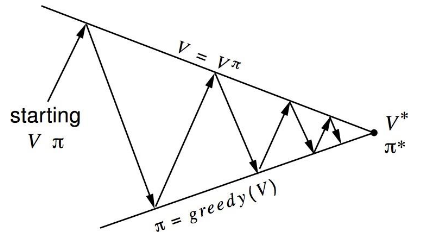
\includegraphics[width=\linewidth]{images/L33.png}
    \label{fig:TDlambda}
    \vspace{-10pt}
\end{wrapfigure}
Questo passo garantisce che la nuova policy $\pi'$ sia almeno altrettanto buona della policy precedente, cioè $\pi' \ge \pi$ per ogni stato.

In alcuni problemi semplici, come il classico Small Gridworld, una singola iterazione di policy improvement è sufficiente a ottenere direttamente la policy ottimale, ovvero si ha $\pi' = \pi^*$. In generale, tuttavia, è necessario ripetere più volte le due fasi di valutazione e miglioramento. Questo processo iterativo continua alternando policy evaluation e policy improvement fino a quando la policy non cambia più.

Un risultato fondamentale della Dynamic Programming è che la Policy Iteration, assumendo una conoscenza completa dell’MDP e uno spazio degli stati e delle azioni finito, converge sempre alla policy ottimale $\pi^*$. Questo rende la Policy Iteration uno degli algoritmi di riferimento per il problema di control nei Markov Decision Processes.

\subsection{Policy Improvement}

La \emph{Policy Improvement} è il passo che consente di migliorare una policy a partire dalla sua value function. Si consideri una policy deterministica $\pi$, tale che a ogni stato $s$ venga associata un’azione $a = \pi(s)$. Supponendo di conoscere la value function $v^\pi$, è possibile definire la corrispondente action-value function $q^\pi(s,a)$, che rappresenta il return atteso partendo dallo stato $s$, eseguendo l’azione $a$ e seguendo successivamente la policy $\pi$.

L’idea fondamentale del policy improvement consiste nel costruire una nuova policy $\pi'$ che, in ogni stato, selezioni in modo greedy l’azione che massimizza $q^\pi$. Formalmente, la policy migliorata è definita come:
\[
\pi'(s) = \arg\max_{a \in \mathcal{A}} q^\pi(s,a)
\]

Questa scelta garantisce un miglioramento locale del valore, poiché per ogni stato $s$ vale:
\[
q^\pi\bigl(s,\pi'(s)\bigr)
= \max_{a \in \mathcal{A}} q^\pi(s,a)
\ge q^\pi\bigl(s,\pi(s)\bigr)
= v^\pi(s)
\]

A partire da questa osservazione, è possibile dimostrare che la nuova policy $\pi'$ migliora la value function per tutti gli stati. In particolare:

\[
v^\pi(s)
\;\le\;
q^\pi\bigl(s,\pi'(s)\bigr)
\;=\;
\mathbb{E}_{\pi'} \left[ R_{t+1} + \gamma v^\pi(S_{t+1}) \mid S_t = s \right]
\;\le\;
\mathbb{E}_{\pi'} \left[ R_{t+1} + \gamma q^\pi\bigl(S_{t+1},\pi'(S_{t+1})\bigr) \mid S_t = s \right]
\]
\[
\le
\mathbb{E}_{\pi'} \left[ R_{t+1} + \gamma R_{t+2} + \gamma^2 q^\pi\bigl(S_{t+2},\pi'(S_{t+2})\bigr) \mid S_t = s \right]
\]
\[
\le\;
\mathbb{E}_{\pi'} \left[ R_{t+1} + \gamma R_{t+2} + \gamma^2 R_{t+3} + \dots \mid S_t = s \right]
=
v^{\pi'}(s)
\]

Da questa catena segue che:
\[
v^{\pi'}(s) \ge v^\pi(s) \qquad \forall s \in \mathcal{S}
\]
ovvero la policy $\pi'$ è almeno altrettanto buona della policy $\pi$ in tutti gli stati.

Se il processo di miglioramento non produce ulteriori cambiamenti, allora per ogni stato $s$ vale:
\[
q^\pi\bigl(s,\pi'(s)\bigr)
=
\max_{a \in \mathcal{A}} q^\pi(s,a)
=
q^\pi\bigl(s,\pi(s)\bigr)
=
v^\pi(s)
\]

In questo caso, la value function soddisfa l’equazione di Bellman di ottimalità:
\[
v^\pi(s) = \max_{a \in \mathcal{A}} q^\pi(s,a)
\]

Di conseguenza:
\[
v^\pi(s) = v^*(s) \qquad \forall s \in \mathcal{S}
\]
e quindi la policy $\pi$ è una policy ottimale.

\section{Modified Policy Iteration e Generalized Policy Iteration}

Nella Policy Iteration classica, ad ogni passo si eseguono due fasi distinte: si valuta la policy corrente $\pi$ fino a convergenza ottenendo $v^\pi$, e poi si migliora la policy rendendola greedy rispetto a $v^\pi$. In pratica, però, non è sempre necessario portare la policy evaluation fino alla convergenza esatta.

L’idea della \emph{Modified Policy Iteration} è proprio quella di \emph{interrompere prima} la policy evaluation. Invece di calcolare $v^\pi$ con accuratezza arbitraria, si può:
\begin{compactitemize}
    \item fermare l’Iterative Policy Evaluation quando la value function cambia meno di una certa soglia $\varepsilon$ (criterio di $\varepsilon$-convergenza),
    \item oppure semplicemente eseguire un numero fisso di iterazioni $k$ di policy evaluation e poi passare subito al policy improvement.
\end{compactitemize}

In altre parole, si alternano passi di valutazione \emph{parziale} della policy con passi di miglioramento greedy. Nel caso estremo in cui ci si fermi dopo una sola iterazione di policy evaluation ($k = 1$), la policy viene aggiornata ad ogni singola iterazione: questo caso limite risulta strettamente collegato alla \textbf{Value Iteration}.

Questa visione più generale del processo prende il nome di \textbf{Generalized Policy Iteration} (GPI). In GPI, qualunque algoritmo di policy evaluation (anche approssimato o tronco) può essere combinato con qualunque schema di policy improvement (ad esempio improvement greedy o $\varepsilon$-greedy). L’idea di fondo è che valutazione e miglioramento vengano portati avanti insieme, influenzandosi a vicenda, fino alla convergenza verso una policy ottimale.


\subsection{Principle of Optimality}

Il \emph{principle of optimality} formalizza una proprietà chiave delle policy ottimali nei Markov Decision Processes. Intuitivamente, afferma che una policy è ottimale se, oltre a essere ottimale a partire dallo stato iniziale, \emph{continua ad essere ottimale da ogni stato raggiungibile}.

Più precisamente, il teorema dice che una policy $\pi$ soddisfa
\[
v^\pi(s) = v^*(s)
\]
per uno stato $s$ se e solo se, per ogni stato $s'$ raggiungibile da $s$, la stessa policy è ottimale anche in $s'$, ossia
\[
v^\pi(s') = v^*(s') \quad \text{per tutti gli stati } s' \text{ raggiungibili da } s.
\]

Un modo equivalente di interpretarlo è: una policy ottimale può essere vista come composta da due parti: una \emph{prima azione ottimale} $A^*$ nello stato corrente, seguita da una policy che è a sua volta ottimale a partire dallo stato successore $S'$. Questo giustifica l’uso di equazioni ricorsive come la Bellman optimality equation: se conosciamo la soluzione dei “sottoproblemi” (gli stati successivi), possiamo ricostruire la soluzione dallo stato corrente.


\subsection{Deterministic Value Iteration}

La Deterministic Value Iteration è un metodo di Dynamic Programming utilizzato per calcolare direttamente la value function ottimale $v^*$ assumendo una conoscenza completa del modello dell’MDP. L’idea centrale è che, se fossero già noti i valori ottimali degli stati successivi $v^*(s')$, allora il valore ottimale di uno stato $s$ potrebbe essere calcolato immediatamente effettuando un one-step lookahead.

Questo principio è formalizzato dalla Bellman optimality equation, che nella Value Iteration viene utilizzata come regola di aggiornamento iterativo:
\[
v^*(s) \leftarrow \max_{a \in \mathcal{A}} \left( R_s^a + \gamma \sum_{s' \in \mathcal{S}} P_{ss'}^a \, v^*(s') \right)
\]

Questa equazione esprime il seguente meccanismo: per ogni stato $s$, si considerano tutte le azioni disponibili e, per ciascuna azione, si valuta il reward immediato atteso sommato al valore scontato degli stati successivi. Tra tutte le azioni, viene scelta quella che massimizza questo valore atteso. Il risultato rappresenta il miglior valore ottenibile partendo da $s$ e agendo in modo ottimale.

Poiché inizialmente i valori ottimali $v^*(s)$ non sono noti, la Value Iteration applica ripetutamente questo aggiornamento partendo da una stima iniziale arbitraria della value function. A ogni iterazione, i valori vengono raffinati utilizzando le stime precedenti, facendo dipendere il valore di uno stato dai valori degli stati successivi. In questo modo, l’informazione sui reward finali viene progressivamente propagata all’indietro nello spazio degli stati.

L’intuizione è quella di iniziare dagli stati terminali, o dagli stati con reward noti, e lavorare a ritroso verso tutti gli altri stati. Anche in presenza di cicli e di dinamiche stocastiche, il processo converge grazie all’uso del valore atteso sulle transizioni e al fattore di sconto $\gamma$, che garantisce la stabilità dell’aggiornamento. Una volta che la value function è conversa , la policy ottimale può essere ottenuta scegliendo, in ogni stato, l’azione greedy rispetto alla value function ottimale.


Nonostante il nome “deterministic value iteration” nei lucidi, l’algoritmo funziona perfettamente anche in MDP con transizioni stocastiche e con strutture con cicli (\emph{loopy MDP}), poiché le probabilità di transizione $P_{ss'}^a$ sono già incorporate nel calcolo dell’aspettativa. In sintesi, la Value Iteration aggiorna iterativamente i valori degli stati tramite la Bellman optimality equation finché la value function non si stabilizza; da questa, si estrae poi la policy ottimale come policy greedy rispetto a $v^*$.
\begin{figure}[H]
    \centering
    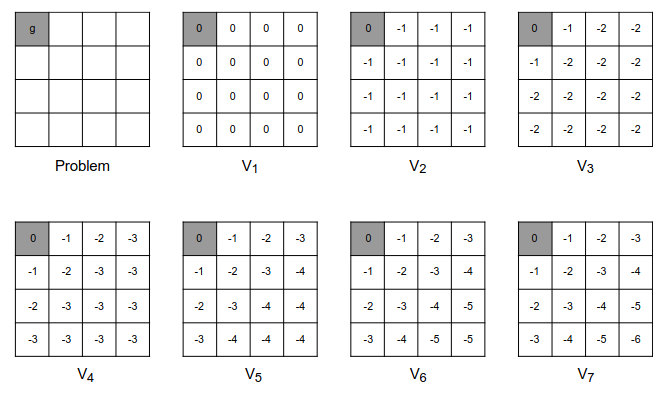
\includegraphics[width=0.9\textwidth]{images/L34.png}
    \caption{Example of backward value iteration }
    \label{fig:student_markov_chain}
\end{figure}

\subsection{Value Iteration: Control}

Il problema di control consiste nel determinare una policy ottimale $\pi^*$ partendo da una descrizione completa della dinamica dell’ambiente, ovvero dal modello dell’MDP. L’obiettivo è ottenere una policy che massimizzi il return atteso da ogni stato.

La Value Iteration risolve questo problema applicando iterativamente la Bellman optimality equation direttamente alla state-value function. A differenza della Policy Iteration, non viene mai mantenuta o valutata esplicitamente una policy durante il processo. L’algoritmo opera esclusivamente sui valori degli stati, aggiornandoli progressivamente fino alla convergenza verso la value function ottimale $v^*$.

L’aggiornamento fondamentale della Value Iteration è:
\[
v_{k+1}(s) = \max_{a \in \mathcal{A}} \left( R_s^a + \gamma \sum_{s' \in \mathcal{S}} P_{ss'}^a \, v_k(s') \right)
\]

A ogni iterazione $k+1$, per tutti gli stati $s \in \mathcal{S}$, il nuovo valore viene calcolato utilizzando esclusivamente i valori della precedente iterazione $v_k$. Questo aggiornamento è detto \emph{synchronous backup}, poiché tutti gli stati vengono aggiornati in parallelo a partire dalla stessa stima precedente.

La sequenza di value function $v_1 \rightarrow v_2 \rightarrow \dots$ converge progressivamente verso $v^*$, il fixed point della Bellman optimality equation. Durante questo processo non esiste una policy esplicita: le value function intermedie potrebbero non corrispondere ad alcuna policy reale. Solo una volta che la value function ha raggiunto la convergenza è possibile derivare una policy ottimale scegliendo, in ogni stato, l’azione greedy rispetto a $v^*$.

In sintesi, la Value Iteration può essere vista come la Bellman optimality equation trasformata in una regola di aggiornamento iterativa che consente di risolvere direttamente il problema di control.


\subsection{Synchronous Dynamic Programming Algorithms}

Gli algoritmi di Dynamic Programming sincroni condividono una struttura comune basata su aggiornamenti iterativi della value function. La distinzione principale tra i diversi algoritmi deriva dal tipo di equazione di Bellman utilizzata e dall’obiettivo del problema, che può essere di prediction o di control.

Nel caso della prediction, l’obiettivo è stimare la value function $v^\pi$ associata a una policy fissata. In questo scenario viene utilizzata la Bellman expectation equation e l’algoritmo risultante è l’Iterative Policy Evaluation.

Nel caso del control, l’obiettivo è calcolare la value function ottimale $v^*$. Questo può essere ottenuto in due modi diversi. Utilizzando la Bellman expectation equation insieme a un passo esplicito di policy improvement si ottiene la Policy Iteration, che alterna valutazione e miglioramento della policy. Utilizzando invece direttamente la Bellman optimality equation si ottiene la Value Iteration, che incorpora il miglioramento della policy nell’aggiornamento dei valori.

Tutti questi algoritmi operano tipicamente sulla state-value function. La complessità computazionale per ogni iterazione è dell’ordine di $O(mn^2)$, dove $n$ è il numero di stati e $m$ il numero di azioni. È possibile applicare concetti analoghi anche alla action-value function, ma in questo caso la complessità per iterazione cresce fino a $O(m^2 n^2)$, poiché è necessario considerare esplicitamente sia stati che coppie stato–azione.

Questa struttura sincrona, in cui tutti gli stati vengono aggiornati simultaneamente a ogni iterazione, rende gli algoritmi di Dynamic Programming concettualmente semplici e garantisce la convergenza, a patto di disporre di una conoscenza completa del modello dell’ambiente.
\begin{figure}[H]
    \centering
    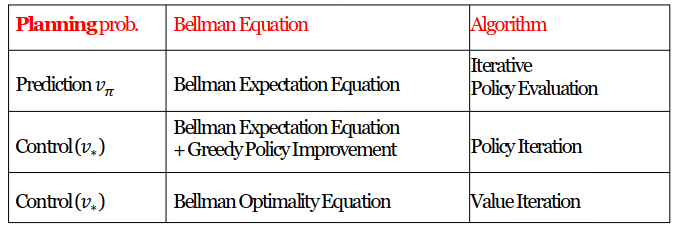
\includegraphics[width=0.9\textwidth]{images/F35.png}
    \label{fig:student_markov_chain}
\end{figure}

\section{Asynchronous Dynamic Programming}

Tutti i metodi di Dynamic Programming descritti finora utilizzano aggiornamenti sincroni (\emph{synchronous backups}), nei quali i valori di tutti gli stati vengono aggiornati in parallelo utilizzando la stessa stima precedente della value function. Questo approccio è concettualmente semplice, ma può risultare computazionalmente costoso quando il numero di stati è elevato.

L’Asynchronous Dynamic Programming introduce una strategia alternativa in cui gli stati vengono aggiornati individualmente, uno alla volta, e in un ordine arbitrario. A ogni passo, viene selezionato un singolo stato e su di esso viene applicato l’aggiornamento di Bellman appropriato, utilizzando immediatamente i valori più recenti disponibili. In questo modo, gli aggiornamenti non avvengono più in parallelo, ma in modo incrementale.

Questo approccio può ridurre significativamente il costo computazionale, poiché non è necessario aggiornare tutti gli stati a ogni iterazione. Inoltre, permette di concentrare il calcolo sugli stati più rilevanti o più frequentemente visitati. Nonostante la mancanza di sincronizzazione, è garantito che gli algoritmi asincroni convergano alla soluzione corretta, a patto che tutti gli stati continuino a essere selezionati e aggiornati nel tempo.

Esistono diversi criteri per scegliere quale stato aggiornare a ogni passo. Uno dei più semplici e fondamentali è il seguente.

\begin{compactitemize}
    \item \textbf{In-place Dynamic Programming}
    \item \textbf{Prioritized sweeping}
    \item \textbf{Real-Time dynamic programming}
\end{compactitemize}

\subsection{In-Place Dynamic Programming}

Nella Value Iteration sincrona classica, l’algoritmo mantiene due copie distinte della value function: una versione precedente $v_{\text{old}}$ e una versione aggiornata $v_{\text{new}}$. A ogni iterazione, per tutti gli stati $s \in \mathcal{S}$, il nuovo valore viene calcolato utilizzando esclusivamente $v_{\text{old}}$ secondo:
\[
v_{\text{new}}(s) \leftarrow \max_{a \in \mathcal{A}} \left( R_s^a + \gamma \sum_{s' \in \mathcal{S}} P_{ss'}^a \, v_{\text{old}}(s') \right)
\]
Al termine dell’aggiornamento di tutti gli stati, la copia vecchia viene sostituita con la nuova:
\[
v_{\text{old}}(s) \leftarrow v_{\text{new}}(s) \qquad \forall s \in \mathcal{S}
\]
Questo schema garantisce che tutti i backup utilizzino la stessa value function di riferimento, ma richiede di memorizzare due copie della value function e rallenta la propagazione dell’informazione, perché i nuovi valori non vengono sfruttati finché l’intera iterazione non è terminata.

Nell’In-Place Dynamic Programming, invece, si utilizza una sola copia della value function. Quando uno stato $s$ viene aggiornato, il suo valore viene immediatamente sovrascritto e reso disponibile per gli aggiornamenti successivi. L’aggiornamento assume la forma:
\[
v(s) \leftarrow \max_{a \in \mathcal{A}} \left( R_s^a + \gamma \sum_{s' \in \mathcal{S}} P_{ss'}^a \, v(s') \right)
\]
In questo modo, se uno stato successore $s'$ è già stato aggiornato nella stessa passata, il nuovo valore di $v(s')$ viene immediatamente utilizzato; se non lo è, viene utilizzato il valore precedente. Questo schema accelera la propagazione dell’informazione nello spazio degli stati ed è concettualmente analogo al metodo di Gauss--Seidel per la risoluzione di sistemi lineari. Pur introducendo una dipendenza dall’ordine di aggiornamento, l’In-Place Dynamic Programming garantisce comunque la convergenza alla value function corretta, a condizione che tutti gli stati vengano aggiornati ripetutamente.



\subsection{Prioritized Sweeping}

Il Prioritized Sweeping è una strategia di Asynchronous Dynamic Programming che affronta esplicitamente il problema di decidere quali stati aggiornare per primi e in quale ordine. L’idea di base è concentrare il calcolo sugli stati per i quali l’aggiornamento potrebbe produrre il maggiore cambiamento nella value function.

Per ogni stato $s$ viene calcolato il \emph{Bellman error}, definito come:
\[
\left| \max_{a \in \mathcal{A}} \left( R_s^a + \gamma \sum_{s' \in \mathcal{S}} P_{ss'}^a \, v(s') \right) - v(s) \right|
\]

Questo valore misura quanto l’attuale stima di $v(s)$ sia incoerente con la Bellman optimality equation. L’algoritmo seleziona quindi per l’aggiornamento lo stato con il Bellman error più grande, poiché è quello per cui l’update è potenzialmente più informativo.

Dopo aver aggiornato uno stato, anche gli stati che possono transire verso di esso (i cosiddetti predecessori) devono essere rivalutati, poiché il loro valore potrebbe dipendere dal nuovo valore appena calcolato. Questo richiede la conoscenza delle dinamiche inverse dell’ambiente. Dal punto di vista implementativo, il Prioritized Sweeping può essere realizzato in modo efficiente utilizzando una coda di priorità che ordina gli stati in base al loro Bellman error.


\subsection{Real-Time Dynamic Programming}

Il Real-Time Dynamic Programming (RTDP) combina i principi della Dynamic Programming con l’esperienza diretta di un agente che interagisce con l’ambiente. A differenza degli altri metodi, non viene considerato l’intero spazio degli stati, ma solo quelli effettivamente rilevanti per l’agente.

L’algoritmo prevede che un agente esegua episodi nell’ambiente seguendo una policy (tipicamente greedy rispetto alla value function corrente). Dopo ogni time-step, una volta osservati lo stato $S_t$, l’azione $A_t$ e il reward $R_{t+1}$, viene aggiornato esclusivamente il valore dello stato corrente $S_t$ secondo:
\[
v(S_t) \leftarrow \max_{a \in \mathcal{A}} \left( R_{S_t}^a + \gamma \sum_{s' \in \mathcal{S}} P_{S_t s'}^a \, v(s') \right)
\]

In questo modo, solo gli stati visitati dall’agente vengono aggiornati, evitando di sprecare calcolo su stati che non sono rilevanti per il comportamento reale. Il RTDP può essere visto come una forma di Dynamic Programming focalizzata online, che utilizza il modello dell’ambiente ma restringe gli aggiornamenti allo spazio di stati effettivamente esplorato. Se l’agente continua a visitare ripetutamente tutti gli stati rilevanti, il metodo converge alla value function ottimale.

\section{Full-Width Backups}

I metodi di Dynamic Programming utilizzano \emph{full-width backups}, ovvero aggiornamenti in cui, per ogni stato selezionato, vengono considerati esplicitamente tutte le azioni disponibili e tutti gli stati successori. Sia nel caso di backup sincroni sia asincroni, l’aggiornamento di un singolo stato richiede l’uso completo del modello dell’MDP, includendo le probabilità di transizione e la reward function.

Questo approccio consente di calcolare aggiornamenti esatti e garantisce la convergenza agli obiettivi di prediction o control. Per questo motivo, la Dynamic Programming risulta efficace per problemi di dimensione media, anche con milioni di stati, purché il modello dell’ambiente sia noto e gestibile.

Tuttavia, nei problemi di grandi dimensioni, la Dynamic Programming è pesantemente limitata dalla cosiddetta \emph{Bellman’s curse of dimensionality}. Il numero di stati $n = |\mathcal{S}|$ cresce esponenzialmente con il numero di variabili di stato, rendendo rapidamente proibitivo il costo computazionale. In tali scenari, anche un singolo full-width backup può risultare troppo costoso, rendendo necessarie tecniche alternative basate su approssimazione, campionamento o apprendimento diretto dall’esperienza.



\chapter{Model-Free prediction}

In questa lezione affrontiamo il problema della \textbf{model-free prediction}, ovvero
la stima della funzione valore di una policy \textbf{senza conoscere il modello dell’ambiente}.
In particolare, analizziamo i principali algoritmi di \textit{policy evaluation}:

\begin{compactitemize}
    \item \textbf{Monte Carlo}
    \item \textbf{TD(0)}
    \item \textbf{TD($\lambda$)}
\end{compactitemize}

Il contesto è il seguente: assumiamo di avere una policy fissata $\pi$ e vogliamo stimare
la sua \textbf{state-value function} $v^\pi(s)$ osservando esclusivamente episodi di esperienza
generati seguendo $\pi$.

\section{Monte-Carlo}

I metodi \textbf{Monte Carlo} stimano la funzione valore utilizzando il ritorno
\textit{completo} degli episodi.
Essi non richiedono alcuna conoscenza del modello dell’ambiente e aggiornano le stime
solo dopo che un episodio è terminato.

\noindent
L’obiettivo è:

\[
\text{Reinforcement goal: learn } v^\pi \text{ from episodes of experience under policy } \pi
\]

Osserviamo episodi di esperienza della forma:
\[
S_1, A_1, R_2, \dots, S_T \sim \pi
\]

Ricordiamo che il \textbf{return} a partire dal tempo $t$ è definito come:
\[
G_t = R_{t+1} + \gamma R_{t+2} + \dots + \gamma^{T-1-t} R_T
\]

Il return rappresenta la ricompensa totale scontata che l’agente ottiene a partire dallo
stato $S_t$ fino alla fine dell’episodio.

La \textbf{value function} di una policy $\pi$ è definita come il valore atteso del return:
\[
v^\pi(s) = \mathbb{E}_\pi \left[ G_t \mid S_t = s \right]
\]

Poiché l’aspettativa non è direttamente calcolabile, Monte Carlo policy evaluation
la approssima tramite la \textbf{media empirica dei return osservati}.

\subsection{First-Visit Monte-Carlo}

Nel \textbf{First-Visit Monte-Carlo}, per ciascuno stato $s$ consideriamo solo
la \textbf{prima volta} in cui esso viene visitato all’interno di un episodio.

Per valutare uno stato $s$:

\begin{compactitemize}
    \item identifichiamo il primo time-step $t$ dell’episodio tale che $S_t = s$;
    \item incrementiamo il numero di visite:
    \[
    N(s) \leftarrow N(s) + 1
    \]
    \item accumuliamo il return osservato:
    \[
    S(s) \leftarrow S(s) + G_t
    \]
\end{compactitemize}

La stima del valore è data dalla media:
\[
V(s) = \frac{S(s)}{N(s)}
\]

Grazie alla legge dei grandi numeri, questa stima converge al valore vero:
\[
V(s) \xrightarrow[N(s)\to\infty]{} v^\pi(s)
\]

\subsection{Every-Visit Monte-Carlo}

Nel \textbf{Every-Visit Monte-Carlo}, si utilizza invece \textbf{ogni visita} allo stato $s$
in un episodio, non solo la prima.

Per valutare uno stato $s$:

\begin{compactitemize}
    \item per ogni time-step $t$ tale che $S_t = s$;
    \item incrementiamo il contatore:
    \[
    N(s) \leftarrow N(s) + 1
    \]
    \item accumuliamo il return:
    \[
    S(s) \leftarrow S(s) + G_t
    \]
\end{compactitemize}

Anche in questo caso la stima è la media:
\[
V(s) = \frac{S(s)}{N(s)}
\]

e vale la convergenza:
\[
V(s) \xrightarrow[N(s)\to\infty]{} v^\pi(s)
\]

\noindent
La differenza principale rispetto al First-Visit è che qui alcune visite allo stesso stato
possono contribuire più volte all’apprendimento, riducendo talvolta la varianza
ma introducendo maggiore correlazione tra i campioni.

\subsection{Incremental Mean}

Per calcolare le medie in modo efficiente, senza memorizzare tutti i return osservati,
si utilizza una forma incrementale.

Data una sequenza $x_1, x_2, \dots$, la media:
\[
\mu_k = \frac{1}{k} \sum_{j=1}^{k} x_j
\]

può essere aggiornata come:
\[
\mu_k
=
\mu_{k-1}
+
\frac{1}{k}
\left(
x_k - \mu_{k-1}
\right)
\]

Questa relazione è alla base degli aggiornamenti incrementali Monte Carlo.

\subsection{Incremental Monte-Carlo Policy Evaluation}

Dopo aver osservato un intero episodio:
\[
S_1, A_1, R_2, \dots, S_T
\]

per ciascuno stato $S_t$ visitato con return $G_t$, si aggiornano:

\[
N(S_t) \leftarrow N(S_t) + 1
\]

\[
V(S_t)
\leftarrow
V(S_t)
+
\frac{1}{N(S_t)}
\left(
G_t - V(S_t)
\right)
\]

\noindent
Questo aggiornamento equivale al calcolo incrementale della media dei return
associati allo stato $S_t$.

\subsection{Running Mean in Non-Stationary Problems}

Nei problemi non stazionari, in cui le statistiche dell’ambiente possono cambiare nel tempo,
può essere utile dare più peso alle esperienze recenti.

In questo caso si utilizza uno step-size costante $\alpha$:
\[
V(S_t)
\leftarrow
V(S_t)
+
\alpha
\left(
G_t - V(S_t)
\right)
\]

\noindent
Questa formulazione non converge alla media esatta, ma consente
di adattarsi più rapidamente ai cambiamenti dell’ambiente.

\section{Temporal-Difference Learning}

I metodi di \textbf{Temporal-Difference (TD) Learning} rappresentano una famiglia di algoritmi
model-free che stimano la funzione valore \textit{incrementalmente}, combinando
idee di Monte Carlo e Dynamic Programming.

A differenza dei metodi Monte Carlo, che attendono la fine dell’episodio,
i metodi TD aggiornano le stime \textbf{prima di conoscere l’esito finale},
sfruttando il \textbf{bootstrapping}.

\subsection{From Monte Carlo to Temporal-Difference}

L’obiettivo rimane lo stesso:
\[
\text{learn } v^\pi \text{ from experience under policy } \pi
\]

Nel caso Monte Carlo incrementale, l’aggiornamento è:
\[
V(S_t) \leftarrow V(S_t) + \alpha \big( G_t - V(S_t) \big)
\]

dove il valore viene aggiornato verso il \textit{return reale} $G_t$.
Questo richiede necessariamente la fine dell’episodio.

L’idea chiave di TD è sostituire il return completo con una \textbf{stima del return}.

\subsection{TD(0)}

Il più semplice algoritmo TD è \textbf{TD(0)}.
Invece di usare il return completo, TD(0) utilizza il target:
\[
R_{t+1} + \gamma V(S_{t+1})
\]

L’aggiornamento diventa:
\[
V(S_t) \leftarrow V(S_t)
+
\alpha \Big(
R_{t+1} + \gamma V(S_{t+1}) - V(S_t)
\Big)
\]

Dove:
\begin{compactitemize}
    \item $R_{t+1} + \gamma V(S_{t+1})$ è il \textbf{TD target}
    \item $R_{t+1} + \gamma V(S_{t+1}) - V(S_t)$ è il \textbf{TD error}
\end{compactitemize}

TD può essere visto come un metodo che:
\begin{quote}
\emph{aggiorna una stima verso un’altra stima (potenzialmente migliore)}
\end{quote}

\subsection{Online Learning and Bootstrapping}

Le proprietà fondamentali di TD learning sono:

\begin{compactitemize}
    \item è \textbf{model-free}: non richiede conoscenza di transizioni o reward;
    \item apprende \textbf{online}, dopo ogni singolo step;
    \item apprende anche da \textbf{episodi incompleti};
    \item sfrutta il bootstrapping, usando stime correnti per aggiornare altre stime.
\end{compactitemize}

Questo rende TD particolarmente adatto agli ambienti \textit{continuing}
(non terminanti).

\subsection{Bias--Variance Trade-Off}

Il confronto tra Monte Carlo e TD si spiega naturalmente in termini
di \textbf{bias} e \textbf{varianza}.

Il return Monte Carlo:
\[
G_t = R_{t+1} + \gamma R_{t+2} + \dots + \gamma^{T-1} R_T
\]

è uno stimatore:
\begin{compactitemize}
    \item \textbf{unbiased} di $v^\pi(S_t)$;
    \item ma ad \textbf{alta varianza}, poiché dipende da molte transizioni casuali.
\end{compactitemize}

Il \emph{vero} TD target:
\[
R_{t+1} + \gamma v^\pi(S_{t+1})
\]

sarebbe anch’esso unbiased, ma non è disponibile.

Il TD target utilizzato in pratica:
\[
R_{t+1} + \gamma V(S_{t+1})
\]

è:
\begin{compactitemize}
    \item \textbf{biased} (dipende da una stima);
    \item ma con \textbf{varianza molto più bassa} rispetto a $G_t$.
\end{compactitemize}

\subsection{Advantages and Disadvantages of MC vs TD}

\paragraph{Monte Carlo}
\begin{compactitemize}
    \item zero bias, alta varianza;
    \item buone proprietà di convergenza;
    \item funziona bene anche con function approximation non lineare;
    \item poco sensibile ai valori iniziali;
    \item richiede episodi completi;
    \item applicabile solo a problemi episodici.
\end{compactitemize}

\paragraph{Temporal-Difference}
\begin{compactitemize}
    \item bias non nullo, varianza ridotta;
    \item apprendimento online e incrementale;
    \item può apprendere da sequenze incomplete;
    \item adatto a problemi continuing;
    \item più efficiente in ambienti Markoviani;
    \item più sensibile ai valori iniziali.
\end{compactitemize}

\subsection{Batch Monte Carlo vs Batch TD}

Supponiamo di avere un dataset finito di $K$ episodi:
\[
\{ s_1^k, a_1^k, r_2^k, \dots, s_{T_k}^k \}_{k=1}^K
\]

Ripetendo ciclicamente Monte Carlo o TD(0) sugli episodi:

\begin{compactitemize}
    \item Monte Carlo converge alla soluzione che minimizza il \textbf{mean squared error}
    rispetto ai return osservati:
    \[
    \sum_{k=1}^K \sum_{t=1}^{T_k}
    \big(
    G_t^k - V(s_t^k)
    \big)^2
    \]
    \item TD(0) converge alla soluzione del \textbf{maximum likelihood Markov model}
    che meglio spiega i dati:
    \[
    \hat{P}_{s,s'}^a
    =
    \frac{1}{N(s,a)}
    \sum_{k=1}^K
    \sum_{t=1}^{T_k}
    \mathbf{1}(s_t^k, a_t^k, s_{t+1}^k = s,a,s')
    \]

    \[
    \hat{R}_{s,s'}^{a}
    =
    \frac{1}{N(s,a)}
    \sum_{k=1}^{K}
    \sum_{t=1}^{T_k}
    \mathbf{1}
    \big(
    s_t^{k} = s,\;
    a_t^{k} = a,\;
    s_{t+1}^{k} = s'
    \big)
    \, r_t^{k}
    \]

\end{compactitemize}

\subsection{Certainty Equivalence}

TD learning sfrutta esplicitamente la \textbf{Markov property} dell’ambiente,
mentre Monte Carlo no.

Di conseguenza:
\begin{compactitemize}
    \item TD è generalmente più efficiente negli ambienti Markoviani;
    \item Monte Carlo può essere più efficace in ambienti non Markoviani.
\end{compactitemize}

\section{TD($\lambda$)}
\begin{wrapfigure}{r}{0.3\textwidth}
    \centering
    \vspace{-10pt}
    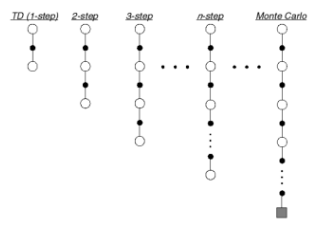
\includegraphics[width=\linewidth]{images/TDL.png}
    \label{fig:TDlambda}
    \vspace{-10pt}
\end{wrapfigure}

L'idea di TD($\lambda$) è quella di costruire un ponte continuo tra TD(0) e Monte Carlo,
combinando informazione a breve termine (pochi passi nel futuro)
e informazione a lungo termine (return completo).
Questo avviene introducendo prima gli \emph{$n$-step return}
e successivamente il \emph{$\lambda$-return}.

\subsection{$n$-step return}

Consideriamo una traiettoria generata sotto una policy $\pi$:
\[
S_1, A_1, R_2, S_2, A_2, R_3, \dots, S_T.
\]

Per lo stato $S_t$ possiamo definire diversi target, a seconda di quanto lontano
nel futuro vogliamo guardare.

Per $n = 1$ otteniamo il target TD(0):
\[
G_t^{(1)} = R_{t+1} + \gamma V(S_{t+1}).
\]

Per $n = 2$:
\[
G_t^{(2)} = R_{t+1} + \gamma R_{t+2} + \gamma^2 V(S_{t+2}).
\]

Per $n = \infty$ (episodio finito) otteniamo il return Monte Carlo:
\[
G_t^{(\infty)} =
R_{t+1} + \gamma R_{t+2} + \dots + \gamma^{T-t-1} R_T.
\]

In generale, l’\textbf{$n$-step return} è:
\[
G_t^{(n)} =
R_{t+1} + \gamma R_{t+2} + \dots + \gamma^{n-1} R_{t+n}
+ \gamma^n V(S_{t+n}),
\]
dove, se l’episodio termina prima, si smette semplicemente di bootstrappare.

L’aggiornamento \textbf{$n$-step TD} è:
\[
V(S_t) \leftarrow V(S_t) + \alpha \left(G_t^{(n)} - V(S_t)\right).
\]

Valori piccoli di $n$ producono target più biased ma a bassa varianza,
valori grandi di $n$ producono target meno biased ma più rumorosi.

\subsection{Media degli $n$-step return}

Invece di scegliere un singolo valore di $n$, possiamo combinare più $n$-step return.
Per esempio:
\[
\frac{1}{2} G_t^{(2)} + \frac{1}{2} G_t^{(4)}.
\]

L’idea generale è sfruttare informazione a diversi orizzonti temporali.
Il problema è farlo in modo teoricamente consistente ed efficiente.
La soluzione è il \textbf{$\lambda$-return}.

\subsection{Il $\lambda$-return}

Il $\lambda$-return combina \emph{tutti} gli $n$-step return con pesi geometrici:
\[
G_t^\lambda
=
(1 - \lambda)\sum_{n=1}^{\infty} \lambda^{n-1} G_t^{(n)},
\qquad 0 \le \lambda \le 1.
\]

I pesi $(1-\lambda)\lambda^{n-1}$ assegnano più importanza agli orizzonti temporali
vicini e riducono progressivamente il contributo di quelli più lontani.

Casi limite:
\begin{compactitemize}
    \item $\lambda = 0 \Rightarrow G_t^\lambda = G_t^{(1)}$ (TD(0));
    \item $\lambda \rightarrow 1 \Rightarrow$ comportamento Monte Carlo.
\end{compactitemize}

L’aggiornamento \textbf{forward-view TD($\lambda$)} è:
\[
V(S_t) \leftarrow V(S_t) + \alpha \left(G_t^\lambda - V(S_t)\right).
\]

\subsection{Forward e Backward View TD($\lambda$)}

La \textbf{forward view} descrive \emph{cosa} TD($\lambda$) sta stimando: la funzione valore viene
aggiornata verso il \textbf{$\lambda$-return} $G_t^\lambda$, che combina tutti gli $n$-step return.
Poiché $G_t^\lambda$ dipende dai reward futuri, questa formulazione richiede episodi completi ed è
quindi concettualmente simile ai metodi Monte Carlo.

La \textbf{backward view} descrive invece \emph{come} implementare TD($\lambda$) in pratica.
Attraverso le \textbf{eligibility traces}, l’errore TD calcolato a ogni passo viene propagato
agli stati visitati in passato, permettendo aggiornamenti \textbf{online} e incrementali, senza
attendere la fine dell’episodio.

In sintesi: la forward view fornisce il significato teorico di TD($\lambda$), mentre la backward view
fornisce il meccanismo computazionale efficiente che rende l’algoritmo utilizzabile in pratica.

\subsection{Eligibility Traces}

Le \textbf{eligibility traces} costituiscono il meccanismo fondamentale della backward view di
TD($\lambda$) e forniscono una soluzione al cosiddetto \emph{credit assignment problem}, ovvero il
problema di determinare quali stati passati siano responsabili di una ricompensa osservata nel
presente. In un processo decisionale sequenziale, una ricompensa tardiva può infatti dipendere da
azioni o stati visitati molto prima, rendendo non banale l’assegnazione del merito.

Due euristiche intuitive emergono naturalmente in questo contesto. La prima è la
\emph{frequency heuristic}, secondo cui gli stati visitati più frequentemente dovrebbero ricevere
maggiore credito. La seconda è la \emph{recency heuristic}, che privilegia invece gli stati visitati
più di recente. Le eligibility traces combinano entrambe le idee, assegnando a ogni stato una traccia
che cresce quando lo stato viene visitato e decade esponenzialmente nel tempo.

Formalmente, a ogni stato $s$ è associata una eligibility trace $E_t(s)$, inizializzata a zero.
Al tempo $t$, la trace viene aggiornata come
\[
E_t(s) = \gamma \lambda E_{t-1}(s) + \mathbb{1}(S_t = s),
\]
dove $\gamma$ è il fattore di sconto, $\lambda \in [0,1]$ controlla la velocità di decadimento della
traccia e $\mathbb{1}(S_t = s)$ vale 1 se lo stato corrente è $s$ e 0 altrimenti. In questo modo, uno
stato visitato di recente avrà una trace elevata, mentre il contributo degli stati più lontani nel
tempo diminuisce progressivamente.

Nella \textbf{backward-view TD($\lambda$)}, l’errore di differenza temporale
\[
\delta_t = R_{t+1} + \gamma V(S_{t+1}) - V(S_t)
\]
viene calcolato a ogni passo temporale e utilizzato per aggiornare il valore di tutti gli stati,
pesando l’aggiornamento con la rispettiva eligibility trace. L’aggiornamento della funzione valore è
dato da
\[
V(s) \leftarrow V(s) + \alpha \, \delta_t \, E_t(s),
\]
dove $\alpha$ è il passo di apprendimento. In questo modo, l’errore corrente viene propagato
all’indietro lungo la sequenza di stati visitati, in misura tanto maggiore quanto più lo stato è stato
frequente e recente.

La backward view può essere interpretata come se, a ogni passo, lo stato successivo $S_{t+1}$ fosse
trattato temporaneamente come uno stato terminale, producendo un aggiornamento immediato simile a TD
a un passo, ma distribuito retroattivamente grazie alle eligibility traces. Questo rende possibile
un apprendimento completamente \emph{online} e incrementale, pur mantenendo l’equivalenza teorica con
la forward view basata sui $\lambda$-return, almeno nel caso tabulare e con opportuni vincoli sui
parametri.

In sintesi, le eligibility traces permettono a TD($\lambda$) di coniugare le proprietà di bassa
varianza dei metodi TD con la capacità dei metodi Monte Carlo di assegnare il merito a intere
sequenze di stati, fornendo un compromesso controllato dal parametro $\lambda$.
\begin{figure}[H]
    \centering
    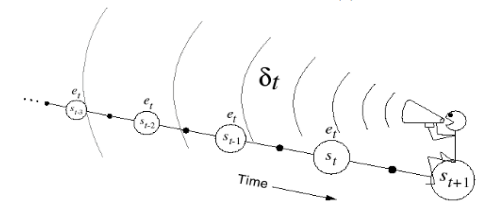
\includegraphics[width=0.6\textwidth]{images/TD2.png}
    \label{fig:student_markov_chain}
\end{figure}
\subsection{TD($\lambda$) e Monte Carlo}

Il parametro $\lambda$ in TD($\lambda$) regola il compromesso tra apprendimento basato su differenze
temporali e apprendimento Monte Carlo, controllando quanto lontano nel tempo venga assegnato il
credito. Al limite $\lambda = 0$, l’algoritmo coincide con TD a un passo, mentre per $\lambda = 1$ si
ottiene un comportamento equivalente ai metodi Monte Carlo nel caso di ambienti episodici e
aggiornamenti \emph{offline}. In quest’ultimo caso, l’aggiornamento effettivo del valore viene infatti
rinviato fino al termine dell’episodio.

L’equivalenza con Monte Carlo può essere compresa osservando l’errore di differenza temporale
$\delta_t = R_{t+1} + \gamma V(S_{t+1}) - V(S_t)$. Per $\lambda = 1$, la somma scontata degli errori TD
a partire da un istante $t$ presenta una proprietà di \emph{telescoping}:
\[
\delta_t + \gamma \delta_{t+1} + \gamma^2 \delta_{t+2} + \cdots + \gamma^{T-1-t} \delta_{T-1},
\]
che, una volta espansa, porta alla cancellazione progressiva dei termini di valore intermedi e si
riduce a
\[
G_t - V(S_t),
\]
dove $G_t$ è il return Monte Carlo. Questo mostra che l’errore totale accumulato da TD(1) su un
episodio coincide esattamente con quello utilizzato dai metodi Monte Carlo.

\subsection{Generalizzazione del telescoping in TD($\lambda$)}

La proprietà di telescoping si estende al caso generale $\lambda \in (0,1)$. In TD($\lambda$), gli
errori di differenza temporale vengono combinati secondo la sequenza
\[
\delta_t + \gamma \lambda \delta_{t+1} + (\gamma \lambda)^2 \delta_{t+2} + \cdots.
\]
Anche in questo caso, l’espansione mostra una cancellazione strutturata dei termini di valore, che
conduce al risultato
\[
G_t^\lambda - V(S_t),
\]
dove $G_t^\lambda$ è il $\lambda$-return della forward view. TD($\lambda$) può quindi essere visto
come un meccanismo che realizza il $\lambda$-return attraverso l’accumulo pesato degli errori TD.

\subsection{Forward e Backward View di TD($\lambda$)}

La relazione tra forward e backward view può essere chiarita considerando un episodio in cui uno
stato $s$ viene visitato una sola volta al tempo $k$. La eligibility trace associata evolve come
\[
E_t(s) =
\begin{cases}
0, & \text{se } t < k, \\
(\gamma \lambda)^{t-k}, & \text{se } t \ge k.
\end{cases}
\]
La backward view accumula gli aggiornamenti online tramite
\[
\sum_{t=1}^{T} \alpha \, \delta_t \, E_t(s)
=
\alpha \sum_{t=k}^{T} (\gamma \lambda)^{t-k} \delta_t,
\]
che, al termine dell’episodio, coincide con
\[
\alpha \bigl(G_k^\lambda - V(S_k)\bigr),
\]
ossia con l’aggiornamento della forward view basato sul $\lambda$-return. Nel caso di visite multiple
allo stesso stato, gli effetti delle diverse visite si sommano naturalmente attraverso le eligibility
traces.

\subsection{Equivalenza Offline e Online}

Nel regime di aggiornamenti \emph{offline}, in cui la funzione valore viene aggiornata solo al termine
dell’episodio, la forward view e la backward view di TD($\lambda$) sono perfettamente equivalenti e
producono identici aggiornamenti complessivi.

Nel regime \emph{online}, invece, gli aggiornamenti vengono applicati a ogni passo temporale. In
questo caso, la backward view costituisce un’approssimazione computazionalmente efficiente della
forward view, ma le due formulazioni non sono più esattamente identiche a causa della modifica
continua delle stime di valore durante l’episodio. Esistono tuttavia varianti, come l’\emph{exact
online TD($\lambda$)}, che ristabiliscono un’equivalenza completa anche nel caso online mediante una
definizione modificata delle eligibility traces.

\begin{figure}[H]
    \centering
    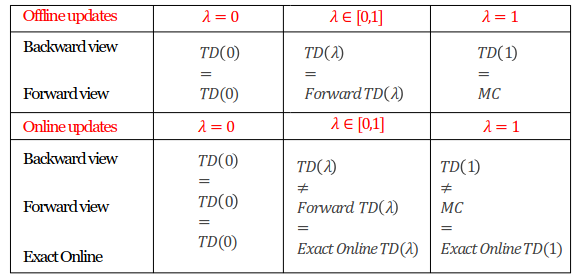
\includegraphics[width=0.9\textwidth]{images/TD3.png}
    \label{fig:student_markov_chain}
\end{figure}
\chapter{Model-Free Control}

La prima cosa che bisogna capire è la distinzione tra i seguenti due concetti:
\begin{compactitemize}
    \item \textbf{On-Policy Learning}: essenzialmente andiamo a utilizzare la stessa policy che andiamo ad aggiornare per muoverci all'intero dell'episodio: In termini tecnici si dice "Learn about policy $\pi$ from experience sampled from $\pi$.
    \item \textbf{Off-Policy Learning}: essenzialmente andiamo a utilizzare una policy (behavior) per muoverci all'interno degli episodi, e con quello che otteniamo andiamo ad aggioranre un'altra policy (target). In termini tecnici si dice "Learn about policy $\pi$ from experience sampled from $\mu$.
\end{compactitemize}

\subsection{Policy Iteration with Monte Carlo Evaluation}

Nel contesto del \textbf{model-free control}, l’obiettivo è determinare una policy ottimale senza assumere alcuna conoscenza esplicita del modello dell’MDP, ovvero senza conoscere né la funzione di transizione $P$ né la funzione di reward $R$. Questo vincolo ha conseguenze dirette sul modo in cui possono essere implementate le fasi di policy evaluation e policy improvement della policy iteration.

Si consideri innanzitutto il caso in cui si voglia applicare una classica relazione di policy iteration utilizzando la \textbf{state-value function} $v^\pi$. In un contesto model-based, il policy improvement si ottiene rendendo la policy greedy rispetto a $v^\pi$, cioè scegliendo, per ogni stato $s$, l’azione che massimizza l’espressione:
\[
R(s,a) + \gamma \sum_{s' \in \mathcal{S}} P(s' \mid s,a)\, v^\pi(s')
\]

Tuttavia, in un contesto model-free questa operazione non è realizzabile. Anche se fosse possibile stimare $v^\pi(s)$ tramite Monte Carlo, il passaggio di policy improvement richiede esplicitamente la conoscenza delle probabilità di transizione e dei reward attesi associati a ciascuna azione. In assenza del modello dell’MDP, non è possibile valutare l’effetto delle azioni sui futuri stati e, di conseguenza, non è possibile rendere la policy greedy rispetto alla state-value function.

Questo implica che una \textbf{policy iteration basata su $v^\pi$ non è compatibile con il paradigma model-free}. Il problema non risiede nella policy evaluation, che può essere effettuata tramite Monte Carlo usando l’esperienza episodica, bensì nel policy improvement, che richiede un one-step lookahead basato sul modello.

Per superare questa limitazione, il control model-free utilizza la \textbf{action-value function} $q^\pi(s,a)$. La funzione $q^\pi$ rappresenta il return atteso partendo dallo stato $s$, eseguendo l’azione $a$ e seguendo successivamente la policy $\pi$. A differenza di $v^\pi(s)$, essa associa direttamente un valore a ciascuna coppia stato–azione e incorpora implicitamente l’effetto della dinamica dell’ambiente.

Nel caso Monte Carlo, $q^\pi(s,a)$ può essere stimata come media dei ritorni osservati negli episodi ogni volta che la coppia $(s,a)$ viene visitata. Questo processo non richiede alcuna conoscenza del modello e si basa esclusivamente sull’esperienza campionata.

Una volta ottenuta una stima di $q^\pi$, il policy improvement diventa immediato: la policy viene aggiornata scegliendo, in ogni stato, l’azione che massimizza il valore dell’action-value function:
\[
\pi'(s) = \arg\max_{a \in \mathcal{A}} q^\pi(s,a)
\]
\begin{wrapfigure}{r}{0.4\textwidth}
    \centering
    \vspace{-10pt}
    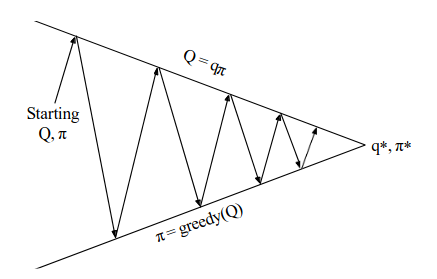
\includegraphics[width=\linewidth]{images/L51.png}
    \label{fig:TDlambda}
    \vspace{-10pt}
\end{wrapfigure}
Questo passo è completamente \textbf{model-free}, poiché non richiede né le probabilità di transizione né la funzione di reward. Tutta l’informazione necessaria per confrontare le azioni è contenuta nei valori stimati di $q^\pi$.

Il processo complessivo può quindi essere descritto come una \textbf{policy iteration model-free basata su action-value functions}, in cui:
\begin{compactitemize}
    \item la policy evaluation è realizzata tramite Monte Carlo estimation di $q^\pi$,
    \item la policy improvement è ottenuta rendendo la policy greedy rispetto a $q^\pi$.
\end{compactitemize}

Questo schema rientra nel quadro generale della \textbf{Generalized Policy Iteration}, in cui la stima di $q^\pi$ e l’aggiornamento della policy avvengono in modo iterativo fino alla convergenza verso l’action-value function ottimale $q^*$ e la policy ottimale $\pi^*$.

In sintesi, nel model-free control la scelta di lavorare con la action-value function non è solo conveniente, ma necessaria: mentre la state-value function non consente il policy improvement senza il modello dell’MDP, la action-value function permette di eseguire sia la valutazione sia il miglioramento della policy utilizzando esclusivamente l’esperienza osservata.
\begin{figure}[H]
    \centering
    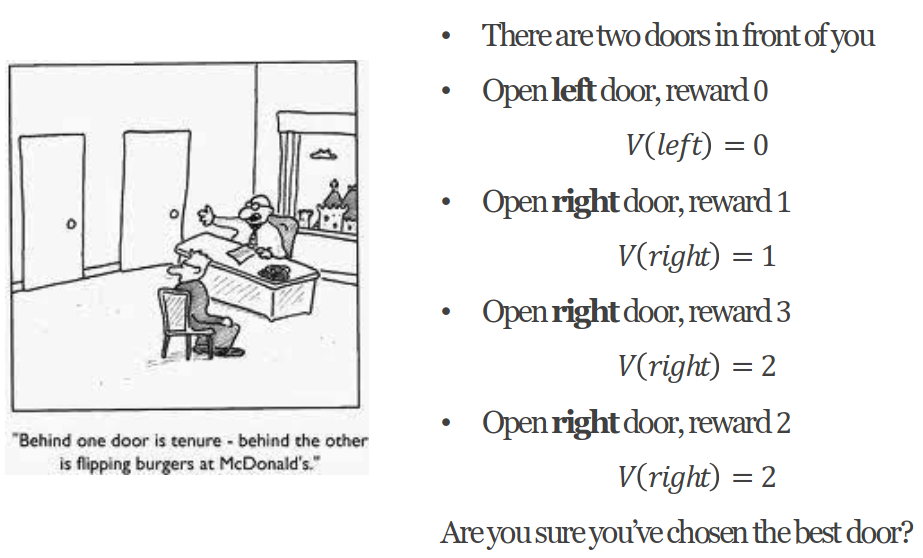
\includegraphics[width=0.7\textwidth]{images/L52.png}
    \caption{Esempio che mostra come, in presenza di reward stocastici o variabili nel tempo, una scelta apparentemente ottimale basata su poche osservazioni possa risultare subottimale. Sebbene una porta sembri inizialmente migliore, ulteriori esplorazioni possono rivelare valori medi diversi. L’esempio evidenzia quindi la necessità di bilanciare sfruttamento ed esplorazione, poiché basarsi solo sulla prima azione che massimizza il reward osservato non garantisce una decisione ottimale nel lungo periodo.}
    \label{fig:student_markov_chain}
\end{figure}

\section{$\epsilon$-Greedy Policies ed Exploration}

Nel control model-free, un problema centrale è garantire che l’agente continui a esplorare lo spazio delle azioni pur migliorando progressivamente la policy. Una policy puramente greedy, che seleziona sempre l’azione con valore stimato massimo, rischia infatti di convergere prematuramente verso una soluzione subottimale a causa di stime iniziali imprecise dei valori.

Una delle strategie più semplici ed efficaci per affrontare questo problema è l’uso delle \textbf{$\epsilon$-greedy policies}. L’idea fondamentale consiste nel bilanciare lo sfruttamento delle informazioni attualmente disponibili con una esplorazione casuale controllata.

Sia $Q(s,a)$ una stima dell’action-value function e sia $m = |\mathcal{A}|$ il numero di azioni disponibili. Una policy $\epsilon$-greedy rispetto a $Q$ è definita come:
\[
\pi(a \mid s) =
\begin{cases}
1 - \epsilon + \dfrac{\epsilon}{m} & \text{se } a \in \arg\max_{a' \in \mathcal{A}} Q(s,a') \\
\dfrac{\epsilon}{m} & \text{altrimenti}
\end{cases}
\]

Con probabilità $1 - \epsilon$ la policy seleziona un’azione greedy, ossia un’azione che massimizza il valore stimato $Q(s,a)$ nello stato $s$. Con probabilità $\epsilon$, invece, viene selezionata un’azione a caso, distribuita uniformemente tra tutte le azioni disponibili, incluse anche quelle greedy. In questo modo, tutte le azioni hanno sempre una probabilità strettamente positiva di essere esplorate.

Questa proprietà è cruciale nel model-free learning: garantire che ogni coppia stato–azione venga visitata sufficientemente spesso permette di migliorare progressivamente le stime di $Q(s,a)$ e ridurre l’effetto degli errori iniziali.


\subsection{$\epsilon$-Greedy Policy Improvement}

Le policy $\epsilon$-greedy non rappresentano soltanto una strategia di esplorazione, ma possono essere utilizzate anche come meccanismo di policy improvement all’interno della Generalized Policy Iteration.

Sia $\pi$ una policy $\epsilon$-greedy e sia $q^\pi$ la sua action-value function. Si consideri una nuova policy $\pi'$, definita come $\epsilon$-greedy rispetto a $q^\pi$. Per ogni stato $s$, il valore atteso di effettuare un’azione secondo $\pi'$ può essere scritto come:
\[
q^\pi\bigl(s, \pi'(s)\bigr)
= \sum_{a \in \mathcal{A}} \pi'(a \mid s)\, q^\pi(s,a)
\]

Sostituendo la definizione di policy $\epsilon$-greedy si ottiene:
\[
q^\pi\bigl(s, \pi'(s)\bigr)
=
\frac{\epsilon}{m} \sum_{a \in \mathcal{A}} q^\pi(s,a)
+
(1 - \epsilon) \max_{a \in \mathcal{A}} q^\pi(s,a)
\]

Poiché il valore massimo di $q^\pi(s,a)$ è sempre maggiore o uguale a qualunque combinazione convessa dei valori, segue che:
\[
\frac{\epsilon}{m} \sum_{a \in \mathcal{A}} q^\pi(s,a)
+
(1 - \epsilon) \max_{a \in \mathcal{A}} q^\pi(s,a)
\;\ge\;
\sum_{a \in \mathcal{A}} \pi(a \mid s)\, q^\pi(s,a)
=
v^\pi(s)
\]

Da questa disuguaglianza segue il seguente risultato fondamentale.

\medskip

\textbf{Teorema ($\epsilon$-Greedy Policy Improvement).}  
Per ogni policy $\epsilon$-greedy $\pi$, la policy $\pi'$ che è $\epsilon$-greedy rispetto a $q^\pi$ soddisfa:
\[
v^{\pi'}(s) \ge v^\pi(s) \qquad \forall s \in \mathcal{S}
\]

\medskip

Questo risultato mostra che il policy improvement non richiede necessariamente una policy puramente greedy. Anche introducendo esplorazione, è comunque garantito un miglioramento (o almeno un mantenimento) delle prestazioni in tutti gli stati.


\subsection{Monte Carlo Policy Iteration}
\begin{wrapfigure}{r}{0.4\textwidth}
    \centering
    \vspace{-10pt}
    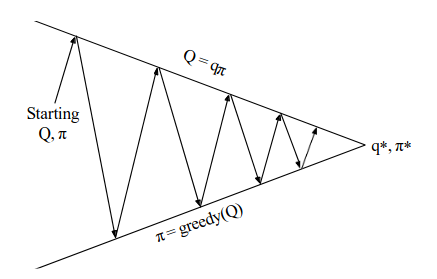
\includegraphics[width=\linewidth]{images/L51.png}
    \label{fig:TDlambda}
    \vspace{-10pt}
\end{wrapfigure}
Nel contesto del control model-free, la policy iteration può essere realizzata combinando:
\begin{compactitemize}
    \item una \textbf{policy evaluation} ottenuta tramite Monte Carlo estimation dell’action-value function,
    \item una \textbf{policy improvement} basata su una policy $\epsilon$-greedy.
\end{compactitemize}

Il processo parte da una stima iniziale di $Q$ e da una policy iniziale $\pi$. A ogni iterazione, vengono generati episodi completi seguendo la policy corrente $\pi$. Per ciascuna coppia stato–azione visitata, il valore $Q(s,a)$ viene aggiornato stimando il return medio osservato, ottenendo una nuova approssimazione di $q^\pi$.

Successivamente, la policy viene aggiornata rendendola $\epsilon$-greedy rispetto alla nuova stima di $Q$. Il procedimento può essere riassunto schematicamente come:
\[
Q \;\longrightarrow\; \pi = \epsilon\text{-greedy}(Q)
\;\longrightarrow\; Q \approx q^\pi
\;\longrightarrow\; \pi'
\]

Questo schema rappresenta una forma concreta di \textbf{Generalized Policy Iteration}, in cui policy evaluation e policy improvement avvengono in modo iterativo, approssimato e interdipendente. Al crescere del numero di episodi, e sotto opportune condizioni di esplorazione, il processo converge verso l’action-value function ottimale $q^*$ e una policy ottimale $\pi^*$.

\subsection{Monte Carlo Control}
\begin{wrapfigure}{r}{0.3\textwidth}
    \centering
    \vspace{-10pt}
    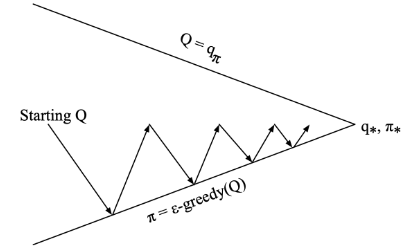
\includegraphics[width=\linewidth]{images/L53.png}
    \label{fig:TDlambda}
    \vspace{-10pt}
\end{wrapfigure}
Nel Monte Carlo Control, la policy evaluation e la policy improvement vengono eseguite dopo ogni episodio. Ogni episodio contribuisce a migliorare la stima di $Q$ e, di conseguenza, a rendere la policy sempre più orientata verso le azioni migliori, pur mantenendo una componente di esplorazione controllata tramite il parametro $\epsilon$.

In sintesi, l’uso di policy $\epsilon$-greedy consente di risolvere il problema del control in ambienti model-free garantendo contemporaneamente:
\begin{compactitemize}
    \item esplorazione continua di tutte le azioni,
    \item miglioramento monotono della policy,
    \item convergenza verso una policy ottimale.
\end{compactitemize}

\section{GLIE}

\subsection{Greedy in the Limit with Infinite Exploration}

Nel control model-free esiste una tensione fondamentale tra \textbf{esplorazione} e \textbf{sfruttamento}. Da un lato, per apprendere correttamente i valori delle azioni è necessario continuare a esplorare; dall’altro, per ottenere una policy ottimale nel lungo periodo è necessario agire in modo sempre più greedy rispetto alle stime dei valori.

Il concetto di \textbf{Greedy in the Limit with Infinite Exploration (GLIE)} formalizza una condizione che permette di risolvere questa tensione. Una sequenza di policy $\{\pi_k\}$ soddisfa la condizione GLIE se valgono entrambe le seguenti proprietà.

La prima proprietà è la \textbf{esplorazione infinita}. Ogni coppia stato–azione deve essere visitata un numero infinito di volte:
\[
\lim_{k \to \infty} N_k(s,a) = \infty \qquad \forall (s,a) \in \mathcal{S} \times \mathcal{A}
\]
Questa condizione garantisce che le stime dei valori non rimangano ancorate a osservazioni iniziali errate e che tutte le azioni abbiano la possibilità di essere valutate correttamente.

La seconda proprietà è la \textbf{convergenza greedily}. Nel limite, la policy deve diventare puramente greedy rispetto all’action-value function stimata:
\[
\lim_{k \to \infty} \pi_k(a \mid s)
=
\mathbf{1}\!\left(
a = \arg\max_{a' \in \mathcal{A}} Q_k(s,a')
\right)
\]
Nel lungo periodo, quindi, l’esplorazione viene progressivamente eliminata e la policy converge a una policy deterministica greedy.

Un esempio classico di policy GLIE è la policy $\epsilon$-greedy con un parametro di esplorazione decrescente nel tempo, ad esempio:
\[
\epsilon_k = \frac{1}{k}
\]
In questo caso, l’esplorazione è garantita per un tempo arbitrariamente lungo, ma tende a zero quando il numero di episodi cresce, assicurando una policy greedy nel limite.


\subsection{GLIE Monte-Carlo Control}

Il \textbf{GLIE Monte-Carlo Control} applica il principio GLIE all’algoritmo di Monte Carlo Control. L’idea è combinare:
\begin{compactitemize}
    \item una stima Monte Carlo dell’action-value function $q^\pi$,
    \item una policy $\epsilon$-greedy con $\epsilon$ decrescente nel tempo.
\end{compactitemize}

Il procedimento opera episodio per episodio. Al $k$-esimo episodio, viene generata una sequenza completa di stati, azioni e reward seguendo la policy corrente $\pi_k$:
\[
S_1, A_1, R_2, \dots, S_T \sim \pi_k
\]

Per ogni coppia $(S_t, A_t)$ visitata nell’episodio, viene incrementato il numero di visite:
\[
N(S_t, A_t) \leftarrow N(S_t, A_t) + 1
\]
e la stima dell’action-value function viene aggiornata tramite una media incrementale del return osservato:
\[
Q(S_t, A_t)
\leftarrow
Q(S_t, A_t)
+
\frac{1}{N(S_t, A_t)}
\Bigl(
G_t - Q(S_t, A_t)
\Bigr)
\]

Una volta aggiornati i valori $Q$, la policy viene migliorata rendendola $\epsilon_k$-greedy rispetto alla nuova stima:
\[
\pi_{k+1} = \epsilon_k\text{-greedy}(Q)
\]
con $\epsilon_k \to 0$ quando $k \to \infty$.

Questo schema soddisfa entrambe le condizioni GLIE: tutte le coppie stato–azione vengono esplorate infinitamente spesso e la policy diventa greedily ottimale nel limite. Di conseguenza, vale il seguente risultato fondamentale.

\medskip

\textbf{Teorema (Convergenza del GLIE Monte-Carlo Control).}  
Assumendo che l’MDP sia finito e che la sequenza di policy sia GLIE, l’algoritmo di GLIE Monte-Carlo Control converge con probabilità $1$ all’action-value function ottimale:
\[
Q(s,a) \longrightarrow q^*(s,a)
\qquad \forall (s,a) \in \mathcal{S} \times \mathcal{A}
\]
e la policy $\epsilon$-greedy converge a una policy ottimale $\pi^*$.

Questo risultato fornisce una garanzia teorica forte sulla correttezza del Monte Carlo Control, a patto di accettare l’ipotesi di episodi completi e una esplorazione sufficientemente lunga.


\subsection{Monte Carlo Control vs Temporal-Difference Control}

Sebbene il GLIE Monte-Carlo Control goda di solide garanzie teoriche, presenta alcune limitazioni pratiche. In particolare, l’aggiornamento dei valori avviene solo al termine di un episodio completo, una volta che il return totale $G_t$ è stato osservato. Questo rende il metodo intrinsecamente \textbf{offline} e comporta un’elevata varianza nelle stime.

Il \textbf{Temporal-Difference (TD) Control} nasce dall’idea di sostituire la stima Monte Carlo del return con una stima incrementale basata su informazioni parziali osservabili a ogni time-step. Invece di attendere la fine dell’episodio, il TD Control aggiorna direttamente l’action-value function dopo ogni transizione.

Dal punto di vista concettuale, il control TD mantiene la stessa struttura generale:
\begin{compactitemize}
    \item apprendimento diretto di $Q(s,a)$,
    \item policy improvement tramite policy $\epsilon$-greedy.
\end{compactitemize}

La differenza risiede nel metodo di valutazione. Mentre il Monte Carlo utilizza il return completo $G_t$, il TD Control utilizza una stima bootstrap che combina reward immediati e stime correnti dei valori futuri. Questo comporta diversi vantaggi: una varianza più bassa, la possibilità di apprendere online e la capacità di operare anche in presenza di sequenze incomplete o continue.

In questo senso, il TD Control può essere visto come un’evoluzione naturale del Monte Carlo Control, in cui la fase di policy evaluation viene resa più efficiente sostituendo il Monte Carlo con aggiornamenti temporally local. Questa idea costituisce la base di algoritmi fondamentali come SARSA e Q-learning, che rappresentano il fulcro del Reinforcement Learning model-free moderno.

\section{Sarsa Algorithm for On-Policy Control}

Il metodo \textbf{SARSA} è un algoritmo di control model-free e on-policy che apprende direttamente l’action-value function associata alla policy corrente. Il nome SARSA deriva dalla sequenza di variabili coinvolte nell’aggiornamento: stato $S_t$, azione $A_t$, reward $R_{t+1}$, stato successivo $S_{t+1}$ e azione successiva $A_{t+1}$.

Il controllo viene ottenuto applicando una \textbf{Generalized Policy Iteration} in cui policy evaluation e policy improvement avvengono a ogni time-step. L’algoritmo mantiene una stima $Q(s,a)$ dell’action-value function $q^\pi(s,a)$ e una policy $\pi$ tipicamente scelta come $\epsilon$-greedy rispetto a $Q$.

Ad ogni passo temporale, osservata la transizione $(S_t, A_t, R_{t+1}, S_{t+1}, A_{t+1})$, la stima di $Q$ viene aggiornata secondo la regola:
\[
Q(S_t, A_t) \leftarrow Q(S_t, A_t) + \alpha_t \, \delta_t
\]
dove il \textbf{TD-error} è definito come:
\[
\delta_t = R_{t+1} + \gamma Q(S_{t+1}, A_{t+1}) - Q(S_t, A_t)
\]

Questo aggiornamento è un esempio di \textbf{Temporal-Difference learning}, in cui il valore corrente viene corretto utilizzando una stima bootstrap del valore futuro invece di attendere il return completo. Poiché l’azione $A_{t+1}$ è selezionata dalla stessa policy che viene valutata, SARSA è un algoritmo intrinsecamente on-policy.

\begin{figure}[H]
    \centering
    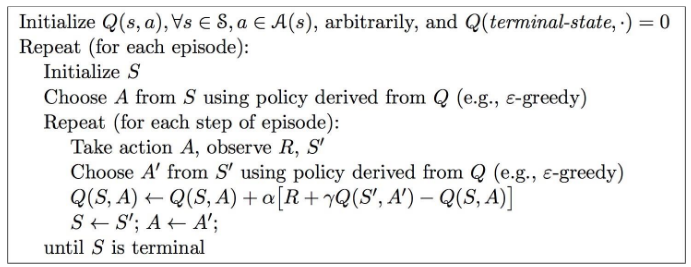
\includegraphics[width=0.9\textwidth]{images/L54.png}
    \caption{Algortimo Sarsa}
    \label{fig:student_markov_chain}
\end{figure}
\subsection{Convergence of Sarsa}

Sotto opportune condizioni, SARSA converge all’action-value function ottimale $q^*$ e la policy associata converge a una policy ottimale.

In particolare, la convergenza è garantita se la sequenza di policy $\{\pi_t\}$ soddisfa la condizione di \textbf{GLIE} e se i learning rates $\{\alpha_t\}$ soddisfano le condizioni di Robbins–Monro:
\[
\sum_{t=1}^{\infty} \alpha_t = \infty,
\qquad
\sum_{t=1}^{\infty} \alpha_t^2 < \infty
\]

La prima condizione assicura che ogni coppia stato–azione venga esplorata infinite volte, mentre la seconda garantisce che l’ampiezza degli aggiornamenti decresca sufficientemente nel tempo da stabilizzare le stime. Sotto queste ipotesi, la stima $Q(s,a)$ converge con probabilità $1$ alla funzione ottimale $q^*(s,a)$ e la policy $\epsilon$-greedy converge a una policy ottimale nel limite.


\subsection{n-Step Sarsa}

La versione standard di SARSA utilizza un aggiornamento a un singolo passo temporale (one-step), in cui il return è approssimato usando un solo reward futuro e la stima del valore al passo successivo. Questa idea può essere generalizzata introducendo i \textbf{n-step returns}, che combinano informazioni provenienti da più passi futuri.

Per $n = 1$, il one-step SARSA utilizza il return:
\[
q_t^{(1)} = R_{t+1} + \gamma Q(S_{t+1}, A_{t+1})
\]

Per $n = 2$, si ottiene:
\[
q_t^{(2)} = R_{t+1} + \gamma R_{t+2} + \gamma^2 Q(S_{t+2}, A_{t+2})
\]

Nel caso limite $n = \infty$, il return coincide con il return Monte Carlo:
\[
q_t^{(\infty)} = R_{t+1} + \gamma R_{t+2} + \gamma^2 R_{t+3} + \dots + \gamma^{T-1} R_T
\]

In generale, l’n-step Q-return è definito come:
\[
q_t^{(n)} =
R_{t+1}
+ \gamma R_{t+2}
+ \dots
+ \gamma^{n-1} R_{t+n}
+ \gamma^n Q(S_{t+n}, A_{t+n})
\]

L’aggiornamento di n-step SARSA diventa quindi:
\[
Q(S_t, A_t) \leftarrow Q(S_t, A_t)
+ \alpha \bigl( q_t^{(n)} - Q(S_t, A_t) \bigr)
\]

Variando il parametro $n$ è possibile ottenere un compromesso tra bias e varianza: valori piccoli di $n$ inducono maggiore bias ma minore varianza, mentre valori grandi di $n$ si avvicinano al comportamento Monte Carlo.


\subsection{Forward View Sarsa($\lambda$)}

L’algoritmo Sarsa($\lambda$) fornisce un meccanismo per combinare in modo continuo tutti gli n-step returns, senza dover scegliere esplicitamente un valore di $n$.

Nel \textbf{forward view}, si definisce il $\lambda$-return come una combinazione convessa di tutti gli n-step returns, pesata geometricamente:
\[
q_t^{\lambda}
=
(1 - \lambda)
\sum_{n=1}^{\infty}
\lambda^{n-1}
q_t^{(n)}
\]

Il parametro $\lambda \in [0,1]$ controlla l’importanza dei contributi a lungo termine. Per $\lambda = 0$ si ottiene il one-step SARSA, mentre per $\lambda \to 1$ il return tende al return Monte Carlo.

L’aggiornamento forward-view di Sarsa($\lambda$) è quindi:
\[
Q(S_t, A_t)
\leftarrow
Q(S_t, A_t)
+ \alpha \bigl( q_t^{\lambda} - Q(S_t, A_t) \bigr)
\]

Questa formulazione è principalmente di interesse teorico, poiché richiederebbe la conoscenza di ritorni futuri non ancora osservati.


\subsection{Backward View Sarsa($\lambda$)}

Per ottenere un algoritmo implementabile online, il forward view viene reso equivalente attraverso il \textbf{backward view}, che utilizza il concetto di \textbf{eligibility traces}. In questo approccio, viene mantenuta una traccia di eleggibilità per ogni coppia stato–azione.

Le eligibility traces sono inizializzate a zero:
\[
E_0(s,a) = 0 \qquad \forall (s,a)
\]

Ad ogni time-step, le tracce vengono aggiornate secondo:
\[
E_t(s,a) = \gamma \lambda E_{t-1}(s,a)
+ \mathbf{1}(S_t = s, A_t = a)
\]

In questo modo, le coppie stato–azione visitate recentemente mantengono un’eleggibilità elevata, che decade esponenzialmente nel tempo.

Il TD-error viene calcolato come nel SARSA standard:
\[
\delta_t = R_{t+1} + \gamma Q(S_{t+1}, A_{t+1}) - Q(S_t, A_t)
\]

Infine, l’action-value function viene aggiornata per tutte le coppie $(s,a)$ in proporzione al TD-error e alla rispettiva eligibility trace:
\[
Q(s,a) \leftarrow Q(s,a) + \alpha \, \delta_t \, E_t(s,a)
\]

Il backward view Sarsa($\lambda$) è computazionalmente efficiente, completamente online e, sotto opportune condizioni, equivalente al forward view in termini di comportamento asintotico.
\begin{figure}[H]
    \centering
    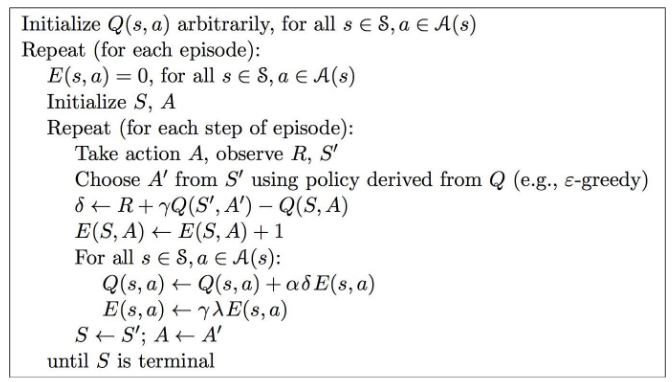
\includegraphics[width=0.9\textwidth]{images/L55.png}
    \caption{Algortimo Sarsa($\lambda$)}
    \label{fig:student_markov_chain}
\end{figure}

\section{Off-Policy Learning}

Nel Reinforcement Learning, il termine \emph{off-policy learning} indica la possibilità di valutare o migliorare una policy \emph{target} $\pi$ utilizzando esperienza generata da una policy diversa, detta \emph{behaviour policy} $\mu$. In questo contesto, l’obiettivo è stimare quantità come $v^\pi(s)$ o $q^\pi(s,a)$ mentre l’agente segue effettivamente la policy $\mu$.

Questa impostazione è particolarmente importante in diversi scenari pratici. Consente di apprendere osservando il comportamento di altri agenti o di esseri umani, di riutilizzare dati raccolti in passato con policy diverse e di apprendere una policy ottimale continuando a seguire una policy fortemente esplorativa. Inoltre, permette di valutare più policy differenti a partire da un’unica sorgente di esperienza.

Il problema centrale dell’off-policy learning è che le distribuzioni di probabilità indotte da $\pi$ e $\mu$ sugli episodi e sulle transizioni non coincidono. Per correggere questo disallineamento e ottenere stime corrette, è necessario introdurre il concetto di \textbf{importance sampling}.


\subsection{Importance Sampling}

L’importance sampling è una tecnica statistica che consente di stimare il valore atteso di una funzione rispetto a una distribuzione di probabilità utilizzando campioni generati da una distribuzione diversa.

Sia $X$ una variabile aleatoria e sia $f(X)$ una funzione integrabile. Il valore atteso di $f$ rispetto a una distribuzione $P$ è:
\[
\mathbb{E}_{X \sim P}[f(X)] = \sum_x P(x) f(x)
\]

Introducendo una seconda distribuzione $Q$, tale che $Q(x) > 0$ ogni volta che $P(x) > 0$, è possibile riscrivere l’aspettativa come:
\[
\mathbb{E}_{X \sim P}[f(X)]
=
\sum_x Q(x) \frac{P(x)}{Q(x)} f(x)
=
\mathbb{E}_{X \sim Q}
\left[
\frac{P(X)}{Q(X)} f(X)
\right]
\]

Il rapporto $\frac{P(X)}{Q(X)}$ è detto \textbf{importance sampling ratio} e misura quanto il campione estratto da $Q$ sia rappresentativo della distribuzione $P$. Applicando questa idea al Reinforcement Learning, l’importance sampling permette di correggere l’esperienza generata dalla behaviour policy $\mu$ affinché possa essere utilizzata per stimare quantità associate alla target policy $\pi$.

Una condizione fondamentale è che $\mu(a \mid s) > 0$ ogni volta che $\pi(a \mid s) > 0$; in caso contrario, il rapporto di importance sampling non è definito e l’apprendimento off-policy diventa impossibile.


\subsection{Importance Sampling for Off-Policy Monte-Carlo}

Nel contesto Monte-Carlo, l’obiettivo è stimare il return atteso sotto la policy target $\pi$ utilizzando episodi generati seguendo la behaviour policy $\mu$.

Poiché un episodio completo è una sequenza di azioni, è necessario correggere l’intero return utilizzando un prodotto di rapporti di importance sampling. Per un episodio che parte dal tempo $t$ e termina al tempo $T$, il coefficiente di correzione è definito come:
\[
\rho_{t:T}
=
\prod_{k=t}^{T}
\frac{\pi(A_k \mid S_k)}{\mu(A_k \mid S_k)}
\]

Il return corretto diventa quindi:
\[
G_t^{\pi/\mu} = \rho_{t:T} \, G_t
\]

La stima del valore viene aggiornata muovendosi verso questo return corretto:
\[
V(S_t)
\leftarrow
V(S_t) + \alpha
\bigl(
G_t^{\pi/\mu} - V(S_t)
\bigr)
\]

Questo aggiornamento è una stima non distorta di $v^\pi(s)$, ma presenta una criticità importante: poiché il coefficiente $\rho_{t:T}$ è un prodotto di molti termini, può crescere o decrescere molto rapidamente, causando un’elevata varianza nelle stime. In particolare, se $\pi$ e $\mu$ differiscono significativamente lungo l’episodio, il contributo di un singolo episodio può dominare l’intero apprendimento.

Per questo motivo, l’importance sampling Monte-Carlo è teoricamente corretto ma spesso poco stabile nella pratica.


\subsection{Importance Sampling for Off-Policy Temporal-Difference}

Nel caso dei metodi Temporal-Difference, l’off-policy learning può essere realizzato in modo più efficiente. A differenza del Monte-Carlo, gli aggiornamenti TD non dipendono dall’intero episodio, ma solo da una singola transizione.

Nel TD off-policy, il target viene corretto applicando l’importance sampling relativo a un solo passo temporale. L’aggiornamento assume la forma:
\[
V(S_t)
\leftarrow
V(S_t)
+
\alpha
\left(
\frac{\pi(A_t \mid S_t)}{\mu(A_t \mid S_t)}
\bigl(
R_{t+1} + \gamma V(S_{t+1})
\bigr)
-
V(S_t)
\right)
\]

In questo caso, il rapporto di importance sampling coinvolge soltanto la probabilità dell’azione effettivamente eseguita al tempo $t$. Non è necessario moltiplicare i rapporti lungo l’intero episodio, il che riduce drasticamente la varianza dell’aggiornamento.

Questa proprietà rende i metodi TD particolarmente adatti all’off-policy learning: le policy $\pi$ e $\mu$ devono essere sufficientemente compatibili solo localmente, su un singolo step, e non lungo l’intera traiettoria. Per questo motivo, i metodi off-policy basati su TD, come il Q-learning, risultano molto più stabili ed efficaci rispetto alle loro controparti Monte-Carlo basate su importance sampling.

\section{Q-Learning}

Il \textbf{Q-learning} è un algoritmo di control model-free e off-policy che apprende direttamente l’action-value function ottimale $q^*(s,a)$. A differenza di SARSA, il Q-learning separa esplicitamente la policy seguita dall’agente durante l’interazione con l’ambiente dalla policy utilizzata per la valutazione e il miglioramento, consentendo un apprendimento off-policy stabile ed efficiente.

L’obiettivo del Q-learning è stimare $q^*(s,a)$ senza assumere alcuna conoscenza del modello dell’MDP, utilizzando esclusivamente l’esperienza raccolta attraverso l’interazione con l’ambiente.


\subsection{Off-Policy Control with Q-Learning}

Nel Q-learning, l’agente seleziona le azioni seguendo una \textbf{behaviour policy} $\mu$, tipicamente scelta come $\epsilon$-greedy rispetto alla stima corrente di $Q(s,a)$. Questa policy garantisce un’adeguata esplorazione dello spazio delle azioni.

Tuttavia, l’aggiornamento dell’action-value function non dipende dall’azione effettivamente selezionata nel passo successivo, bensì dall’azione che massimizza il valore stimato nello stato successivo. In altre parole, la \textbf{target policy} $\pi$ è scelta come policy greedy rispetto a $Q$.

Formalmente, osservata la transizione $(S_t, A_t, R_{t+1}, S_{t+1})$, l’aggiornamento del Q-learning è definito come:
\[
Q(S_t, A_t)
\leftarrow
Q(S_t, A_t)
+
\alpha
\Bigl(
R_{t+1}
+
\gamma
\max_{a' \in \mathcal{A}}
Q(S_{t+1}, a')
-
Q(S_t, A_t)
\Bigr)
\]

Il termine di bootstrap utilizza il massimo sulle azioni possibili nello stato successivo, indipendentemente dall’azione scelta dalla behaviour policy. Questo consente di apprendere direttamente la policy ottimale continuando a seguire una policy esplorativa.

Una caratteristica cruciale del Q-learning è che questo aggiornamento non richiede alcuna correzione tramite importance sampling. Poiché il target è definito rispetto a un’azione massimizzante, e non rispetto all’azione effettivamente eseguita, l’algoritmo è intrinsecamente off-policy.


\subsection{Convergence of Q-Learning}

Il Q-learning gode di solide garanzie di convergenza. In particolare, se l’MDP è finito, se tutte le coppie stato–azione vengono visitate infinite volte e se i learning rates $\{\alpha_t\}$ soddisfano le condizioni di Robbins–Monro:
\[
\sum_{t=1}^{\infty} \alpha_t = \infty,
\qquad
\sum_{t=1}^{\infty} \alpha_t^2 < \infty,
\]
allora la stima $Q(s,a)$ converge con probabilità $1$ all’action-value function ottimale:
\[
Q(s,a) \longrightarrow q^*(s,a)
\qquad \forall (s,a) \in \mathcal{S} \times \mathcal{A}
\]

Di conseguenza, la policy greedy rispetto a $Q$ converge a una policy ottimale $\pi^*$.

È importante notare che, a differenza di SARSA, il Q-learning converge alla policy ottimale \emph{indipendentemente} dalla policy esplorativa utilizzata, purché questa garantisca un’esplorazione sufficiente. Questo rende il Q-learning particolarmente robusto e adatto a scenari in cui è necessario mantenere un’elevata esplorazione per lunghi periodi.


\subsection{Q-Learning Control Algorithm}

Il Q-learning può essere interpretato come una forma di Generalized Policy Iteration in cui policy evaluation e policy improvement sono completamente integrate in un singolo aggiornamento. A ogni time-step, il valore associato alla coppia $(S_t, A_t)$ viene spinto verso un target che include implicitamente il miglioramento greedy.

L’algoritmo può essere descritto come segue. A ogni passo temporale:
\begin{enumerate}
    \item dalla behaviour policy $\mu$ viene selezionata un’azione $A_t$ nello stato $S_t$;
    \item viene osservato il reward $R_{t+1}$ e lo stato successivo $S_{t+1}$;
    \item la stima di $Q(S_t, A_t)$ viene aggiornata tramite il target greedy.
\end{enumerate}

Formalmente, l’aggiornamento è:
\[
Q(S_t, A_t)
\leftarrow
Q(S_t, A_t)
+
\alpha
\Bigl(
R_{t+1}
+
\gamma
\max_{a' \in \mathcal{A}} Q(S_{t+1}, a')
-
Q(S_t, A_t)
\Bigr)
\]

Nel lungo periodo, questo schema consente di apprendere simultaneamente la value function ottimale e la policy ottimale, costituendo uno dei pilastri fondamentali del Reinforcement Learning model-free.
\begin{figure}[H]
    \centering
    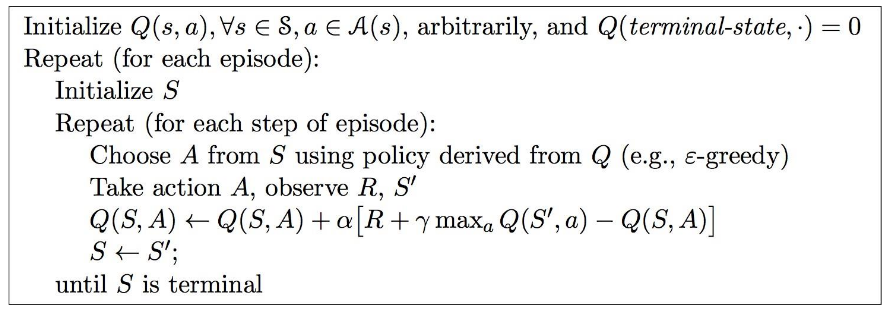
\includegraphics[width=0.7\textwidth]{images/L56.png}
    \caption{Algortimo Q-Learning}
    \label{fig:student_markov_chain}
\end{figure}

\begin{figure}[H]
    \centering
    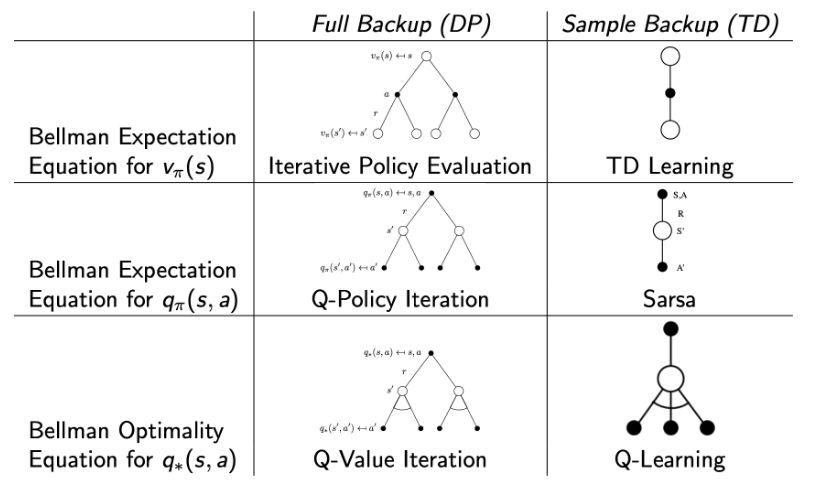
\includegraphics[width=0.7\textwidth]{images/L57.png}
    \caption{Relationship between DP and TD}
    \label{fig:student_markov_chain}
\end{figure}

\begin{figure}[H]
    \centering
    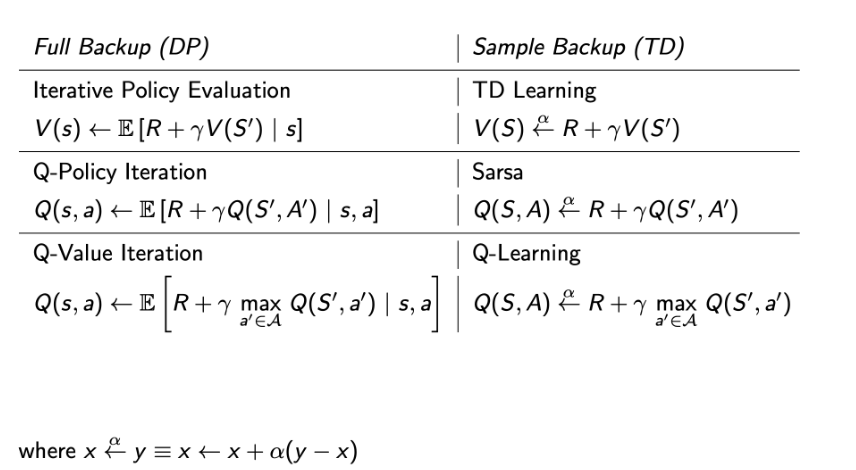
\includegraphics[width=0.7\textwidth]{images/L58.png}
    \caption{Relationship between DP and TD}
    \label{fig:student_markov_chain}
\end{figure}

\chapter{Value Function Approximation}

\section{Introduction and Motivation}
\subsection{Introduction}
In the previous lectures we represented value functions through a lookup table:
each state $s$ (or each pair $(s,a)$) has its own stored value.
This approach is simple but does not scale to large MDPs, because:

\begin{compactitemize}
    \item the number of states can be extremely large (for example Backgammon $10^{20}$ states; Go $10^{170}$ states);
    \item the state space can be continuous and therefore not enumerable;
    \item learning the value of each state individually requires an unrealistic amount of experience.
\end{compactitemize}

We therefore resort to a \textbf{parametric approximating function} that represents the value function with a reduced number of parameters:

\[
\hat{v}(s,\mathbf{w}) \approx v^\pi(s),
\qquad
\hat{q}(s,a,\mathbf{w}) \approx q^\pi(s,a).
\]

The goal is to generalize as much as possible from the observed states to those not yet visited.

\subsection{Large-Scale Reinforcement Learning}

Reinforcement Learning is applied to high-dimensional domains, such as:

\begin{compactitemize}
    \item complex games (Backgammon, Go);
    \item robotics and continuous control;
    \item industrial dynamical systems.
\end{compactitemize}

In such scenarios it is not possible to use a table.
A compact representation and an efficient update methodology therefore become fundamental.

In our context we assume \textbf{differentiable} approximators, so as to allow updates through gradient descent.

\subsection{Which Function Approximator?}

Unlike supervised learning, the data generated by an RL agent have some critical properties:

\begin{compactitemize}
    \item they are not i.i.d.;
    \item the distribution of visited states depends on the policy, which evolves over time;
    \item the targets themselves (such as TD targets) depend on the parameters and are not stationary.
\end{compactitemize}

These characteristics cause problems for gradient-based methods.
When the data are not i.i.d., the gradient estimate can become unstable: successive descent directions are not consistent and can produce oscillations or divergence.
This phenomenon is particularly evident with non-linear approximators, and it is one of the main reasons why techniques such as replay buffers, target networks and variance control methods are introduced.
\section{Gradient-Based Function Approximation}
\subsection{Gradient Descent (Recap)}

Given a differentiable objective $J(\mathbf{w})$, its gradient is:

\[
\nabla_{\mathbf{w}} J(\mathbf{w})
=
\begin{bmatrix}
\frac{\partial J}{\partial w_1} \\
\vdots \\
\frac{\partial J}{\partial w_n}
\end{bmatrix}.
\]

The gradient descent update is:

\[
\mathbf{w}_{t+1} = \mathbf{w}_t - \alpha \nabla_{\mathbf{w}} J(\mathbf{w}_t).
\]

In Reinforcement Learning we cannot compute the exact expectation of the gradient, so we use a sample estimator (SGD), which introduces noise but is computationally lighter.

\subsection{Value Function Approximation with SGD}

The goal is to minimize the squared error between the true value function and its approximation:

\[
J(\mathbf{w})
=
\mathbb{E}\left[
\left( v^\pi(S) - \hat{v}(S,\mathbf{w}) \right)^2
\right].
\]

The SGD update is:

\[
\Delta \mathbf{w}
=
\alpha
\left( v^\pi(S) - \hat{v}(S,\mathbf{w}) \right)
\nabla_{\mathbf{w}}\hat{v}(S,\mathbf{w}).
\]

Under ideal conditions this update converges to the minimum; in RL settings, the non-independence of the data requires particular attention to stability.

\subsection{Feature Vectors}

Each state is represented by a feature vector:

\[
\mathbf{x}(S)
=
\begin{bmatrix}
x_1(S) \\
\vdots \\
x_n(S)
\end{bmatrix}.
\]

Features provide a compact representation of the state.
Typical examples include: geometric distances, economic characteristics, structured descriptions of the configuration in a game.

\subsection{Linear Value Function Approximation}

A simple and stable approach consists of using a linear combination of features:

\[
\hat{v}(S,\mathbf{w})
=
\mathbf{x}(S)^T \mathbf{w}
=
\sum_{j=1}^{n} x_j(S) w_j.
\]

The corresponding objective to minimize is:

\[
J(\mathbf{w})
=
\mathbb{E}
\left[
\left( v^\pi(S) - \mathbf{x}(S)^T \mathbf{w} \right)^2
\right],
\]

which is convex in $\mathbf{w}$.
Consequently, SGD converges to the global minimum.
The update becomes:

\[
\Delta \mathbf{w}
=
\alpha
\left( v^\pi(S) - \hat{v}(S,\mathbf{w}) \right)
\mathbf{x}(S).
\]

\subsection{Table Lookup as Linear Approximation}

The tabular representation can be seen as a special case of linear approximation using indicator features:

\[
\mathbf{x}_{\text{table}}(S)
=
\begin{bmatrix}
\mathbf{1}(S = s_1) \\
\vdots \\
\mathbf{1}(S = s_n)
\end{bmatrix}.
\]

In this case, the vector $\mathbf{w}$ directly contains the values of the states:

\[
\hat{v}(S,\mathbf{w})
=
\mathbf{x}_{\text{table}}(S)^T \mathbf{w}.
\]

Although not scalable, this representation is the reference case and the conceptual starting point for more advanced feature engineering methods.
\section{Prediction with Function Approximation}

\subsection{Monte Carlo and TD Learning with Value Function Approximation}

In a Reinforcement Learning setting the true value function $v^\pi(s)$ is not available:
the agent receives only rewards and must therefore build a \textit{learning target} from experience.
The idea common to incremental prediction methods is to replace the true value function with an appropriate target, and to use this target within a gradient-based update:

\[
\Delta \mathbf{w}
=
\alpha \left( \text{target}_t - \hat{v}(S_t,\mathbf{w}) \right)
\nabla_{\mathbf{w}} \hat{v}(S_t,\mathbf{w}).
\]

In this section we analyse the targets used by Monte Carlo, TD(0) and TD($\lambda$).

\subsection{Monte Carlo with Value Function Approximation}

In the Monte Carlo method, the target for state $S_t$ is the \textbf{return} of the episode:

\[
G_t = \sum_{k=t}^{T-1} \gamma^{k-t} R_{k+1}.
\]

The return $G_t$ is an \textbf{unbiased} estimator of $v^\pi(s)$, although characterized by high variance.
After each episode we therefore obtain a series of training pairs:

\[
\langle S_1, G_1 \rangle, \langle S_2, G_2 \rangle, \dots, \langle S_T, G_T \rangle.
\]

For a linear approximator $\hat{v}(S,\mathbf{w}) = \mathbf{x}(S)^T \mathbf{w}$, the update becomes:

\[
\Delta \mathbf{w}
=
\alpha \left( G_t - \hat{v}(S_t,\mathbf{w}) \right) \mathbf{x}(S_t).
\]

Monte Carlo evaluation converges to a local optimum, even in the presence of non-linear approximation.

\subsection{TD(0) with Value Function Approximation}

The TD(0) method uses a target built \textit{online}, based on the next estimate of the value function.
The TD-target is:

\[
R_{t+1} + \gamma \hat{v}(S_{t+1}, \mathbf{w}).
\]

This target is \textbf{biased} with respect to $v^\pi(s)$, since it uses an approximate estimate, but it has lower variance and allows step-by-step updates.
The training data take the form:

\[
\langle S_1, R_2 + \gamma \hat{v}(S_2,\mathbf{w}) \rangle,
\dots,
\langle S_{T-1}, R_T \rangle.
\]

For the linear case, the update after each step is:

\[
\Delta \mathbf{w}
=
\alpha \left( R_{t+1} + \gamma \hat{v}(S_{t+1},\mathbf{w}) - \hat{v}(S_t,\mathbf{w}) \right)
\mathbf{x}(S_t)
=
\alpha \, \delta_t \, \mathbf{x}(S_t),
\]

where $\delta_t$ is the TD error.

For linear approximators, TD(0) converges close to the global optimum (the precision depends on the discount factor $\gamma$).

\subsection{TD($\lambda$) with Value Function Approximation}

The TD($\lambda$) method combines Monte Carlo and TD(0) through the parameter $\lambda \in [0,1]$.
It uses targets based on the \textit{$n$-step returns}, obtaining the \textbf{$\lambda$-return}:

\[
G_t^\lambda = (1-\lambda)
\sum_{n=1}^{\infty} \lambda^{n-1} G_t^{(n)}.
\]

The $\lambda$-return is also a \textbf{biased} estimator of the value function, but it generates on average more stable updates.
The training data are:

\[
\langle S_1, G_1^\lambda \rangle, \langle S_2, G_2^\lambda \rangle, \dots.
\]

\subsubsection{Forward View TD($\lambda$)}

The incremental update in the forward view is:

\[
\Delta \mathbf{w}
=
\alpha \left( G_t^\lambda - \hat{v}(S_t,\mathbf{w}) \right)
\nabla_{\mathbf{w}} \hat{v}(S_t,\mathbf{w})
=
\alpha \left( G_t^\lambda - \hat{v}(S_t,\mathbf{w}) \right)
\mathbf{x}(S_t).
\]

\subsubsection{Backward View TD($\lambda$)}

The backward view provides an equivalent but computationally more efficient formulation.
It introduces the vector of \textbf{eligibility traces}:

\[
E_t = \gamma \lambda E_{t-1} + \mathbf{x}(S_t),
\]

and the TD error:

\[
\delta_t = R_{t+1} + \gamma \hat{v}(S_{t+1},\mathbf{w}) - \hat{v}(S_t,\mathbf{w}).
\]

The parameter update is:

\[
\Delta \mathbf{w}
=
\alpha \, \delta_t \, E_t.
\]

The backward view is the one commonly used in implementations, since it requires neither waiting for the end of the episode nor storing multiple returns.
\section{Action-Value Function Approximation and Control}
\subsection{Action-Value Function Approximation}

The goal is not only to approximate the value function $v^\pi(s)$, but also the action-value function:

\[
\hat{q}(S,A,\mathbf{w}) \approx q^\pi(S,A).
\]

As in the case of the value function, an objective function based on the mean squared error is defined:

\[
J(\mathbf{w})
=
\mathbb{E}_\pi \left[
\left( q^\pi(S,A) - \hat{q}(S,A,\mathbf{w}) \right)^2
\right].
\]

The goal is to minimize this quantity through incremental gradient descent updates.
The stochastic gradient estimator provides the update:

\[
\Delta \mathbf{w}
=
\alpha \left( q^\pi(S_t,A_t) - \hat{q}(S_t,A_t,\mathbf{w}) \right)
\nabla_{\mathbf{w}} \hat{q}(S_t,A_t,\mathbf{w}).
\]

Since $q^\pi(s,a)$ is not directly observable, in RL methods this value is replaced by appropriate targets (Monte Carlo, TD, $\lambda$-return).

\subsection{Linear Action-Value Function Approximation}

To represent the action-value function through a linear approximator, joint state-action features are introduced:

\[
\mathbf{x}(S,A)
=
\begin{bmatrix}
x_1(S,A) \\
\vdots \\
x_n(S,A)
\end{bmatrix}.
\]

The estimated function takes the form:

\[
\hat{q}(S,A,\mathbf{w})
=
\mathbf{x}(S,A)^T \mathbf{w}
=
\sum_{j=1}^{n} x_j(S,A) w_j.
\]

The stochastic gradient descent update becomes:

\[
\nabla_{\mathbf{w}} \hat{q}(S_t,A_t,\mathbf{w}) = \mathbf{x}(S_t,A_t),
\]

\[
\Delta \mathbf{w}
=
\alpha \left( q^\pi(S_t,A_t) - \hat{q}(S_t,A_t,\mathbf{w}) \right)
\mathbf{x}(S_t,A_t).
\]

\subsection{Incremental Control Algorithms}

Analogously to policy evaluation, to learn the action-value function $q^\pi$ it is necessary to replace $q^\pi(S_t,A_t)$ with a target obtained from experience.
Depending on the method, Monte Carlo returns, TD targets, or $\lambda$-returns are used.

\subsubsection{Monte Carlo Control}

In the MC case, the target is the return:

\[
G_t = R_{t+1} + \gamma R_{t+2} + \cdots + \gamma^{T-t-1} R_T.
\]

The update becomes:

\[
\Delta \mathbf{w}
=
\alpha \left( G_t - \hat{q}(S_t,A_t,\mathbf{w}) \right)
\nabla_{\mathbf{w}} \hat{q}(S_t,A_t,\mathbf{w}).
\]

\subsubsection{TD(0) Control}

The TD(0) target for the action-value function is:

\[
R_{t+1} + \gamma \hat{q}(S_{t+1},A_{t+1},\mathbf{w}).
\]

The update is:

\[
\Delta \mathbf{w}
=
\alpha \left( R_{t+1} + \gamma \hat{q}(S_{t+1},A_{t+1},\mathbf{w}) -
\hat{q}(S_t,A_t,\mathbf{w}) \right)
\nabla_{\mathbf{w}} \hat{q}(S_t,A_t,\mathbf{w}).
\]

Defining the TD error for the action-value function:

\[
\delta_t
=
R_{t+1} + \gamma \hat{q}(S_{t+1},A_{t+1},\mathbf{w})
-
\hat{q}(S_t,A_t,\mathbf{w}),
\]

the update is written as:

\[
\Delta \mathbf{w} = \alpha \, \delta_t \, \nabla_{\mathbf{w}} \hat{q}(S_t,A_t,\mathbf{w}).
\]

\subsubsection{TD($\lambda$) Control}

For TD($\lambda$), the target is the action-value $\lambda$-return:

\[
q_t^\lambda.
\]

The forward view update is:

\[
\Delta \mathbf{w}
=
\alpha \left( q_t^\lambda - \hat{q}(S_t,A_t,\mathbf{w}) \right)
\nabla_{\mathbf{w}} \hat{q}(S_t,A_t,\mathbf{w}).
\]

\subsubsection{Backward View TD($\lambda$)}

The backward view form introduces the eligibility traces:

\[
E_t
=
\gamma \lambda E_{t-1}
+
\nabla_{\mathbf{w}} \hat{q}(S_t,A_t,\mathbf{w}),
\]

and uses the TD error:

\[
\delta_t
=
R_{t+1}
+
\gamma \hat{q}(S_{t+1},A_{t+1},\mathbf{w})
-
\hat{q}(S_t,A_t,\mathbf{w}).
\]

The parameter update is:

\[
\Delta \mathbf{w}
=
\alpha \, \delta_t \, E_t.
\]

This method is equivalent to the forward view but much more computationally efficient.

\section{Stability, Convergence and Batch Methods}

\subsection{Convergence of Prediction Algorithms}

In the case of policy evaluation with an approximate value function, the convergence of the various algorithms depends on:

\begin{compactitemize}
    \item the type of method (MC, TD(0), TD($\lambda$), etc.);
    \item the type of approximator (linear or non-linear);
    \item the on-policy vs off-policy scenario.
\end{compactitemize}

In general:

\begin{compactitemize}
    \item \textbf{Monte Carlo} with an approximate function (even non-linear) corresponds to a supervised regression problem with fixed targets (the returns $G_t$). In this case there are good guarantees of convergence to a local optimum of the error function;
    \item \textbf{TD(0)} with a \textbf{linear} approximator and \textbf{on-policy} converges to the projected fixed point of the Bellman operator (convergence ``close'' to the optimum, depending on $\gamma$);
    \item \textbf{TD(0)} (and TD($\lambda$)) with a \textbf{non-linear} approximate function or in an \textbf{off-policy} setting have in general no convergence guarantees: they may converge in practice, but there are counterexamples in which they diverge.
\end{compactitemize}

In the slides, the notation ``$x$'' indicates precisely the cases in which \textbf{there are no theoretical convergence guarantees}, even though the algorithm may behave well empirically.

\subsection{Gradient TD Learning}

Standard TD algorithms (such as TD(0), TD($\lambda$)) do not correspond to the gradient descent of an explicit objective function.
In particular, the TD update:

\[
\Delta \mathbf{w}
=
\alpha
\left( R_{t+1} + \gamma \hat{v}(S_{t+1},\mathbf{w}) - \hat{v}(S_t,\mathbf{w}) \right)
\nabla_{\mathbf{w}} \hat{v}(S_t,\mathbf{w})
\]

is not in general the gradient of a functional $J(\mathbf{w})$.

This is the reason why:

\begin{compactitemize}
    \item TD can diverge with a non-linear approximate function;
    \item TD can diverge in an off-policy scenario, even with a linear approximator.
\end{compactitemize}

\textbf{Gradient TD} algorithms were introduced precisely to solve this problem:
they approximate the true gradient descent of a well-defined error measure (for example the \emph{projected Bellman error}), introducing auxiliary weights and specifically designed updates.
In this way they recover convergence guarantees in settings where standard TD can diverge.

\subsection{Convergence of Control Algorithms}

For control (learning an optimal policy), the situation is even more delicate:

\begin{compactitemize}
    \item with a tabular representation and on-policy algorithms (e.g. tabular SARSA) there are guarantees of convergence to the optimal policy (under suitable conditions on exploration and step-size);
    \item with a \textbf{linear} approximate function and on-policy algorithms some guarantees can be obtained, but much weaker ones;
    \item with a \textbf{non-linear} approximate function (e.g. deep networks) and in particular in off-policy settings (e.g. Q-learning + replay) there are no general theoretical convergence guarantees: the behaviour is driven mainly by empirical experience and by stabilization techniques.
\end{compactitemize}

For this reason, the design of stable control algorithms with function approximation is an active research area.

\subsection{Batch Reinforcement Learning}

Incremental gradient descent algorithms update $\mathbf{w}$ step by step during the interaction.
These methods are simple to implement, but \textbf{not very sample-efficient}: each transition is used only once and then discarded.

\textbf{Batch} methods take a different perspective:

\begin{compactitemize}
    \item a fixed dataset of experience is collected;
    \item we look for the value function that best approximates the targets on that dataset.
\end{compactitemize}

In other words, given a set of \texttt{<state, target>} pairs obtained from experience, we look for the function $v(s,\mathbf{w})$ that \textbf{best fits} these data in the least-squares sense.

\subsection{Least Squares Prediction}

Suppose we have an approximator $ \hat{v}(s,\mathbf{w}) \approx v^\pi(s)$ and a dataset of experience:

\[
\mathcal{D} = \{ \langle s_1, v_1^\pi \rangle, \langle s_2, v_2^\pi \rangle, \dots, \langle s_T, v_T^\pi \rangle \},
\]

where $v_t^\pi$ is a target for the value in $s_t$ (ideally $v^\pi(s_t)$, or an estimate such as the Monte Carlo return or a $\lambda$-return).

The question is: \textit{which parameters $\mathbf{w}$ produce the best approximation of these targets?}

Least-squares algorithms look for the vector $\mathbf{w}$ that minimizes:

\[
L_{LS}(\mathbf{w})
=
\sum_{t=1}^{T} \left( v_t^\pi - \hat{v}(s_t,\mathbf{w}) \right)^2
=
\mathbb{E}_{\mathcal{D}} \left[ \left( v^\pi - \hat{v}(s,\mathbf{w}) \right)^2 \right],
\]

where the expectation is computed with respect to the empirical distribution of the data in the dataset $\mathcal{D}$.

\section{Stochastic Gradient Descent with Experience Replay}

A simple way to approximate the least-squares solution, reusing past experience, is the use of \textbf{experience replay}:

\begin{compactitemize}
    \item a dataset $\mathcal{D} = \{ \langle s_t, v_t^\pi \rangle \}$ is built from the observed transitions (for example using MC returns, TD($\lambda$), etc. as targets);
    \item \texttt{<state, target>} pairs are randomly sampled from the dataset to break the temporal correlations;
    \item an SGD step is applied to each sample.
\end{compactitemize}

Formally:

\begin{compactitemize}
    \item we draw $\langle s, v^\pi \rangle \sim \mathcal{D}$;
    \item we update
    \[
    \Delta \mathbf{w}
    =
    \alpha \left( v^\pi - \hat{v}(s,\mathbf{w}) \right)
    \nabla_{\mathbf{w}} \hat{v}(s,\mathbf{w}).
    \]
\end{compactitemize}

By repeating this procedure, SGD converges to the least-squares solution:

\[
\mathbf{w}^\pi = \arg\min_{\mathbf{w}} L_{LS}(\mathbf{w}).
\]

The central idea is that experience replay:

\begin{compactitemize}
    \item reuses the same transitions many times;
    \item reduces the correlation between samples, bringing the setting closer to the i.i.d. one;
    \item stabilizes the training of the approximating function.
\end{compactitemize}

\subsection{Experience Replay in Deep Q-Networks (DQN)}

In the case of Deep Q-Networks (DQN), experience replay is combined with the use of \textbf{fixed Q-targets} to stabilize training.

The scheme is the following:

\begin{compactitemize}
    \item the agent executes an action $a_t$ according to an $\epsilon$-greedy policy with respect to $Q(s,a;\mathbf{w})$;
    \item the transition $(s_t, a_t, r_{t+1}, s_{t+1})$ is inserted into a replay memory $\mathcal{D}$;
    \item periodically, a mini-batch of transitions $(s,a,r,s')$ is sampled from $\mathcal{D}$;
    \item for each sample the Q-learning target is computed using a \emph{fixed} weight vector $\mathbf{w}_{old}$:
    \[
    y = r + \gamma \max_{a'} Q(s',a'; \mathbf{w}_{old});
    \]
    \item the MSE between the current Q-network $Q(s,a;\mathbf{w})$ and the target $y$ is minimized:
    \[
    \mathcal{L}(\mathbf{w})
    =
    \mathbb{E}_{(s,a,r,s') \sim \mathcal{D}}
    \left[
    \left( y - Q(s,a; \mathbf{w}) \right)^2
    \right];
    \]
    \item the parameters $\mathbf{w}$ are updated with a variant of stochastic gradient descent.
\end{compactitemize}

The use of $\mathbf{w}_{old}$ (``frozen'' parameters) for computing the target is crucial:

\begin{compactitemize}
    \item it prevents the target from changing too quickly while the weights are updated;
    \item it makes the optimization more similar to a supervised regression problem with almost fixed targets;
    \item it contributes decisively to the stability of training, especially in the presence of deep approximating functions and non-i.i.d. data.
\end{compactitemize}

By combining:

\begin{compactitemize}
    \item replay buffer (to decorrelate the data and reuse the transitions);
    \item fixed target network (to make the target more stable);
\end{compactitemize}

DQN manages to effectively apply the ideas of Q-learning in the presence of non-linear approximation through deep neural networks, mitigating many of the instability problems discussed previously.

\chapter{Policy-Based Methods}
\section{Introduction}
Nel capitolo precedente abbiamo visto come approssimare la \emph{state-value function} e la \emph{action-value function} utilizzando un insieme di parametri $w$. Nel contesto dei \emph{value-based methods}, la policy che viene appresa è \textbf{implicita}, in quanto viene derivata direttamente dalla value function (ad esempio selezionando l’azione che massimizza $Q(s,a)$).

In questo capitolo, invece, andiamo a parametrizzare direttamente la policy. In particolare, modelliamo la policy come una distribuzione di probabilità sulle azioni dato lo stato:
\[
\pi_w(s,a) = \mathbb{P}[a \mid s,w],
\]
e ci concentriamo nuovamente su \emph{model-free reinforcement learning}.

È utile chiarire fin da subito la distinzione tra i principali approcci in reinforcement learning:
\begin{compactitemize}
    \item \textbf{Value-Based}: apprendono una value function; la policy è implicita.
    \item \textbf{Policy-Based}: non apprendono alcuna value function, ma modellano direttamente una policy parametrizzata.
    \item \textbf{Actor-Critic}: apprendono sia una policy (actor) sia una value function (critic); rappresentano lo stato dell’arte.
\end{compactitemize}

I \emph{policy-based methods} presentano diversi vantaggi. In primo luogo, mostrano migliori proprietà di convergenza rispetto ai value-based methods. Inoltre, risultano particolarmente efficaci in spazi delle azioni continui o ad alta dimensionalità. Un aspetto fondamentale è che questi metodi possono apprendere \textbf{stochastic policies}, che in molti problemi risultano necessarie per ottenere un comportamento ottimale.

Esistono tuttavia anche degli svantaggi. In generale, i policy-based methods convergono tipicamente a un \emph{local optimum} e non garantiscono il raggiungimento di un \emph{global optimum}. Inoltre, la policy evaluation tramite campionamento è spesso inefficiente e caratterizzata da high variance, rendendo il processo di apprendimento più instabile.
\subsection{Esempi}
\subsubsection{Primo esempio}
Un primo esempio che chiarisce la necessità di stochastic policies è il gioco a due giocatori di \emph{rock-paper-scissors}. Considerando versioni iterate del gioco, una deterministic policy è facilmente exploitable dall’avversario, mentre una uniform random policy è ottimale e corrisponde a un \emph{Nash equilibrium}. Questo tipo di comportamento emerge naturalmente con un approccio policy-based.
\subsubsection{Secondo esempio}
Un secondo esempio è quello dell’\textbf{aliased gridworld}. In questo scenario, l’agente non è in grado di distinguere completamente alcuni stati (gli stati grigi), a causa di osservazioni ambigue. Consideriamo feature del tipo:
\[
\mathbf{x}(s,a) = 1(\text{wall to N},\, a = \text{move E}),
\]
per tutte le direzioni $N,E,S,W$.

Un approccio value-based utilizza una approssimazione della action-value function:
\[
Q_w(s,a) = f(\mathbf{x}(s,a), w),
\]
da cui deriva una policy quasi-deterministic.

Sotto condizioni di aliasing, una optimal deterministic policy finirà per selezionare la stessa azione in tutti gli stati grigi, muovendosi sempre verso East oppure sempre verso West. In entrambi i casi, l’agente può rimanere bloccato nel corridoio e non raggiungere mai lo stato obiettivo. I value-based methods tendono infatti ad apprendere near-deterministic policies, che in presenza di aliasing risultano subottimali.

Un approccio policy-based, invece, parametrizza direttamente la policy:
\[
\pi_w(s,a) = g(\mathbf{x}(s,a), w),
\]
e può rappresentare una optimal stochastic policy. In particolare, negli stati grigi la policy ottimale assegna probabilità uguali alle azioni \emph{move East} e \emph{move West}:
\[
\pi_w(\text{wall to N and S}, \text{move E}) = 0.5, \qquad
\pi_w(\text{wall to N and S}, \text{move W}) = 0.5.
\]
In questo modo, con alta probabilità l’agente raggiunge il goal state in pochi passi. Questo esempio mostra come i policy-based methods siano in grado di apprendere optimal stochastic policies in scenari in cui i value-based methods falliscono.
\section{Policy-Base Methods}
\subsection{Policy Objective Functions}

L’obiettivo dei \emph{policy-based methods} è trovare i parametri $\mathbf{w}$ che rendono la policy $\pi_{\mathbf{w}}(s,a)$ la migliore possibile. Il problema centrale diventa quindi definire una funzione obiettivo che misuri la qualità di una policy.

Nei contesti \emph{episodic}, una scelta naturale consiste nel valore atteso dello stato iniziale $s_1$, noto come \emph{start value}:
\[
J_1(\mathbf{w}) = V^{\pi_{\mathbf{w}}}(s_1) = \mathbb{E}_{\pi_{\mathbf{w}}}[v_1].
\]
In questo caso, massimizzare $J_1(\mathbf{w})$ equivale a massimizzare il ritorno atteso a partire dall’inizio dell’episodio.

Nei contesti \emph{continuing}, dove non esiste uno stato iniziale privilegiato, è comune utilizzare una misura media sulle distribuzioni stazionarie. Una possibilità è definire l’\emph{average value}:
\[
J_{\text{avV}}(\mathbf{w}) =
\sum_s d_{\pi_{\mathbf{w}}}(s)\, V^{\pi_{\mathbf{w}}}(s),
\]
dove $d_{\pi_{\mathbf{w}}}(s)$ rappresenta la \emph{stationary distribution} della catena di Markov indotta dalla policy $\pi_{\mathbf{w}}$.

Un’alternativa, spesso più utilizzata in pratica, è l’\emph{average reward per time-step}:
\[
J_{\text{avR}}(\mathbf{w}) =
\sum_s d_{\pi_{\mathbf{w}}}(s)\, 
\sum_a \pi_{\mathbf{w}}(s,a)\, R_s^a.
\]
Questa formulazione misura direttamente il reward medio ottenuto dall’agente nel lungo periodo e risulta particolarmente adatta a problemi continui.

\subsection{Policy Optimisation}

Una volta definita la funzione obiettivo $J(\mathbf{w})$, il reinforcement learning policy-based può essere visto come un problema di ottimizzazione:
\[
\max_{\mathbf{w}} J(\mathbf{w}).
\]
Esistono diversi approcci per affrontare questo problema. Alcuni metodi non utilizzano il gradiente della funzione obiettivo, come ad esempio \emph{hill climbing}, \emph{simplex / amoeba / Nelder-Mead} e \emph{genetic algorithms}. Questi metodi sono concettualmente semplici, ma spesso poco efficienti in spazi dei parametri elevati.

Una maggiore efficienza può essere ottenuta sfruttando informazioni di gradiente. Tra i metodi basati sul gradiente rientrano il \emph{gradient descent}, il \emph{conjugate gradient} e i metodi \emph{quasi-Newton}. In questo capitolo ci concentriamo in particolare sul gradient descent e su estensioni che sfruttano la struttura sequenziale del reinforcement learning.

\subsection{Policy Gradient}

I \emph{policy gradient methods} assumono che $J(\mathbf{w})$ sia una funzione differenziabile rispetto ai parametri della policy. L’idea è quella di cercare un massimo locale di $J(\mathbf{w})$ muovendosi nella direzione del gradiente.

Il gradiente della policy è definito come:
\[
\nabla_{\mathbf{w}} J(\mathbf{w}) =
\begin{bmatrix}
\frac{\partial J(\mathbf{w})}{\partial w_1} \\
\vdots \\
\frac{\partial J(\mathbf{w})}{\partial w_n}
\end{bmatrix}.
\]
I parametri vengono aggiornati seguendo la direzione di massima crescita della funzione obiettivo:
\[
\Delta \mathbf{w} = \alpha \nabla_{\mathbf{w}} J(\mathbf{w}),
\]
dove $\alpha$ è un parametro di \emph{step-size} che controlla l’ampiezza dell’aggiornamento.

Questa regola di aggiornamento costituisce il principio fondamentale dei policy gradient methods: invece di stimare una value function e derivarne una policy, l’agente modifica direttamente i parametri della policy in modo da aumentare il valore atteso del criterio di performance scelto.

\subsection{Score Function}

Per calcolare in modo analitico il \emph{policy gradient}, assumiamo che la policy $\pi_{\mathbf{w}}(s,a)$ sia differenziabile rispetto ai parametri $\mathbf{w}$ in tutti i punti in cui è non nulla, e che siamo in grado di calcolare il gradiente
\[
\nabla_{\mathbf{w}} \pi_{\mathbf{w}}(s,a).
\]
Un’idea fondamentale è quella di utilizzare i \emph{likelihood ratios}, che si basano sulla seguente identità:
\[
\nabla_{\mathbf{w}} \pi_{\mathbf{w}}(s,a)
= \pi_{\mathbf{w}}(s,a)\, \nabla_{\mathbf{w}} \log \pi_{\mathbf{w}}(s,a).
\]
Questa formula si ottiene applicando semplicemente la regola della derivata del logaritmo:
\[
\nabla_{\mathbf{w}} \log \pi_{\mathbf{w}}(s,a)
= \frac{1}{\pi_{\mathbf{w}}(s,a)}\, \nabla_{\mathbf{w}} \pi_{\mathbf{w}}(s,a),
\]
e moltiplicando entrambi i membri per $\pi_{\mathbf{w}}(s,a)$.

Il termine
\[
\nabla_{\mathbf{w}} \log \pi_{\mathbf{w}}(s,a)
\]
viene chiamato \emph{score function}. L’uso della score function è particolarmente conveniente perché le espressioni del tipo
\[
\mathbb{E}_{\pi_{\mathbf{w}}}\big[\nabla_{\mathbf{w}} \log \pi_{\mathbf{w}}(s,a)\,\cdot(\cdot)\big]
\]
sono molto più semplici da trattare rispetto alle derivate dirette della policy. Inoltre, la score function ha una struttura intuitiva e spesso ammette una forma chiusa per policy comuni (ad esempio softmax e Gaussian policy), come vedremo tra poco.

\subsection{Linear Softmax Policy}

Consideriamo ora una \emph{softmax policy} per il caso di azioni discrete. Usiamo un vettore di feature $\mathbf{x}(s,a)$ che descrive la coppia stato-azione e un vettore di parametri $\mathbf{w}$. Assegniamo a ciascuna azione un \emph{peso} dato da una combinazione lineare:
\[
\mathbf{x}(s,a)^\top \mathbf{w}.
\]
La policy softmax definisce quindi la probabilità di selezionare un’azione proporzionale all’esponenziale di questo peso:
\[
\pi_{\mathbf{w}}(s,a)
= \frac{\exp\big(\mathbf{x}(s,a)^\top \mathbf{w}\big)}
       {\sum_{a'} \exp\big(\mathbf{x}(s,a')^\top \mathbf{w}\big)}.
\]

Per questa policy, la score function assume una forma particolarmente elegante:
\[
\nabla_{\mathbf{w}} \log \pi_{\mathbf{w}}(s,a)
= \mathbf{x}(s,a) - \mathbb{E}_{\pi_{\mathbf{w}}}\big[\mathbf{x}(s,\cdot)\big],
\]
dove
\[
\mathbb{E}_{\pi_{\mathbf{w}}}\big[\mathbf{x}(s,\cdot)\big]
= \sum_{a'} \pi_{\mathbf{w}}(s,a')\, \mathbf{x}(s,a')
\]
è la media delle feature pesata dalla policy.

Questa espressione ha un’interpretazione molto intuitiva: la score function è la differenza tra le feature dell’azione effettivamente scelta e le feature medie delle azioni che avremmo potuto scegliere in quello stato. Se una certa combinazione di feature si manifesta più spesso del previsto e produce buon reward, il gradiente spingerà la policy ad aumentare la probabilità di tali azioni. Viceversa, se produce cattivo reward, il gradiente ne ridurrà la probabilità.

\subsection{Gaussian Policy}

Nel caso di spazi delle azioni continui, una scelta naturale è una \emph{Gaussian policy}. Consideriamo il caso in cui l’azione $a \in \mathbb{R}$ sia un valore reale e definiremo la media come una combinazione lineare di feature dello stato:
\[
\mu(s) = \mathbf{x}(s)^\top \mathbf{w}.
\]
La varianza $\sigma^2$ può essere assunta costante oppure anch’essa parametrizzata; nel caso più semplice, supponiamo $\sigma^2$ fissata.

La policy è allora definita come:
\[
\pi_{\mathbf{w}}(a \mid s) = \mathcal{N}\big(a;\, \mu(s), \sigma^2\big),
\]
ovvero una distribuzione Gaussiana con media $\mu(s)$ e varianza $\sigma^2$.

La log-policy è:
\[
\log \pi_{\mathbf{w}}(a \mid s)
= -\frac{(a - \mu(s))^2}{2\sigma^2} - \log\big(\sqrt{2\pi}\,\sigma\big).
\]
Derivando rispetto a $\mathbf{w}$, otteniamo la score function:
\[
\nabla_{\mathbf{w}} \log \pi_{\mathbf{w}}(a \mid s)
= \frac{a - \mu(s)}{\sigma^2}\, \mathbf{x}(s).
\]
Anche qui l’interpretazione è chiara: se l’azione $a$ è maggiore della media $\mu(s)$, il termine $(a - \mu(s))$ è positivo e il gradiente spinge la media verso l’alto in direzione di $\mathbf{x}(s)$; se è minore, la media viene spinta verso il basso. In presenza di un buon reward, questo meccanismo fa sì che la policy si adatti in modo da spostare la distribuzione delle azioni verso quei valori che hanno portato a ritorni più alti. 

Se si parametrizza anche la varianza, si può derivare una score function aggiuntiva rispetto ai parametri che controllano $\sigma^2$, in modo da aumentare la varianza quando le azioni lontane dalla media producono reward utili, e ridurla quando è preferibile concentrarsi in intorno alla media appresa.

\subsection{Policy Gradient Theorem: One-Step MDPs}

Per introdurre il \emph{policy gradient theorem}, iniziamo da un caso semplice: un \emph{one-step MDP}. In questo scenario:
\begin{compactitemize}
    \item si parte da uno stato $s \sim d(s)$, dove $d(s)$ è una distribuzione di probabilità sugli stati;
    \item si esegue una sola azione $a \sim \pi_{\mathbf{w}}(s,\cdot)$;
    \item l’episodio termina immediatamente con un reward $r = \mathcal{R}_s^a$.
\end{compactitemize}
Definiamo l’obiettivo come il valore atteso del reward:
\[
J(\mathbf{w}) = \mathbb{E}_{\pi_{\mathbf{w}}}[r]
= \sum_{s \in \mathcal{S}} d(s) \sum_{a \in \mathcal{A}} \pi_{\mathbf{w}}(s,a)\, \mathcal{R}_s^a.
\]

Per calcolare il gradiente, utilizziamo l’identità della score function:
\[
\nabla_{\mathbf{w}} \pi_{\mathbf{w}}(s,a)
= \pi_{\mathbf{w}}(s,a)\, \nabla_{\mathbf{w}} \log \pi_{\mathbf{w}}(s,a).
\]
Otteniamo:
\[
\begin{aligned}
\nabla_{\mathbf{w}} J(\mathbf{w})
&= \sum_{s} d(s) \sum_{a} \nabla_{\mathbf{w}} \pi_{\mathbf{w}}(s,a)\, \mathcal{R}_s^a \\
&= \sum_{s} d(s) \sum_{a} \pi_{\mathbf{w}}(s,a)\, \nabla_{\mathbf{w}} \log \pi_{\mathbf{w}}(s,a)\, \mathcal{R}_s^a \\
&= \mathbb{E}_{\pi_{\mathbf{w}}}\big[\nabla_{\mathbf{w}} \log \pi_{\mathbf{w}}(s,a)\, r\big].
\end{aligned}
\]
Questa è la forma base del \emph{likelihood ratio policy gradient}: il gradiente dell’obiettivo è l’aspettativa della score function pesata dal reward osservato. In pratica, questo ci dice che possiamo stimare il gradiente campionando $(s,a,r)$ dalla policy corrente e moltiplicando la score function per il reward.

\subsection{Policy Gradient Theorem}

Il \emph{policy gradient theorem} generalizza il risultato precedente a MDP multi-step, in cui gli episodi possono durare molti time-step. L’idea è simile: invece di usare il reward immediato $r$, il termine che compare nel gradiente è il valore a lungo termine dell’azione, ovvero la action-value function $Q^{\pi}(s,a)$.

In modo informale, l’obiettivo $J(\mathbf{w})$ può essere definito come uno dei seguenti:
\begin{compactitemize}
    \item start state objective $J_1(\mathbf{w}) = V^{\pi_{\mathbf{w}}}(s_1)$;
    \item average reward objective $J_{\text{avR}}(\mathbf{w})$;
    \item average value objective $J_{\text{avV}}(\mathbf{w})$.
\end{compactitemize}
Il teorema afferma che, per qualsiasi policy differenziabile $\pi_{\mathbf{w}}(s,a)$ e per qualsiasi di questi obiettivi, il gradiente assume la forma:
\[
\nabla_{\mathbf{w}} J(\mathbf{w})
= \mathbb{E}_{\pi_{\mathbf{w}}}\big[\nabla_{\mathbf{w}} \log \pi_{\mathbf{w}}(s,a)\, Q^{\pi_{\mathbf{w}}}(s,a)\big].
\]

Questa espressione è il cuore dei policy gradient methods. Essa ci dice che, per migliorare la policy:
\begin{compactitemize}
    \item aumentiamo la probabilità delle azioni che in media portano a un $Q^{\pi}(s,a)$ elevato;
    \item riduciamo la probabilità delle azioni con $Q^{\pi}(s,a)$ basso.
\end{compactitemize}
Il tutto avviene attraverso la score function $\nabla_{\mathbf{w}} \log \pi_{\mathbf{w}}(s,a)$, che traduce l’informazione sul “quanto è buona” un’azione (via $Q^{\pi}(s,a)$) in un aggiornamento diretto dei parametri $\mathbf{w}$ della policy.

\subsection{REINFORCE: Monte Carlo Policy Gradient}

Sulla base del policy gradient theorem, possiamo aggiornare i parametri della policy utilizzando \emph{stochastic gradient ascent}. L’idea è quella di stimare il gradiente di $J(\mathbf{w})$ campionando traiettorie generate dalla policy corrente e utilizzando tali campioni per effettuare aggiornamenti incrementali.

Dal policy gradient theorem sappiamo che:
\[
\nabla_{\mathbf{w}} J(\mathbf{w})
= \mathbb{E}_{\pi_{\mathbf{w}}}\big[\nabla_{\mathbf{w}} \log \pi_{\mathbf{w}}(s,a)\, Q^{\pi}(s,a)\big].
\]
Poiché la action-value function $Q^{\pi}(s,a)$ non è nota, possiamo utilizzare il \emph{return} Monte Carlo $G_t$ come stima non distorta di $Q^{\pi}(s_t,a_t)$. In particolare, $G_t$ rappresenta la somma dei reward futuri osservati a partire dal time-step $t$, ed è una realizzazione campionata del valore atteso a lungo termine.

Sostituendo $Q^{\pi}(s_t,a_t)$ con $G_t$, otteniamo una stima non distorta del gradiente:
\[
\nabla_{\mathbf{w}} J(\mathbf{w})
\approx
\nabla_{\mathbf{w}} \log \pi_{\mathbf{w}}(s_t,a_t)\, G_t.
\]
L’aggiornamento dei parametri viene quindi effettuato tramite stochastic gradient ascent:
\[
\Delta \mathbf{w}_t
= \alpha \nabla_{\mathbf{w}} \log \pi_{\mathbf{w}}(s_t,a_t)\, G_t,
\]
dove $\alpha$ è il learning rate.

Questo metodo è noto come \emph{REINFORCE} ed è un algoritmo \emph{Monte Carlo policy gradient}, in quanto utilizza traiettorie complete per stimare il return. REINFORCE è teoricamente corretto e semplice da implementare, ma soffre in genere di un’elevata varianza delle stime del gradiente.

L’algoritmo REINFORCE può essere descritto come segue:

\begin{enumerate}
    \item Inizializza i parametri della policy $\mathbf{w}$ arbitrariamente.
    \item Ripeti per ogni episodio:
    \begin{enumerate}
        \item Genera un episodio seguendo la policy $\pi_{\mathbf{w}}$:
        \[
        s_0, a_0, r_1, s_1, a_1, r_2, \dots, s_T
        \]
        \item Per ogni time-step $t = 0,1,\dots,T-1$:
        \begin{enumerate}
            \item Calcola il return:
            \[
            G_t = \sum_{k=0}^{T-t-1} \gamma^k r_{t+k+1}.
            \]
            \item Aggiorna i parametri della policy:
            \[
            \mathbf{w} \leftarrow \mathbf{w}
            + \alpha \nabla_{\mathbf{w}} \log \pi_{\mathbf{w}}(s_t,a_t)\, G_t.
            \]
        \end{enumerate}
    \end{enumerate}
\end{enumerate}

In sintesi, REINFORCE aumenta la probabilità delle azioni che hanno prodotto un alto return e riduce la probabilità delle azioni che hanno prodotto un basso return. Poiché utilizza il return completo $G_t$, l’algoritmo fornisce una stima non distorta del gradiente, ma con varianza elevata, motivo per cui nelle sezioni successive introdurremo il concetto di \emph{baseline} e il passaggio agli approcci \emph{actor-critic}.

\section{Actor-Critic Methods}

I \emph{Monte-Carlo policy gradient methods}, come REINFORCE, forniscono una stima non distorta del gradiente ma soffrono di \emph{high variance}, perché utilizzano il return completo $G_t$. Per ridurre la varianza pur mantenendo un aggiornamento online, si introduce la famiglia degli \emph{actor-critic methods}.

L’idea chiave è separare due ruoli distinti:
\begin{compactitemize}
    \item \textbf{Actor}: rappresenta e aggiorna la policy $\pi_\theta(s,a)$;
    \item \textbf{Critic}: valuta la policy stimando una value function.
\end{compactitemize}

Di conseguenza, un algoritmo actor-critic mantiene \textbf{due insiemi di parametri}:
\begin{compactitemize}
    \item $\theta$: parametri della policy (actor);
    \item $\mathbf{w}$: parametri della value function (critic).
\end{compactitemize}

\subsection{Actor-Critic Policy Gradient}

Negli actor-critic methods, il critic fornisce una stima di $Q^\pi(s,a)$, che viene utilizzata dall’actor per aggiornare la policy. In questo modo, il policy gradient non utilizza più il return Monte Carlo, ma una stima approssimata del valore dell’azione.

Il policy gradient theorem diventa quindi:
\[
\nabla_\theta J(\theta)
\approx
\mathbb{E}_{\pi_\theta}
\big[
\nabla_\theta \log \pi_\theta(s,a)\, Q_{\mathbf{w}}(s,a)
\big],
\]
dove $Q_{\mathbf{w}}(s,a)$ è l’approssimazione della action-value function fornita dal critic.

In pratica, l’aggiornamento dell’actor è:
\[
\Delta \theta
= \alpha \nabla_\theta \log \pi_\theta(s_t,a_t)\, Q_{\mathbf{w}}(s_t,a_t),
\]
dove $\alpha$ è il learning rate dell’actor.

Poiché il critic fornisce solo una stima del valore, questi metodi seguono un \emph{approximate policy gradient}. Tuttavia, il notevole vantaggio è una drastica riduzione della varianza rispetto ai metodi Monte Carlo.

\subsection{Estimating the Action-Value Function (Critic)}

Il ruolo del critic è risolvere un problema noto: la \emph{policy evaluation}. Data una policy $\pi_\theta$, il critic deve rispondere alla domanda:
\[
\text{How good is the current policy?}
\]

Questo problema è stato già affrontato in precedenza e può essere risolto con diversi metodi:
\begin{compactitemize}
    \item Monte-Carlo policy evaluation;
    \item Temporal-Difference learning;
    \item TD($\lambda$);
    \item Least-squares policy evaluation.
\end{compactitemize}

Negli actor-critic methods online, la scelta più comune è utilizzare \emph{TD learning}, poiché permette aggiornamenti incrementali a ogni time-step.

\subsection{Action-Value Actor-Critic}

Consideriamo ora una forma specifica di actor-critic: l’\emph{Action-Value Actor-Critic}. In questo caso, il critic approssima direttamente la action-value function:
\[
Q_{\mathbf{w}}(s,a).
\]

Assumiamo una approssimazione lineare:
\[
Q_{\mathbf{w}}(s,a) = \mathbf{x}(s,a)^\top \mathbf{w},
\]
dove $\mathbf{x}(s,a)$ è un vettore di feature.

Il critic viene aggiornato tramite \emph{linear TD(0)}. Definiamo l’errore di TD:
\[
\delta_t
= r_{t+1}
+ \gamma Q_{\mathbf{w}}(s_{t+1},a_{t+1})
- Q_{\mathbf{w}}(s_t,a_t).
\]

L’aggiornamento dei parametri del critic è:
\[
\mathbf{w}
\leftarrow
\mathbf{w}
+ \beta\, \delta_t\, \mathbf{x}(s_t,a_t),
\]
dove $\beta$ è il learning rate del critic.

L’actor aggiorna invece i parametri della policy seguendo il policy gradient, utilizzando la stima del critic:
\[
\theta
\leftarrow
\theta
+ \alpha \nabla_\theta \log \pi_\theta(s_t,a_t)\, Q_{\mathbf{w}}(s_t,a_t).
\]

\subsection{Action-Value Actor-Critic Algorithm}

L’algoritmo completo può essere riassunto come segue:

\begin{enumerate}
    \item Inizializza i parametri della policy $\theta$ e del critic $\mathbf{w}$.
    \item Osserva lo stato iniziale $s$.
    \item Ripeti per ogni time-step:
    \begin{enumerate}
        \item Seleziona un’azione $a \sim \pi_\theta(\cdot \mid s)$.
        \item Osserva reward $r$ e stato successivo $s'$.
        \item Seleziona la prossima azione $a' \sim \pi_\theta(\cdot \mid s')$.
        \item Calcola la TD error:
        \[
        \delta = r + \gamma Q_{\mathbf{w}}(s',a') - Q_{\mathbf{w}}(s,a).
        \]
        \item Aggiorna il critic:
        \[
        \mathbf{w} \leftarrow \mathbf{w} + \beta\, \delta\, \mathbf{x}(s,a).
        \]
        \item Aggiorna l’actor:
        \[
        \theta \leftarrow \theta + \alpha\, \nabla_\theta \log \pi_\theta(s,a)\, Q_{\mathbf{w}}(s,a).
        \]
        \item Poni $s \leftarrow s'$, $a \leftarrow a'$.
    \end{enumerate}
\end{enumerate}

In sintesi, l’actor-critic framework combina i vantaggi dei policy-based methods (apprendimento diretto della policy) con quelli dei value-based methods (bassa varianza grazie al bootstrapping), rappresentando uno dei paradigmi fondamentali del reinforcement learning moderno.

\subsection{Reducing Variance Using a Baseline}

Un problema fondamentale dei policy gradient methods è l’elevata varianza delle stime del gradiente. Una tecnica molto potente per ridurre la varianza consiste nell’introdurre una \emph{baseline function} $B(s)$ nel policy gradient.

In particolare, possiamo sottrarre una baseline che dipende solo dallo stato senza modificare il valore atteso del gradiente:
\[
\nabla_\theta J(\theta)
= \mathbb{E}_{\pi_\theta}
\left[
\nabla_\theta \log \pi_\theta(s,a)\,\big(Q^\pi(s,a) - B(s)\big)
\right].
\]

La correttezza di questa operazione deriva dal fatto che:
\[
\mathbb{E}_{\pi_\theta}
\big[
\nabla_\theta \log \pi_\theta(s,a)\, B(s)
\big]
=
\sum_{s} d^{\pi_\theta}(s)\, B(s)
\sum_{a} \pi_\theta(s,a)\, \nabla_\theta \log \pi_\theta(s,a)
= 0,
\]
poiché:
\[
\sum_{a} \pi_\theta(s,a)\, \nabla_\theta \log \pi_\theta(s,a)
= \nabla_\theta \sum_a \pi_\theta(s,a)
= \nabla_\theta 1
= 0.
\]

Di conseguenza, l’introduzione della baseline riduce la varianza della stima del gradiente \textbf{senza modificarne l’aspettativa}.

Una scelta particolarmente efficace per la baseline è la \emph{state-value function}:
\[
B(s) = V^{\pi_\theta}(s).
\]

\subsection{Advantage Function}

Utilizzando la state-value function come baseline, il termine che compare nel policy gradient diventa la \emph{advantage function}:
\[
A^{\pi}(s,a) = Q^{\pi}(s,a) - V^{\pi}(s).
\]

Il policy gradient può quindi essere riscritto come:
\[
\nabla_\theta J(\theta)
= \mathbb{E}_{\pi_\theta}
\left[
\nabla_\theta \log \pi_\theta(s,a)\, A^{\pi}(s,a)
\right].
\]

L’advantage function misura quanto un’azione è migliore (o peggiore) rispetto al comportamento medio della policy in quello stato. Se $A^{\pi}(s,a) > 0$, l’azione è migliore della media e la policy dovrebbe aumentare la sua probabilità; se $A^{\pi}(s,a) < 0$, la probabilità dovrebbe diminuire.

\subsection{Estimating the Advantage Function}

Poiché $A^{\pi}(s,a)$ non è nota, il critic dovrebbe stimare direttamente l’advantage function. Un approccio diretto consiste nel mantenere due approssimatori di funzione distinti:
\[
V_{\mathbf{v}}(s) \approx V^{\pi}(s), \qquad
Q_{\mathbf{w}}(s,a) \approx Q^{\pi}(s,a),
\]
e definire:
\[
A(s,a) = Q_{\mathbf{w}}(s,a) - V_{\mathbf{v}}(s).
\]

Entrambe le funzioni possono essere aggiornate tramite metodi di \emph{TD learning}. Tuttavia, mantenere due approssimatori separati può risultare computazionalmente costoso.

\subsection{TD Error as an Advantage Estimator}

Un’osservazione fondamentale è che, nel caso della vera value function $V^\pi$, l’errore di TD:
\[
\delta_t^\pi
= r_{t+1} + \gamma V^\pi(s_{t+1}) - V^\pi(s_t),
\]
è uno stimatore non distorto dell’advantage function:
\[
\mathbb{E}_{\pi_\theta}[\delta_t^\pi \mid s_t, a_t]
= Q^\pi(s_t,a_t) - V^\pi(s_t)
= A^\pi(s_t,a_t).
\]

Questo risultato permette di utilizzare la TD error come sostituto diretto dell’advantage nel policy gradient:
\[
\nabla_\theta J(\theta)
= \mathbb{E}_{\pi_\theta}
\big[
\nabla_\theta \log \pi_\theta(s_t,a_t)\, \delta_t
\big].
\]

In pratica, utilizziamo una stima approssimata:
\[
\delta_t
= r_{t+1}
+ \gamma V_{\mathbf{v}}(s_{t+1})
- V_{\mathbf{v}}(s_t),
\]
che richiede \textbf{un solo set di parametri del critic}, $\mathbf{v}$.

\subsection{Critics at Different Time-Scales}

Il critic può essere aggiornato utilizzando target definiti su diverse time-scales:
\begin{itemize}
    \item \textbf{Monte Carlo}: il target è il return completa $G_t$:
    \[
    \Delta \mathbf{v}
    = \alpha (G_t - V_{\mathbf{v}}(s_t))\, \mathbf{x}(s_t).
    \]
    \item \textbf{TD(0)}: il target è l’errore di TD:
    \[
    \Delta \mathbf{v}
    = \alpha (r_t + \gamma V_{\mathbf{v}}(s_{t+1}) - V_{\mathbf{v}}(s_t))\, \mathbf{x}(s_t).
    \]
    \item \textbf{forward-view TD($\lambda$)}: il target è il $\lambda$-return $G_t^\lambda$:
    \[
    \Delta \mathbf{v}
    = \alpha (G_t^\lambda - V_{\mathbf{v}}(s_t))\, \mathbf{x}(s_t).
    \]
    \item \textbf{backward-view TD($\lambda$)}: utilizza eligibility traces:
    \[
    \delta_t = r_t + \gamma V_{\mathbf{v}}(s_{t+1}) - V_{\mathbf{v}}(s_t),
    \]
    \[
    \mathbf{e}_t = \gamma \lambda \mathbf{e}_{t-1} + \mathbf{x}(s_t),
    \qquad
    \Delta \mathbf{v} = \alpha \delta_t \mathbf{e}_t.
    \]
\end{itemize}

\subsection{Actors at Different Time-Scales}

Anche il policy gradient può essere stimato a diverse time-scales. In generale:
\[
\nabla_\theta J(\theta)
= \mathbb{E}_{\pi_\theta}
\left[
\nabla_\theta \log \pi_\theta(s,a)\, A^\pi(s,a)
\right].
\]

Nel caso Monte Carlo:
\[
\Delta \theta
= \alpha (G_t - V(s_t))\, \nabla_\theta \log \pi_\theta(s_t,a_t).
\]

Negli actor-critic methods con TD(0):
\[
\Delta \theta
= \alpha \big(r_{t+1}
+ \gamma V(s_{t+1})
- V(s_t)\big)\,
\nabla_\theta \log \pi_\theta(s_t,a_t).
\]

\subsection{Policy Gradient with Eligibility Traces}

È possibile combinare più time-scales anche per il policy gradient, in modo simile al forward-view TD($\lambda$). In questo caso si utilizza il $\lambda$-return:
\[
\Delta \theta
= \alpha (G_t^\lambda - V(s_t))\,
\nabla_\theta \log \pi_\theta(s_t,a_t),
\]
che fornisce una stima distorta ma a bassa varianza dell’advantage function.

Analogamente al backward-view TD($\lambda$), possiamo introdurre eligibility traces per l’actor:
\[
\delta_t = r_{t+1} + \gamma V(s_{t+1}) - V(s_t),
\]
\[
\mathbf{e}_t = \gamma \lambda \mathbf{e}_{t-1} + \nabla_\theta \log \pi_\theta(s_t,a_t),
\]
\[
\Delta \theta = \alpha\, \delta_t\, \mathbf{e}_t.
\]

Questa formulazione consente di applicare il policy gradient \emph{online}, anche in presenza di sequenze incomplete, e rappresenta una generalizzazione naturale degli actor-critic methods con eligibility traces.

\chapter{Model-Freee and Model-Based RL}

In the previous lectures we considered exclusively \textbf{Model-Free Reinforcement Learning} approaches, in which the agent learns directly from experience without building an explicit representation of the environment.
In particular, we saw how it is possible to:
learn directly a \textbf{policy} or a \textbf{value function} from experience.

In this chapter we introduce a different paradigm: \textbf{Model-Based Reinforcement Learning}.
The key idea is to explicitly learn a \textbf{model of the environment} from the observed data and to use that model for \textbf{planning}, that is, to derive a value function or a policy.

In this way, learning and planning are integrated within a single decision-making architecture.

\section{Model-Free vs Model-Based Reinforcement Learning}

In \textbf{Model-Free RL} the agent:
does not have a model of the environment,
but learns directly a value function and/or a policy from the observed transitions.

In \textbf{Model-Based RL}, instead, the agent:
\begin{compactitemize}
    \item learns an explicit model of the dynamics;
    \item uses that model to plan or simulate the future evolution;
    \item builds value functions and policies starting from the model.
\end{compactitemize}

\subsection{Advantages and Disadvantages}

Model-Based RL has several advantages:
the model can be learned through supervised learning techniques;
it is possible to quantify the uncertainty about the model;
planning can considerably reduce the number of real interactions needed.

However, it also has some disadvantages:
learning takes place in two phases (model learning and planning);
approximation errors propagate, since the final value depends both on the quality of the model and on the quality of the planning.

\section{What is a Model in Reinforcement Learning}

Formally, a model $\mathcal{M}$ is a representation of the MDP
$\langle \mathcal{S}, \mathcal{A}, \mathcal{P}, \mathcal{R} \rangle$,
parametrized by a set of parameters $\eta$.

We assume that the state space $\mathcal{S}$ and the action space $\mathcal{A}$ are known.
The model therefore approximates:
\[
\mathcal{M}_\eta = \langle \mathcal{P}_\eta, \mathcal{R}_\eta \rangle,
\qquad
\mathcal{P}_\eta \approx \mathcal{P}, \;
\mathcal{R}_\eta \approx \mathcal{R}.
\]

In particular:
\[
S_{t+1} \sim \mathcal{P}_\eta(\cdot | S_t, A_t),
\qquad
R_{t+1} = \mathcal{R}_\eta(S_t, A_t).
\]

Typically, conditional independence between transitions and rewards is assumed:
\[
\mathbb{P}(S_{t+1}, R_{t+1} | S_t, A_t)
=
\mathbb{P}(S_{t+1} | S_t, A_t)\,
\mathbb{P}(R_{t+1} | S_t, A_t).
\]

\subsection{Model Learning as Supervised Learning}

The goal of \textbf{model learning} is to estimate the parameters $\eta$ from the observed experience:
\[
\{ S_1, A_1, R_2, S_2, \dots, S_T \}.
\]

This problem can be traced back to supervised learning:
\[
(S_t, A_t) \longrightarrow (R_{t+1}, S_{t+1}).
\]

In particular:
learning $(S,A) \rightarrow R$ is a regression problem;
learning $(S,A) \rightarrow S'$ is a density estimation problem.

The procedure therefore consists of choosing a loss function (MSE, KL divergence, etc.)
and finding the parameters $\eta$ that minimize the empirical error on the experience dataset.

\subsection{Examples of Models}

There are many possible choices of model, with different levels of complexity:
\begin{compactitemize}
    \item table lookup model;
    \item linear expectation model;
    \item linear Gaussian model;
    \item Gaussian process model;
    \item deep neural network model.
\end{compactitemize}

The choice depends on the size of the state space, on the availability of data and on the trade-off between bias and variance.

\subsection{Table Lookup Model}

In the tabular case, the model consists of an explicit estimate of the transition probabilities and of the rewards.
The probabilities are obtained by counting occurrences:
\[
\mathcal{P}^\circ(s,a,s')
=
\frac{1}{N(s,a)}
\sum_{t=1}^{T}
\mathbb{1}(S_t=s, A_t=a, S_{t+1}=s').
\]

Analogously, the expected reward is estimated as an empirical mean:
\[
\mathcal{R}^\circ(s,a)
=
\frac{1}{N(s,a)}
\sum_{t=1}^{T}
\mathbb{1}(S_t=s, A_t=a)\,R_{t+1}.
\]

Alternatively, one can maintain a non-parametric memory of the observed transitions
and directly sample tuples $\langle s,a,r,s' \rangle$ from the dataset.

\subsection{Planning with a Learned Model}

Once a model $\mathcal{M}_\eta$ has been learned, we can solve the approximate MDP:
\[
\langle \mathcal{S}, \mathcal{A}, \mathcal{P}_\eta, \mathcal{R}_\eta \rangle.
\]

This can be done using any planning algorithm, including:
value iteration, policy iteration, or tree search.

The result of planning is a value function or a policy defined with respect to the learned model.

\subsection{Sample-Based Planning}

A particularly effective alternative to exact planning is \textbf{sample-based planning}.
In this approach the model is not used to compute expectations, but only to generate samples:

\[
S_{t+1} \sim \mathcal{P}_\eta(\cdot | S_t, A_t),
\qquad
R_{t+1} \sim \mathcal{R}_\eta(\cdot | S_t, A_t).
\]

The simulated transitions are then treated as real experience,
and standard model-free algorithms are applied to them, such as:
Monte Carlo control, SARSA, Q-learning.

This approach combines the flexibility of model-free RL
with the sample efficiency of model-based RL,
and it is the basis of many modern architectures that integrate learning, planning and simulation.

\section{Planning with an Inaccurate Model}

In Model-Based Reinforcement Learning planning is performed using a learned model
\[
\mathcal{M}_\eta = \langle \mathcal{P}_\eta, \mathcal{R}_\eta \rangle,
\]
which in general represents only an approximation of the real MDP
\[
\langle \mathcal{P}, \mathcal{R} \rangle.
\]

When the model is imperfect, that is
\[
\langle \mathcal{P}_\eta, \mathcal{R}_\eta \rangle \neq \langle \mathcal{P}, \mathcal{R} \rangle,
\]
the result of planning will also inevitably be limited.
In fact, planning produces a policy that is \emph{optimal for the approximate MDP}:
\[
\langle \mathcal{S}, \mathcal{A}, \mathcal{P}_\eta, \mathcal{R}_\eta \rangle,
\]
but such a policy can turn out to be suboptimal with respect to the real environment.

This leads to a fundamental principle:
\begin{quote}
\textbf{Model-based RL is only as good as the estimated model.}
\end{quote}

If the model is inaccurate, rational planning on that model still leads to wrong decisions,
since the agent is optimizing with respect to dynamics that do not correctly reflect reality.

\subsection{Consequences of Model Inaccuracy}

In the presence of modelling errors:
\begin{compactitemize}
    \item planning can amplify local errors of the model;
    \item a policy that appears optimal in the model can have poor performance in the real world;
    \item improving planning does not improve performance if the model is wrong.
\end{compactitemize}

The problem is not planning itself, but the discrepancy between model and environment.

\subsection{Possible Remedies}

There are two main strategies to deal with the use of inaccurate models.

The first consists of \textbf{resorting to model-free methods} when the model turns out to be clearly unreliable.
In this case the agent ignores the model and directly updates the value function or policy from real experience.

The second strategy is more sophisticated: \textbf{explicitly reasoning about model uncertainty}.
In a Bayesian context, instead of estimating a single model, a distribution over the possible models is maintained,
taking into account the uncertainty due to limited data.
In this way planning can balance exploitation and exploration in a more robust way.

\section{Real and Simulated Experience}

A central idea of modern Model-Based RL is the combined use of two sources of experience.

\subsection{Real Experience}

\textbf{Real experience} comes directly from the interaction with the real environment,
that is, from the true MDP:
\[
S' \sim \mathcal{P}(\cdot | S, A),
\qquad
R = \mathcal{R}(S, A).
\]

This experience is expensive (it requires real interaction) but perfectly reliable.

\subsection{Simulated Experience}

\textbf{Simulated experience} is instead generated by the learned model:
\[
S' \sim \mathcal{P}_\eta(\cdot | S, A),
\qquad
R = \mathcal{R}_\eta(S, A).
\]

These samples are cheap and potentially unlimited, but affected by modelling errors.

The idea is to exploit the strengths of both: the accuracy of real experience and the sample efficiency of simulated experience.

\section{Integrating Learning and Planning}

We can now systematically compare three paradigms.

\subsection{Model-Free Reinforcement Learning}

In Model-Free RL:
no model of the environment is built;
the agent learns directly a value function and/or a policy from real experience.

This approach is conceptually simple and robust to modelling errors,
but it often requires a large number of interactions with the environment.

\subsection{Model-Based Reinforcement Learning}

In Model-Based RL:
the agent learns a model from experience;
it uses the model to perform planning;
it derives value functions and policies starting from the model.

This approach is more sample-efficient,
but strongly dependent on the quality of the learned model.

\subsection{Dyna: Learning and Planning Together}
\begin{wrapfigure}{r}{0.3\textwidth}
    \centering
    \vspace{-10pt}
    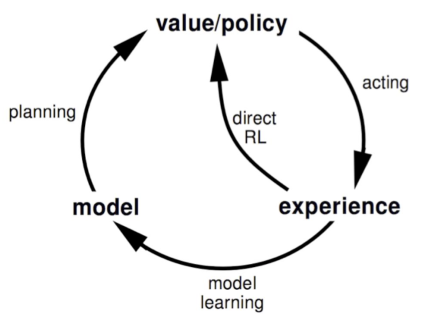
\includegraphics[width=\linewidth]{images/F1.png}
    \label{fig:Scaled Dot Product Attention}
    \vspace{-10pt}
\end{wrapfigure}
The \textbf{Dyna} architecture directly integrates learning and planning.

The agent:
\begin{compactitemize}
    \item uses real experience to update both the model and the value function (or policy);
    \item uses the model to generate simulated experience;
    \item applies model-free algorithms both to real data and to simulated data.
\end{compactitemize}

In this way:
\begin{compactitemize}
    \item real experience keeps contact with the true MDP;
    \item simulated experience speeds up learning;
    \item learning and planning take place continuously, not in separate phases.
\end{compactitemize}

Dyna therefore represents an elegant compromise between Model-Free and Model-Based RL,
and it is the basis of many modern architectures that integrate simulation, learning and real-time decision making.
\begin{figure}[H]
    \centering
    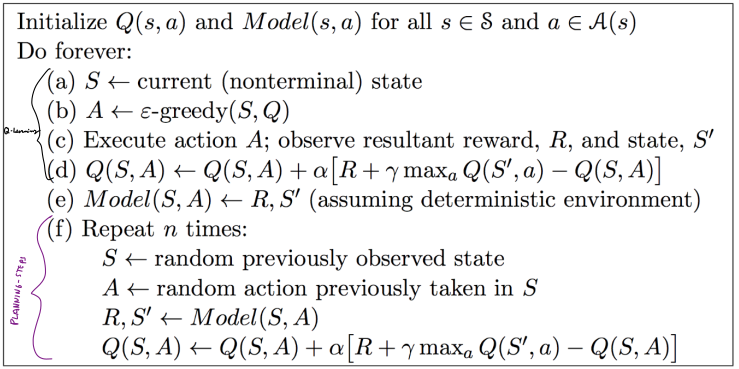
\includegraphics[width=0.8\textwidth]{images/F2.png}
    \label{fig:student_markov_chain}
\end{figure}


\section{Simulation-Based Search}

In the context of model-based RL we can use the model not to solve the whole MDP,
but only to decide which action to take \emph{now}, in the current state $s_t$.
This idea is called \textbf{simulation-based search}.

The principle is the following: instead of interacting with the real environment, we generate
fictitious episodes using the model $\mathcal{M}_\nu$ and a simulation policy $\pi$.
From these simulated episodes we estimate the values of the actions and choose the best one.

Formally, starting from $s_t$ we simulate $K$ episodes:
\[
\bigl\{\, s_t^k, A_t^k, R_{t+1}^k, \dots, S_T^k \,\bigr\}_{k=1}^K
\sim \mathcal{M}_\nu, \pi.
\]

On these $K$ episodes we can apply \emph{model-free} algorithms exactly as
if they were real experience. In practice:

\begin{compactitemize}
    \item if we apply \textbf{Monte Carlo control} to the simulated episodes we obtain
          a \emph{Monte Carlo search};
    \item if we apply \textbf{Sarsa} (or other TD methods) we obtain a form of
          \emph{TD search}.
\end{compactitemize}

So: the model is used only to generate trajectories, while the value update
remains the classic one of model-free RL.

\subsection{Simple Monte Carlo Search}

\textbf{Simple Monte Carlo Search} is the most direct version of this idea.

Suppose we have:
\begin{compactitemize}
    \item a model $\mathcal{M}_\nu$;
    \item a simulation policy $\pi$.
\end{compactitemize}

We are in the real state $s_t$ and we must choose the action $a_t$.

For \emph{each} possible action $a \in \mathcal{A}$:

\begin{enumerate}
    \item we fix the first action to $a$ and simulate $K$ episodes from the model:
    \[
    \bigl\{\, s_t^k, a, R_{t+1}^k, S_{t+1}^k, A_{t+1}^k, \dots, S_T^k \,\bigr\}_{k=1}^K
    \sim \mathcal{M}_\nu, \pi.
    \]
    The complete history of each episode is sampled jointly from the model
    (for transitions and rewards) and from the policy $\pi$ (for future actions).

    \item for each episode we compute the return starting from $t$:
    \[
    G_t^k = R_{t+1}^k + \gamma R_{t+2}^k + \dots + \gamma^{T_k - t - 1} R_{T_k}^k.
    \]

    \item we estimate the value of $a$ in $s_t$ by averaging the returns:
    \[
    Q(s_t,a)
    =
    \frac{1}{K} \sum_{k=1}^{K} G_t^k
    \;\approx\;
    q^\pi(s_t,a).
    \]
\end{enumerate}

Finally we choose the real action that maximizes this estimate:
\[
a_t = \arg\max_{a \in \mathcal{A}} Q(s_t,a).
\]

Important observations:

\begin{compactitemize}
    \item only the actions in the \emph{root state} $s_t$ are evaluated;
    \item the successor states are neither stored nor reused: each decision
          starts again from scratch at the next time-step.
\end{compactitemize}

\subsection{Monte Carlo Tree Search}

\textbf{Monte Carlo Tree Search (MCTS)} extends Simple Monte Carlo Search
by explicitly building a search tree and reusing the information
about all the visited states, not only about the root.

\subsubsection{Evaluation with MCTS}

Given a model $\mathcal{M}_\nu$ and a simulation policy $\pi$, we start from the
real state $s_t$ and once again simulate $K$ episodes:

\[
\bigl\{\, s_t^k, A_t^k, R_{t+1}^k, S_{t+1}^k, A_{t+1}^k, \dots, S_T^k \,\bigr\}_{k=1}^K
\sim \mathcal{M}_\nu, \pi.
\]

During these simulations:
\begin{compactitemize}
    \item we build a tree that contains all the visited states and actions;
    \item for each pair $(s,a)$ we count how many times it has been seen:
          $N(s,a)$;
    \item for each visit we accumulate the return $G_u^k$ starting from the time $u$
          at which the pair $(S_u^k, A_u^k)$ is equal to $(s,a)$.
\end{compactitemize}

The estimated value of $(s,a)$ is therefore:

\[
Q(s,a)
=
\frac{1}{N(s,a)}
\sum_{k=1}^{K}
\sum_{u=t}^{T_k}
\mathbf{1}\bigl( S_u^k = s,\, A_u^k = a \bigr)\, G_u^k
\;\approx\;
q^\pi(s,a).
\]

When the search ends, the real action to execute is the one that maximizes
$Q(s,a)$ in the root state:
\[
a_t = \arg\max_{a \in \mathcal{A}} Q(s_t,a).
\]

Unlike Simple Monte Carlo Search, here we reuse the simulated data to
evaluate \emph{all} the states of the subtree, not only the initial state.

\subsection{Simulation and policy improvement}

In MCTS the simulation policy $\pi$ is not fixed: it improves as
simulations accumulate. Each simulation is conceptually divided into two phases:

\begin{compactitemize}
    \item \textbf{in-tree phase}: as long as we are in nodes already present in the tree,
          the action is chosen with a \emph{tree policy} (for example $\epsilon$-greedy
          on $Q(s,a)$), which balances exploration and exploitation;
    \item \textbf{out-of-tree phase}: when we reach a new state, the tree is
          expanded and from there on a simpler \emph{default policy} is followed,
          typically random.
\end{compactitemize}

After each simulated episode, the values $Q(s,a)$ are updated with Monte Carlo
evaluation and the tree policy is gradually made more greedy with respect to these values.
In practice we are applying \textbf{Monte Carlo control} to the experience
generated by the model; under suitable conditions the estimates converge to:
\[
Q(S,A) \longrightarrow q^*(S,A)
\]
on the explored tree.

In summary:
\begin{compactitemize}
    \item Simple Monte Carlo Search evaluates only the actions in the current state;
    \item Monte Carlo Tree Search builds and updates an entire search tree,
          reusing the same simulated experience for many states and actions.
\end{compactitemize}
\begin{figure}[H]
    \centering
    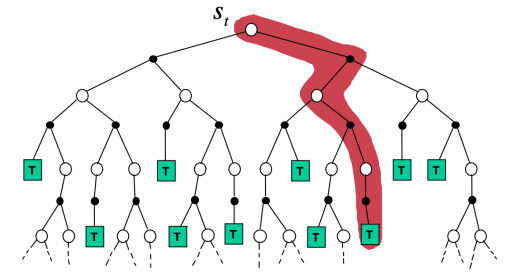
\includegraphics[width=0.8\textwidth]{images/F3.png}
    \label{fig:student_markov_chain}
\end{figure}
\chapter{Exploration and Exploitation}
L'online decision-making comprende due scelte fondamentali, che sono:
\begin{compactitemize}
    \item \textbf{Exploitation}: prendere la migliore decisione utilizzando le informazioni correnti.
    \item \textbf{Exploration}: raccogliere più informazioni
\end{compactitemize}
Tipicamente le soluzioni migliori a lungo termine si trovano sacrificando qualcosa nel breve termine, cioè si preferisce non ottenere tutto subito per avere di più in futuro.

Noi vedremo due approcci per esplorare, che sono:
\begin{compactitemize}
    \item \textbf{Random Exploration}: che consiste nel prendere delle decisioni in maniera randomica, o aggiungere rumore alla greedy policy.
    \item \textbf{Optimism in the face of the uncertainty}: essenzialemente qua calcoliamo l'incertezza delle azioni e prendiamo quella con più incertezza, questo perchè visto che non conosciamo a cosa porta la scelta di quell'azione la esplortiamo sperando porti ad una soluzione migliore. Quindi a differenza di prende l'azione viene presa secono una qaulche base.
\end{compactitemize}

Esistono due modi principali per effettuare un'esplorazione sistematica:

\begin{compactitemize}
    \item \textbf{State/Action Exploration}: consiste nell'esplorare sistematicamente lo spazio degli stati e delle azioni.  
    Ad esempio, ogni volta che uno stato $S$ viene visitato, si seleziona un'azione $A$ diversa per coprire lo spazio delle possibilità.

    \item \textbf{Parameter Exploration}: la policy viene parametrizzata come $\pi(A \mid S, \mathbf{w})$.  
    L'esplorazione viene eseguita provando differenti configurazioni dei parametri $\mathbf{w}$ per un certo periodo di tempo.
    \begin{compactitemize}
        \item \textbf{Vantaggio}: esplorazione coerente.
        \item \textbf{Svantaggio}: non tiene conto direttamente dello spazio stato/azione.
    \end{compactitemize}
\end{compactitemize}

Nel seguito ci concentreremo sull'esplorazione \textbf{stato-azione}.

\section{Multi-Armed Bandit}
Il problema del \emph{multi-armed bandit} è uno dei modelli fondamentali nel Reinforcement Learning, poiché cattura in modo essenziale il dilemma tra esplorazione e sfruttamento. Un bandit è definito come una tupla $\langle \mathcal{A}, \mathcal{R} \rangle$, dove $\mathcal{A}$ è un insieme noto di $m$ azioni, spesso chiamate ``braccia'' della slot machine, mentre $\mathcal{R}^a(r) = \mathbb{P}[R=r \mid A=a]$ rappresenta una distribuzione di probabilità sconosciuta sui possibili reward associati a ciascuna azione $a$.

Ad ogni istante temporale $t$, l'agente seleziona un'azione $a_t \in \mathcal{A}$ e l'ambiente genera un reward $r_t \sim \mathcal{R}_{a_t}$. Poiché le distribuzioni dei reward non sono note in anticipo, l'obiettivo dell'agente è quello di imparare a stimare quali azioni abbiano in media un ritorno più elevato, così da massimizzare la somma cumulata dei reward ricevuti:
\[
\sum_{\tau=1}^t r_\tau .
\]

Per caratterizzare il comportamento delle azioni, si definisce il \emph{valore} di un'azione $a$ come il suo reward atteso:
\[
Q(a) = \mathbb{E}[r \mid a].
\]
Tra tutte le azioni, esiste una scelta ottimale $a^*$ con valore massimo, e il corrispondente valore ottimale è:
\[
V^* = Q(a^*) = \max_{a \in \mathcal{A}} Q(a).
\]

Poiché l'agente non conosce i valori delle azioni, ogni decisione comporta un potenziale costo di opportunità. Questo costo è formalizzato attraverso il concetto di \emph{regret}. Il regret istantaneo è definito come:
\[
l_t = \mathbb{E}\!\left[ V^* - Q(a_t) \right],
\]
ossia la perdita attesa dovuta al fatto che l'azione selezionata non è necessariamente quella ottimale. La somma nel tempo dei regret istantanei definisce il regret totale:
\[
L_t = \mathbb{E}\!\left[ \sum_{\tau=1}^t \left( V^* - Q(a_\tau) \right) \right].
\]
Massimizzare il reward cumulato equivale quindi a minimizzare il regret totale.

Il regret può essere analizzato anche in funzione delle scelte effettuate. Se indichiamo con $N_t(a)$ il numero di volte in cui l'azione $a$ è stata selezionata fino al tempo $t$, e introduciamo per ogni azione $a$ il \emph{gap}:
\[
\Delta_a = V^* - Q(a),
\]
allora il regret totale può essere riscritto come:
\[
L_t = \sum_{a \in \mathcal{A}} \mathbb{E}[N_t(a)] \, \Delta_a.
\]
Questa forma mostra chiaramente come il regret dipenda da quante volte vengono selezionate azioni sub-ottimali (quelle con $\Delta_a > 0$). Un buon algoritmo deve quindi riuscire a mantenere basso il numero di selezioni di azioni con gap elevato. Tuttavia, i gap $\Delta_a$ non sono noti a priori, quindi un algoritmo efficace deve bilanciare esplorazione delle azioni poco conosciute e sfruttamento di quelle che sembrano migliori.
\begin{wrapfigure}{r}{0.5\textwidth}
    \centering
    \vspace{-10pt}
    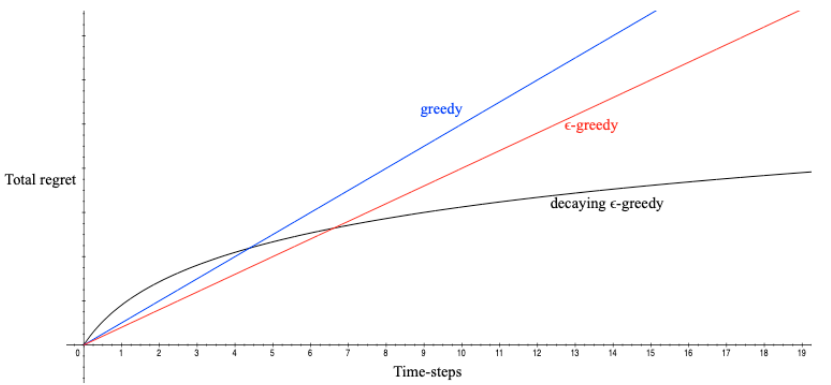
\includegraphics[width=\linewidth]{images/A1.png}
    \label{fig:Scaled Dot Product Attention}
    \vspace{-10pt}
\end{wrapfigure}
Infine, è importante osservare che né un'esplorazione infinita né un completo abbandono dell'esplorazione portano a buone prestazioni. Un algoritmo che continua ad esplorare per sempre accumulerà un regret lineare nel tempo, mentre un algoritmo che non esplora affatto rischia di convergere su un'azione sub-ottimale, anch'esso con regret lineare. Il punto cruciale del problema del multi-armed bandit è proprio determinare se e come sia possibile ottenere un regret sublineare nel tempo, cioè crescere più lentamente di $t$, dimostrando così che l'agente impara effettivamente a comportarsi in modo vicino all'ottimo.

\subsection{Greedy Algorithm}

Per affrontare il problema del multi-armed bandit, una prima classe di algoritmi consiste nello stimare il valore di ciascuna azione mediante valutazione Monte Carlo. L'idea è quella di costruire una stima $\hat{Q}_t(a)$ del valore reale $Q(a)$ a partire dai reward osservati. Per ogni azione $a$, la stima viene aggiornata come media dei reward ottenuti ogni volta che tale azione è stata selezionata. Formalmente, se indichiamo con $N_t(a)$ il numero di volte in cui l'azione $a$ è stata scelta entro il tempo $t$, allora la stima Monte Carlo è:
\[
\hat{Q}_t(a) = \frac{1}{N_t(a)} \sum_{\tau = 1}^{t} r_{\tau} \, \mathbf{1}(a_\tau = a),
\]
dove $\mathbf{1}(\cdot)$ è la funzione indicatrice che vale $1$ quando l'azione al tempo $\tau$ coincide con $a$ e $0$ altrimenti.

Sulla base di questa stima, l'algoritmo \emph{greedy} sceglie semplicemente l'azione che al tempo $t$ presenta il valore stimato più alto. In altre parole, l'azione selezionata è:
\[
a_t^* = \arg\max_{a \in \mathcal{A}} \hat{Q}_t(a).
\]
Questo approccio sfrutta sempre l'informazione disponibile al meglio, scegliendo l'azione che sembra la migliore sulla base dei dati raccolti finora. Tuttavia, il comportamento greedy presenta un limite cruciale: se inizialmente un'azione sub-ottimale riceve per caso reward leggermente migliori, lo stimatore potrebbe sovrastimarne il valore, inducendo l'agente a selezionarla ripetutamente. In questo modo l'algoritmo può ``bloccarsi'' su un'azione non ottimale, senza esplorare sufficientemente le alternative.

L'algortimo greedy ha un total regret \textbf{lineare.}

\subsection{Optimistic Initialization}
Un modo semplice per favorire l'esplorazione è inizializzare le stime dei valori delle azioni a un valore molto alto, tipicamente $\hat{Q}_t(a) = r_{\max}$ per ogni azione $a$. Con tutte le azioni inizialmente valutate come ottimali, l'agente, pur agendo in modo greedy,
\[
a_t = \arg\max_a \hat{Q}_t(a),
\]
finisce per esplorarle tutte almeno una volta.

Tuttavia, questa spinta all'esplorazione è solo iniziale: man mano che le stime vengono aggiornate, i valori $\hat{Q}_t(a)$ scendono verso le loro medie reali e l'algoritmo diventa rapidamente equivalente a un greedy puro, senza più alcun meccanismo di esplorazione. Di conseguenza, poche osservazioni sfortunate possono far scartare definitivamente un'azione ottimale, e anche l'optimistic initialization porta a un regret totale lineare nel tempo.

\subsection{$\varepsilon$-Greedy e $\varepsilon_t$-Decaying}

Un modo semplice per mantenere l'esplorazione continua nel problema del multi-armed bandit è l'algoritmo $\varepsilon$-greedy. In questo approccio, ad ogni passo l'agente:

\begin{compactitemize}
    \item con probabilità $1-\varepsilon$ seleziona l'azione con valore stimato più alto,
    \[
    a = \arg\max_{a \in \mathcal{A}} \hat{Q}_t(a),
    \]
    \item con probabilità $\varepsilon$ sceglie un'azione a caso tra tutte le possibili.
\end{compactitemize}

In questo modo, l'algoritmo continua a esplorare indefinitamente. La scelta di un $\varepsilon$ costante garantisce che il regret istantaneo abbia un limite inferiore:
\[
l_t \ge \frac{\varepsilon}{|\mathcal{A}|} \sum_{a \in \mathcal{A}} \Delta_a,
\]
e quindi il regret totale rimane lineare nel tempo.

Per ridurre il regret nel lungo periodo, è possibile utilizzare una versione con $\varepsilon$ decrescente nel tempo, detta $\varepsilon_t$-greedy. In questo caso si sceglie una sequenza $\varepsilon_1, \varepsilon_2, \dots$ decrescente, ad esempio:
\[
\varepsilon_t = \min \left\{ 1, \frac{c|\mathcal{A}|}{d^2 t} \right\}, \quad c>0, \quad d = \min_{a:\Delta_a>0} \Delta_a,
\]
così che all’inizio l’agente esplori molto e poi gradualmente si comporti in modo quasi greedy. Con questa scelta di decrescita, il regret totale asintotico cresce solo in modo logaritmico con il tempo.

Tuttavia, questo schema richiede di conoscere a priori i gap $\Delta_a$, il che non è realistico nella maggior parte dei casi. L’obiettivo rimane quindi trovare algoritmi capaci di garantire un regret sublineare senza conoscenze preliminari sulle differenze di valore tra le azioni.

\subsection{Lower Bound of Regret}

La difficoltà del problema dipende dalla similarità tra l'azione ottimale e le azioni sub-ottimali. Quando due azioni generano reward con distribuzioni molto simili, l'agente deve raccogliere molte osservazioni per distinguerle, e questo porta inevitabilmente ad accumulare regret. Tale similarità è descritta dalla divergenza di Kullback–Leibler tra le distribuzioni dei reward:
\[
KL(R_a \,\|\, R_{a^*}).
\]

Il teorema classico di Lai e Robbins mostra che ogni algoritmo coerente deve subire un regret almeno logaritmico nel tempo. In particolare:
\[
\lim_{t \to \infty} L_t \;\ge\; \log t \sum_{a:\,\Delta_a>0} \frac{\Delta_a}{KL(R_a \,\|\, R_{a^*})}.
\]

Questo limite indica che il costo dell'esplorazione è inevitabile: per distinguere correttamente le azioni, un algoritmo deve selezionare le azioni sub-ottimali un numero di volte che cresce almeno come $\log t$, rendendo impossibile ottenere regret sub-logaritmico.

\subsection{Optimism in the Face of Uncertainty}

Nel contesto del multi-armed bandit, il principio dell'\emph{Optimism in the Face of Uncertainty} stabilisce che, quando dobbiamo scegliere tra più azioni, dovremmo preferire quelle sulle quali abbiamo maggiore incertezza. L'idea è che un'azione poco esplorata potrebbe in realtà avere un valore molto più alto di quanto stimato finora, e quindi vale la pena indagarla meglio.
\begin{figure}[H]
    \centering
    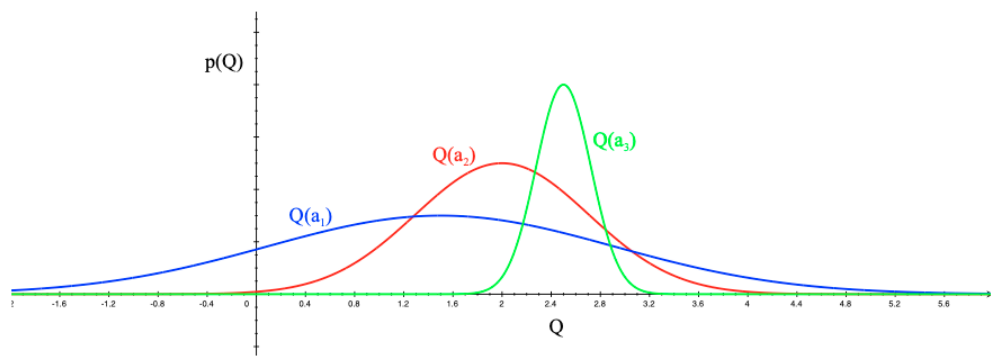
\includegraphics[width=0.6\textwidth]{images/A2.png}
    \label{fig:student_markov_chain}
\end{figure}
Nell'immagine iniziale sono mostrate tre azioni, ciascuna rappresentata da una distribuzione di probabilità sul valore atteso del reward. La curva verde rappresenta un'azione che, secondo le informazioni correnti, sembra avere un valore atteso più alto; la curva rossa un’azione plausibilmente intermedia; mentre quella blu è molto incerta, cioè molto più larga rispetto alle altre. Una distribuzione più larga indica che abbiamo pochi dati su quell'azione, quindi la nostra stima del suo valore è imprecisa.

Il punto centrale dell'approccio ottimistico è proprio questo: un'azione con alta incertezza potrebbe rivelarsi migliore di quanto stimato. Per questo motivo l'algoritmo sceglie di esplorare l'azione blu, nonostante attualmente sembri peggiore di quella verde. Questa scelta “ottimistica” deriva dal considerare non solo il valore atteso stimato, ma anche l’incertezza attorno a tale stima.
\begin{figure}[H]
    \centering
    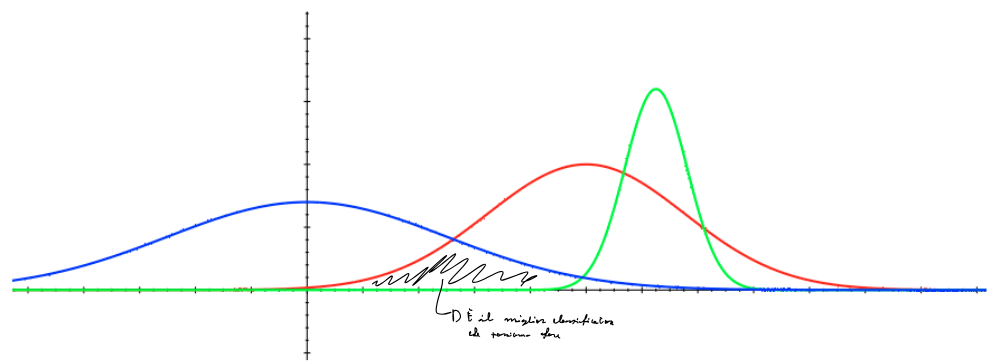
\includegraphics[width=0.6\textwidth]{images/A3.png}
    \label{fig:student_markov_chain}
\end{figure}
Nella seconda immagine vediamo cosa accade dopo aver selezionato l’azione più incerta (la blu). Avendola campionata, la distribuzione si restringe: ora conosciamo meglio il suo valore e quindi siamo meno incerti su di essa. Questa riduzione dell'incertezza elimina la porzione della distribuzione blu che poteva superare le altre, rendendo meno probabile sceglierla nuovamente. Di conseguenza, l’algoritmo inizierà a esplorare altre azioni, come la rossa, continuando questo processo finché non individua l’azione che effettivamente offre il miglior valore atteso.

In sintesi, l’ottimismo di fronte all’incertezza guida l’esplorazione in modo intelligente: selezioniamo le azioni non solo in base alla stima attuale dei loro valori, ma anche in base alla possibilità che queste stime siano troppo conservative. Esplorando sistematicamente le azioni più incerte, l’agente riesce a distinguere meglio tra le diverse distribuzioni di reward e a convergere sull’azione ottimale.

\subsection{Upper Confidence Bounds (UCB)}

L'idea alla base degli \emph{Upper Confidence Bounds} è quella di stimare non solo il valore medio di un'azione, ma anche un intervallo di confidenza entro cui tale valore potrebbe trovarsi. Poiché la nostra stima $Q_t(a)$ è basata su un numero limitato di osservazioni, essa è soggetta a incertezza. Per questo motivo definiamo un termine di confidenza $U_t(a)$ tale che, con alta probabilità,
\[
q(a) \le Q_t(a) + U_t(a).
\]

Questo intervallo dipende fortemente dal numero di volte $N_t(a)$ in cui l'azione $a$ è stata selezionata:
\begin{compactitemize}
    \item se $N_t(a)$ è piccolo, allora $U_t(a)$ è grande: significa che conosciamo poco l'azione e la stima è molto incerta;
    \item se $N_t(a)$ è grande, allora $U_t(a)$ è piccolo: la nostra stima di $Q_t(a)$ è più affidabile.
\end{compactitemize}

Seguendo il principio dell'ottimismo nell'incertezza, l'agente seleziona l'azione che massimizza la somma tra valore stimato e banda di confidenza:
\[
a_t = \arg\max_a \left( Q_t(a) + U_t(a) \right).
\]

Questo permette di bilanciare automaticamente esplorazione e sfruttamento: le azioni meno esplorate avranno $U_t(a)$ maggiore e quindi verranno selezionate più spesso.

\subsection{Hoeffding's Inequality}

Per costruire concretamente il termine di confidenza $U_t(a)$ utilizziamo la disuguaglianza di Hoeffding. Siano $X_1, \dots, X_t$ variabili i.i.d.\ in $[0,1]$ e sia
\[
\bar{X}_t = \frac{1}{t} \sum_{\tau=1}^t X_\tau
\]
la media campionaria. Hoeffding garantisce che
\[
\mathbb{P}\!\left( \mathbb{E}[X] > \bar{X}_t + u \right) \le e^{-2tu^2},
\]
cioè la probabilità che il valore atteso superi la stima empirica più $u$ decresce esponenzialmente con il numero di osservazioni.

Applicando questa disuguaglianza al reward di un'azione $a$ condizionato sulla selezione di tale azione otteniamo:
\[
\mathbb{P}\!\left( q(a) > Q_t(a) + U_t(a) \right)
\le e^{-2 N_t(a)\, U_t(a)^2}.
\]

Questa è l’intuizione matematica che ci permette di costruire una banda di confidenza in modo rigoroso.

\subsection{Calcolo della Banda di Confidenza}

Per calcolare $U_t(a)$ scegliamo una probabilità $p$ che rappresenti il rischio che il valore reale superi la banda di confidenza. Impostiamo:
\[
e^{-2 N_t(a)\, U_t(a)^2} = p.
\]

Risolviamo rispetto a $U_t(a)$:
\[
U_t(a) = \sqrt{\frac{-\log p}{2N_t(a)}}.
\]

Possiamo far variare $p$ nel tempo, ad esempio ponendolo come funzione $p=f(t)$ che diminuisce all'aumentare del numero di osservazioni. In questo modo, man mano che raccogliamo dati, l'intervallo di confidenza si restringe e l'algoritmo converge verso l'azione ottimale.

\subsection{UCB1}

Utilizzando come scelta $p = t^{-4}$ otteniamo una forma particolarmente semplice ed efficace, che dà origine all'algoritmo \textbf{UCB1}. In questo caso la banda di confidenza diventa:
\[
U_t(a) = \sqrt{\frac{2\log t}{N_t(a)}},
\]
e la regola di selezione delle azioni risulta:
\[
a_t = \arg\max_a \left[ Q_t(a) + \sqrt{\frac{2\log t}{N_t(a)}} \right].
\]

L'algoritmo UCB1 garantisce un regret totale asintotico logaritmico:
\[
\lim_{t \to \infty} L_t \le 
8 \log t \sum_{a : \Delta_a > 0} \frac{1}{\Delta_a}.
\]

Questo risultato è notevole perché raggiunge (a costanti moltiplicative) il lower bound di Lai e Robbins, rendendo UCB uno degli algoritmi ottimali per il problema del multi-armed bandit.

\subsection{Bayesian Bandits}

Finora non abbiamo fatto alcuna assunzione sulla forma delle distribuzioni di reward. I \emph{Bayesian bandits}, invece, sfruttano conoscenza a priori sulle distribuzioni dei reward.  
L’idea è quella di modellare il valore delle azioni tramite un insieme di parametri $\mathbf{w}$, ad esempio assumendo che ogni azione abbia una distribuzione gaussiana indipendente con media e varianza ignote:
\[
\mathbf{w} = [\mu_1, \sigma_1^2, \dots, \mu_k, \sigma_k^2].
\]

A partire da un prior $p(\mathbf{w})$ e dai reward osservati, possiamo calcolare la distribuzione a posteriori al tempo $t$:
\[
p(Q(a)\mid h_t) = p(Q(a)\mid \mathbf{w})\, p(\mathbf{w} \mid h_t),
\]
dove $h_t$ rappresenta la storia delle osservazioni fino al tempo $t$.

La conoscenza a posteriori viene poi utilizzata per guidare l’esplorazione. Due metodi molto comuni sono:

\begin{compactitemize}
    \item \textbf{Bayesian UCB}: utilizza la distribuzione a posteriori per costruire una stima ottimistica del valore;
    \item \textbf{Probability Matching}: seleziona un’azione in proporzione alla probabilità che sia ottimale.
\end{compactitemize}

Se il prior è accurato, i Bayesian bandits possono ottenere prestazioni migliori rispetto ai metodi frequentisti.

\begin{figure}[H]
    \centering
    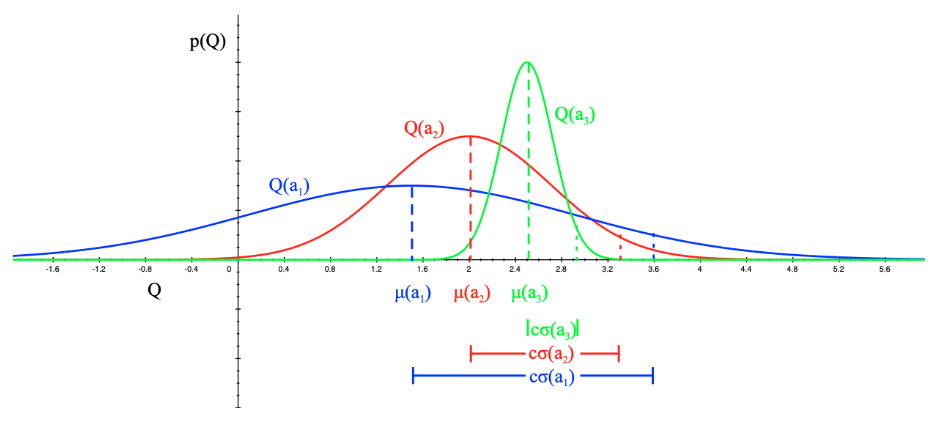
\includegraphics[width=0.8\textwidth]{images/A4.png}
    \label{fig:student_markov_chain}
\end{figure}
\subsection{Bayesian UCB}

Consideriamo il caso in cui le distribuzioni dei reward siano gaussiane:
\[
R_a(r) = \mathcal{N}(r; \mu_a, \sigma_a^2).
\]

Utilizzando la legge di Bayes, possiamo calcolare la distribuzione a posteriori sui parametri $\mu_a$ e $\sigma_a^2$ combinando il prior con i reward osservati. La distribuzione a posteriori del valore di un’azione $a$ ha quindi una deviazione standard $\sigma_a$ che misura l’incertezza residua.

L’idea del \emph{Bayesian UCB} è quella di costruire un limite superiore di confidenza direttamente dalla posterior:
\[
U_t(a) = c\, \sigma_a,
\]
dove $c$ è un parametro che controlla quanto essere “ottimisti”.

L’azione selezionata è quindi:
\[
a_t = \arg\max_a \left( Q_t(a) + c\, \sigma_a \right).
\]

In questo modo, un’azione molto incerta (varianza alta) riceve un aumento maggiore del proprio valore stimato e viene scelta più spesso, coerentemente con il principio dell’ottimismo nell’incertezza.

\subsection{Probability Matching}

Il \emph{Probability Matching} seleziona l’azione $a$ in proporzione alla probabilità che essa sia realmente l’azione ottimale. Formalmente:
\[
\pi(a) = \mathbb{P}\!\left( Q(a) = \max_{a'} Q(a') \,\middle|\, R_1, \dots, R_{t-1} \right).
\]

Questo metodo è naturalmente ottimista: se un’azione è molto incerta, la posterior assegna una probabilità non trascurabile che possa essere la migliore, e quindi quell’azione verrà selezionata più spesso. Tuttavia, calcolare esattamente queste probabilità può essere difficile in modo analitico.

\subsection{Thompson Sampling}

Il \emph{Thompson Sampling} è una versione campionata del probability matching. L’idea è molto semplice:

\begin{enumerate}
    \item Si calcola la distribuzione a posteriori $p(\mathbf{w}\mid R_1,\dots,R_{t-1})$ tramite la legge di Bayes.
    \item Si estrae un campione di una funzione valore $Q(a)$ dalla posterior.
    \item Si seleziona l’azione con il valore più alto nel campione:
    \[
    a_t = \arg\max_a Q(a).
    \]
\end{enumerate}

Ripetendo questo schema a ogni passo, la probabilità di selezionare un’azione coincide con la probabilità che essa sia ottimale secondo il posterior: questo realizza esattamente il probability matching in modo semplice ed efficiente.

Un risultato fondamentale è che il Thompson Sampling raggiunge il lower bound di Lai e Robbins nei bandit di tipo Bernoulli, risultando quindi ottimalmente efficiente dal punto di vista del regret asintotico.


\chapter{Simulation Modeling}
In this chapter we will answer four fundamental questions, which are:
\begin{compactitemize}
    \item What is \textbf{Simulation}?
    \item What is a \textbf{System}?
    \item What is a \textbf{Model}?
    \item What is a \textbf{Discrete-Event} Simulation?
\end{compactitemize}

\section{What is Simulation?}

\textbf{Simulation} can be defined, in a very general sense, as the process of designing a model of a real system and conducting experiments on that model with the goal of:
\begin{compactitemize}
    \item understanding the behaviour of the system over time;
    \item evaluating different strategies for the operation of the system.
\end{compactitemize}

\begin{wrapfigure}{r}{0.5\textwidth}
    \centering
    \vspace{-10pt}
    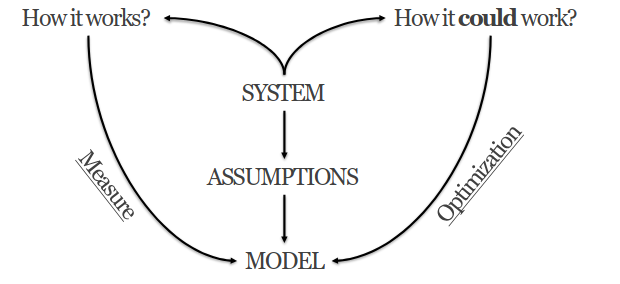
\includegraphics[width=\linewidth]{images/L2.png}
    \label{fig:Scaled Dot Product Attention}
    \vspace{-10pt}
\end{wrapfigure}
This is a deliberately broad, high-level definition: the central idea is that, instead of intervening directly on the real system, a simplified representation of it is built and the effects of decisions are studied in a controlled environment.

More formally, a simulation is the imitation of the operation of a real system along the time axis. It first of all requires the definition of a set of assumptions about the system, then the generation of an \emph{artificial history} of the system itself and finally the observation of that history to draw inferences about the operating characteristics of the system.

\subsection{Objectives of Simulation}

The use of simulation essentially responds to two main objectives.
The first is observing the behaviour of a system as it is, that is, a classic \textbf{AS-IS} analysis. In this case we want to measure performance metrics, identify bottlenecks or understand the internal dynamics of the system.

The second objective is the optimization of the system, in a \textbf{TO-BE} logic. Here simulation is used to answer \emph{what-if} questions: what would happen if we modified a component of the system? If we changed a decision rule? If we introduced a new technology? In this way it is possible to evaluate alternatives without having to implement them in the real world.

\subsection{Simulation as a Process: System, Model, Simulation}

It is fundamental to clarify that simulation is a \textbf{process}, not a single object.
The process follows a very precise conceptual scheme:

\begin{center}
\textbf{System} $\longrightarrow$ \textbf{Model} $\longrightarrow$ \textbf{Simulation}
\end{center}

The \textbf{system} is the real system we want to study, for example a bank, a warehouse or a supply chain.
From the system a \textbf{model} is built, which is nothing but an \emph{approximation} and a \emph{simplification} of the real system. The model does not include everything, but only those aspects that are relevant to the objectives of the study.
Finally, from the model we obtain the \textbf{simulation}, that is, the execution of the model over time to produce artificial data to be analysed.

This point is crucial: \emph{the simulation does not learn anything directly from the real system}, but only from what the model represents. Consequently, the quality of the simulation results depends entirely on the quality of the model.

\subsection{Simulation Techniques}

In some cases the models are simple enough to be analysed with classic mathematical tools, such as probability, differential calculus or mathematical programming. In these situations it is possible to obtain exact analytical solutions.

However, many real systems show a high level of complexity: non-linear behaviours, multiple interactions, random events and temporal dependencies make an analytical solution impossible or impractical. In these cases we resort to simulation models based on computation.

\subsection{When Simulation Is Appropriate}

Simulation is a particularly suitable tool when we want to study the internal operation of a complex system, analyse the effect of organizational or environmental changes, understand how variations of the inputs affect the outputs, verify analytical solutions or support education and training activities.

In all these cases, the main advantage is the possibility of experimenting without risks for the real system.
\begin{figure}[H]
    \centering
    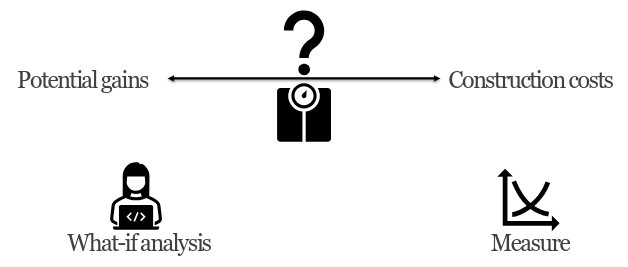
\includegraphics[width=0.6\textwidth]{images/L1.png}
    \label{fig:student_markov_chain}
\end{figure}
\subsection{When Simulation Is \emph{Not} the Appropriate Tool}

It is equally important to understand when \textbf{simulation is not the right tool}. An improper use of simulation can lead to misleading results, waste of resources and wrong decisions.

First of all, simulation is not appropriate when the problem can be easily solved with common sense or with a simple analytical solution. In these cases, building a simulation model would be unnecessarily expensive.

Simulation is not suitable either when carrying out direct experiments on the real system is cheaper, faster or more informative than building a model.

Another important limitation concerns the availability of resources: if there is not enough time, data or expertise, the result will be a poor and unreliable model.

The most critical point, however, is the following: \textbf{if the model is not validated, the simulation is not reliable}.
Simulation works exclusively on the model. If the model does not adequately represent the real system, then the simulation will inevitably produce wrong results. In this case, it does not matter how sophisticated the simulation is or how accurate the analysis is: the conclusions will be wrong because they are based on a wrong representation of the system.

In other words:
\begin{center}
\emph{Invalid model $\Rightarrow$ invalid simulation $\Rightarrow$ invalid decisions}
\end{center}

For this reason, model validation is one of the most delicate and fundamental steps in every simulation study.

Finally, simulation is not appropriate when the level of detail required to answer the questions of interest is so high that it makes the model excessively complex, expensive and difficult to interpret.

\subsection{Advantages and Disadvantages of Simulation}

Among the main advantages of simulation is the possibility of exploring new operating policies without disturbing the real system, testing new designs without committing resources, verifying hypotheses about the behaviour of the system and better understanding the interactions between variables and the bottlenecks.

On the other hand, simulation requires specific expertise, can be expensive in terms of time and computational resources, and produces results that are always estimates or approximations, affected by the variability of the inputs.

\subsection{Areas of Application}

Simulation finds application in numerous contexts, including traffic management, the introduction of new automation technologies, the management of disruptions in demand, supply chain design, last-mile logistics, financial evaluations and optimal control problems.

In all these cases, simulation provides a safe environment in which to experiment and make informed decisions, provided that the model on which it is based is accurately built and validated.

\section{What is a System?}

In order to build a simulation model it is fundamental to first clarify what is meant by \textbf{system}. In general, a system is defined as a set of entities that interact with each other in a regular or interdependent way with the purpose of achieving a certain goal.

This definition highlights three essential elements: the existence of several components, the interaction between these components and the presence of a goal or a function that the system must perform. A system, therefore, is not simply a collection of objects, but an organized structure in which the parts mutually influence the overall behaviour.

A classic example is an industrial production system, such as a car assembly line. In this case, the system is the entire production process; the entities are machines, workers and components; the goal is the production of high-quality vehicles at a certain rate.

\subsection{System, State, and Environment}

The practical meaning of system always depends on the objectives of the simulation study. Depending on what we want to analyse, the way in which the system is delimited changes.

The \textbf{state} of a system is defined as the set of variables needed to describe it at a given instant of time. If the state is known, then the future behaviour of the system can be determined (in a probabilistic or deterministic sense) from it.

The \textbf{environment} includes everything that is external to the system but that can influence its behaviour. The distinction between system and environment is not absolute, but depends on the choices of the modeller and on the purpose of the simulation.

The \textbf{boundary} represents the conceptual border that separates the system from the environment. For example, in a simulation of a bank, the customer arrival process can be considered part of the environment, since it is not under the control of the bank, while the service policy (number of counters, priority rules) is part of the system.

\subsection{Components of a System}

To understand and model a system it is necessary to identify its fundamental components. A first component is the \textbf{entity}, that is, an object of interest within the system, such as a customer, a product or a vehicle.

Each entity is characterized by one or more \textbf{attributes}, which describe its properties. In the case of a banking system, for example, the attributes of a customer can include the account balance, the credit rating or a unique identifier.

An \textbf{activity} represents a period of time during which a specific operation takes place, such as the delivery of a service, a payment or a processing phase. Activities have a duration that can be deterministic or random.

An \textbf{event}, instead, is an instantaneous occurrence that causes a change in the state of the system. The arrival of a customer or the completion of a service are typical examples of events. Events can be exogenous, if they originate from the environment, or endogenous, if they are generated by the system itself.

Finally, the \textbf{state variables} are the minimal set of variables capable of completely describing the state of the system at every instant of time, such as the number of busy servers or the length of a queue.

It is important to underline that there is no universal list of components valid for every system: the choice always depends on the objectives of the simulation study.
\begin{figure}[H]
    \centering
    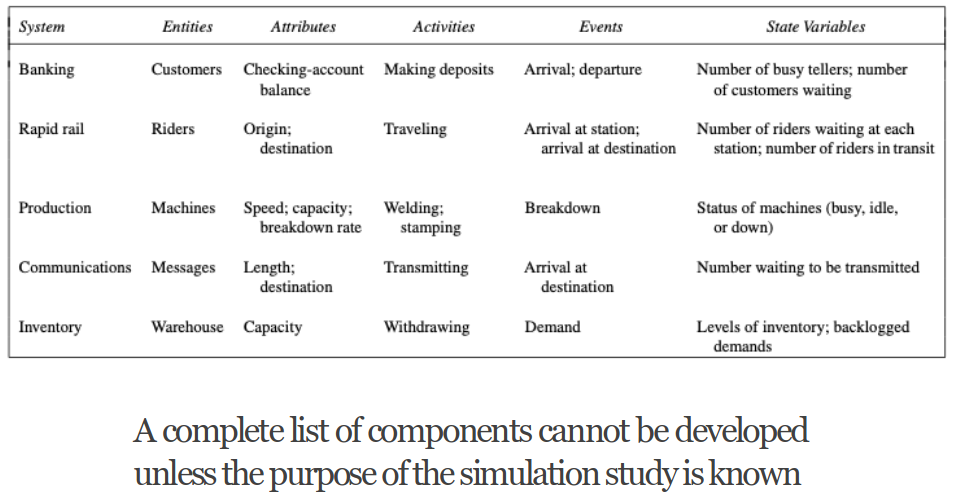
\includegraphics[width=0.8\textwidth]{images/L3.png}
    \label{fig:student_markov_chain}
\end{figure}
\subsection{Discrete and Continuous Systems}

A system is called \textbf{discrete} if its state variables change only at discrete instants of time, typically when events occur. Classic examples are a bank, a warehouse or a production line.

A system is instead \textbf{continuous} if the state variables evolve continuously over time, as in the case of the water level in a dam or the trend of a financial variable.

This distinction is conceptual and does not impose a rigid correspondence between system and model. A continuous system can be approximated through a discrete model and vice versa. The choice depends on the nature of the system and on the purpose of the analysis.

In conclusion, understanding what is meant by system, how to define its boundaries and which components to include is an essential step before building a model and, subsequently, a reliable simulation. A wrong definition of the system inevitably leads to inadequate models and to simulations that are not representative of reality.

\section{What is a Model?}

After having defined what a \textbf{system} is, the next step in the simulation process is the construction of a \textbf{model}. A model is a representation of a system, built with the purpose of studying its behaviour, understanding its internal dynamics or predicting its performance under different decision policies.

By definition, a model is a \textbf{simplification} of the real system. It is neither possible nor desirable to include every detail of the real world: the goal is instead to keep only the elements relevant to the problem being analysed. However, this simplification must be carefully balanced, since the model must be detailed enough to allow valid and reliable conclusions.

In this sense the famous principle of George Box applies: \emph{“All models are wrong, but some are useful”}. Every model is inevitably “wrong” because it does not reproduce reality perfectly, but it can still be extremely useful if it captures the essential aspects of the system that influence the behaviour of interest.

\subsection{Purpose of a Model}

A model is built for a very specific purpose. In some cases the goal is to understand the relations between the components of the system; in other cases we want to predict the performance of the system under new operating conditions or new decision policies.

Although in principle a system could be studied through direct experiments, in practice this approach is often impractical. The system might not exist yet, as in the case of a new production plant, or it might be too expensive, risky or complex to experiment on directly. In these cases, the model becomes the main analysis tool.

It is important to underline that, if the purpose of the study changes, the model must change too. A model built to analyse the waiting times of a system might not be suitable for evaluating energy costs or robustness to failures.

\subsection{Model Complexity and Trade-offs}

Building a model requires a compromise between simplicity and realism. A model that is too simple risks neglecting important variables, leading to misleading conclusions. On the contrary, an excessively complex model can become difficult to understand, implement and validate, paradoxically ending up being as opaque as the real system.

As the level of detail increases, so do the requirements in terms of data, development time and computational costs. For this reason, a good model is not the most complex one possible, but the one that includes only what is necessary to answer the questions posed by the study.

\subsection{Classification of Models}

Models can be classified along several dimensions, depending on their fundamental characteristics.

A first distinction is between \textbf{physical models} and \textbf{mathematical models}. Physical models are tangible, scaled representations of the real system. Mathematical models instead describe the system through logical and quantitative relations, using equations and mathematical symbols. In the context of simulation, we work almost exclusively with mathematical models.

Models can also be \textbf{static} or \textbf{dynamic}. A static model represents the system at a single instant or without a real temporal evolution, as in the case of some Monte Carlo simulations. A dynamic model, instead, explicitly represents the change of the state of the system over time and is the most common type of model in the simulation of real processes.

A further distinction concerns \textbf{deterministic} and \textbf{stochastic} models. In deterministic models there are no random variables and, for the same input, the output is always identical. In stochastic models, instead, some components are random and the outputs are therefore estimates of the true performance of the system.

Finally, models can be \textbf{discrete} or \textbf{continuous}. In discrete models the state of the system changes only at discrete instants of time, while in continuous models the state evolves continuously. There is no rigid correspondence between system and model: a continuous system can be modelled in a discrete way and vice versa, depending on the objectives of the study.

\subsection{Models and Simulation}

In the simulation process, the model occupies a central position. We start from a real system, which is approximated through a model; the model is then used to generate a simulation, that is, an “artificial history” of the system. The conclusions drawn from the simulation depend entirely on the quality of the model.

If the model is not appropriate or not validated, the simulation will produce misleading results. In other words, a simulation can never compensate for a bad model: precise results obtained from a wrong model lead to wrong decisions. For this reason, the construction and validation of the model are among the most critical phases of any simulation study.
\begin{figure}[H]
    \centering
    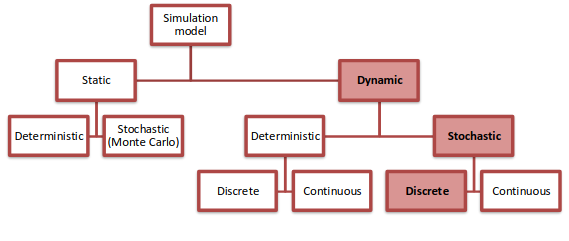
\includegraphics[width=0.8\textwidth]{images/L4.png}
    \label{fig:student_markov_chain}
\end{figure}

\section{What is a Discrete-Event Simulation (D.E.S.)}

A Discrete-Event Simulation (DES) is a specific class of simulation models used to represent systems that evolve over time through the occurrence of discrete events. In this framework, the state of the system does not change continuously, but only at distinct points in time, when specific events occur.

Formally, a discrete-event simulation models a system whose state variables change instantaneously at separate points in time. These points in time are called \emph{events}. Each event corresponds to a meaningful occurrence in the system, such as the arrival of an entity, the start of a service, or the completion of an activity. When an event occurs, the state of the system may change as a consequence.

Unlike analytical models, DES does not aim to solve equations analytically. Instead, it relies on numerical methods and computational procedures. Models are not \emph{solved}, but rather \emph{run}. By executing the simulation model, an artificial history of the system is generated, and observations are collected over simulated time. These observations are then analysed to obtain estimates of the true performance measures of the real system.

\subsection{Example: Single-Server Queue}

To illustrate the concept of discrete-event simulation, consider a simple service system with a single server, such as a one-person barbershop, a bank teller, or an information desk. The objective of the study is to estimate the expected average delay experienced by customers waiting in line. The delay is defined as the time interval between the arrival of a customer and the start of service.

The system is described through a set of state variables, such as the status of the server (idle or busy), the queue length, and the arrival times of customers. The evolution of the system is driven by events. In this example, three types of events are sufficient to fully capture the system dynamics: the \textbf{arrival} of a customer, the \textbf{start of service}, and the \textbf{departure} of a customer, which coincides with the completion of service. Each of these events may modify the system state when it occurs.

This example highlights the key characteristics of DES: state changes occur only at event times, and the system dynamics are fully determined by the sequence and timing of events.
\begin{figure}[H]
    \centering
    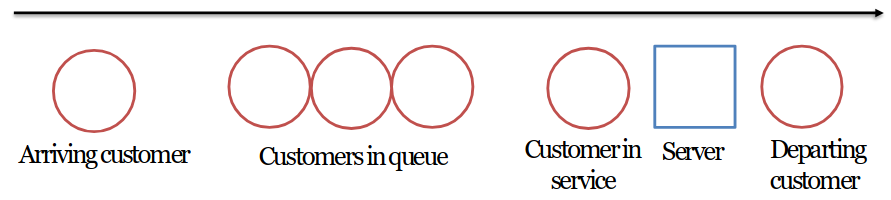
\includegraphics[width=0.8\textwidth]{images/L5.png}
    \label{fig:student_markov_chain}
\end{figure}
\subsection{Steps in a Simulation Study}

A discrete-event simulation study follows a structured process, which can be divided into four main phases: 
\begin{compactitemize}
    \item \textbf{Discovery}
    \item \textbf{Model Building}
    \item \textbf{Run}
    \item \textbf{Implementation}
\end{compactitemize}
The first phase is the discovery and orientation phase. This phase begins with problem formulation. The problem must be clearly understood before any modelling effort starts. A common mistake at this stage is developing a solution without a well-defined problem. Along with problem formulation, the objectives of the study are defined and an overall project plan is established. The objectives specify which questions the simulation is expected to answer, while the project plan addresses practical aspects such as time constraints, costs, and required resources.

The second phase is the model building phase, which is the core of the simulation study. It starts with model conceptualization, where the essential features of the system are identified and translated into a conceptual model. This involves selecting the basic assumptions that characterise the system and deciding which elements are relevant for the study. Model construction is as much an art as it is a science: a common practice is to start with a simple model and progressively introduce complexity, ensuring that each added detail contributes useful information.

\begin{wrapfigure}{r}{0.6\textwidth}
    \centering
    \vspace{-10pt}
    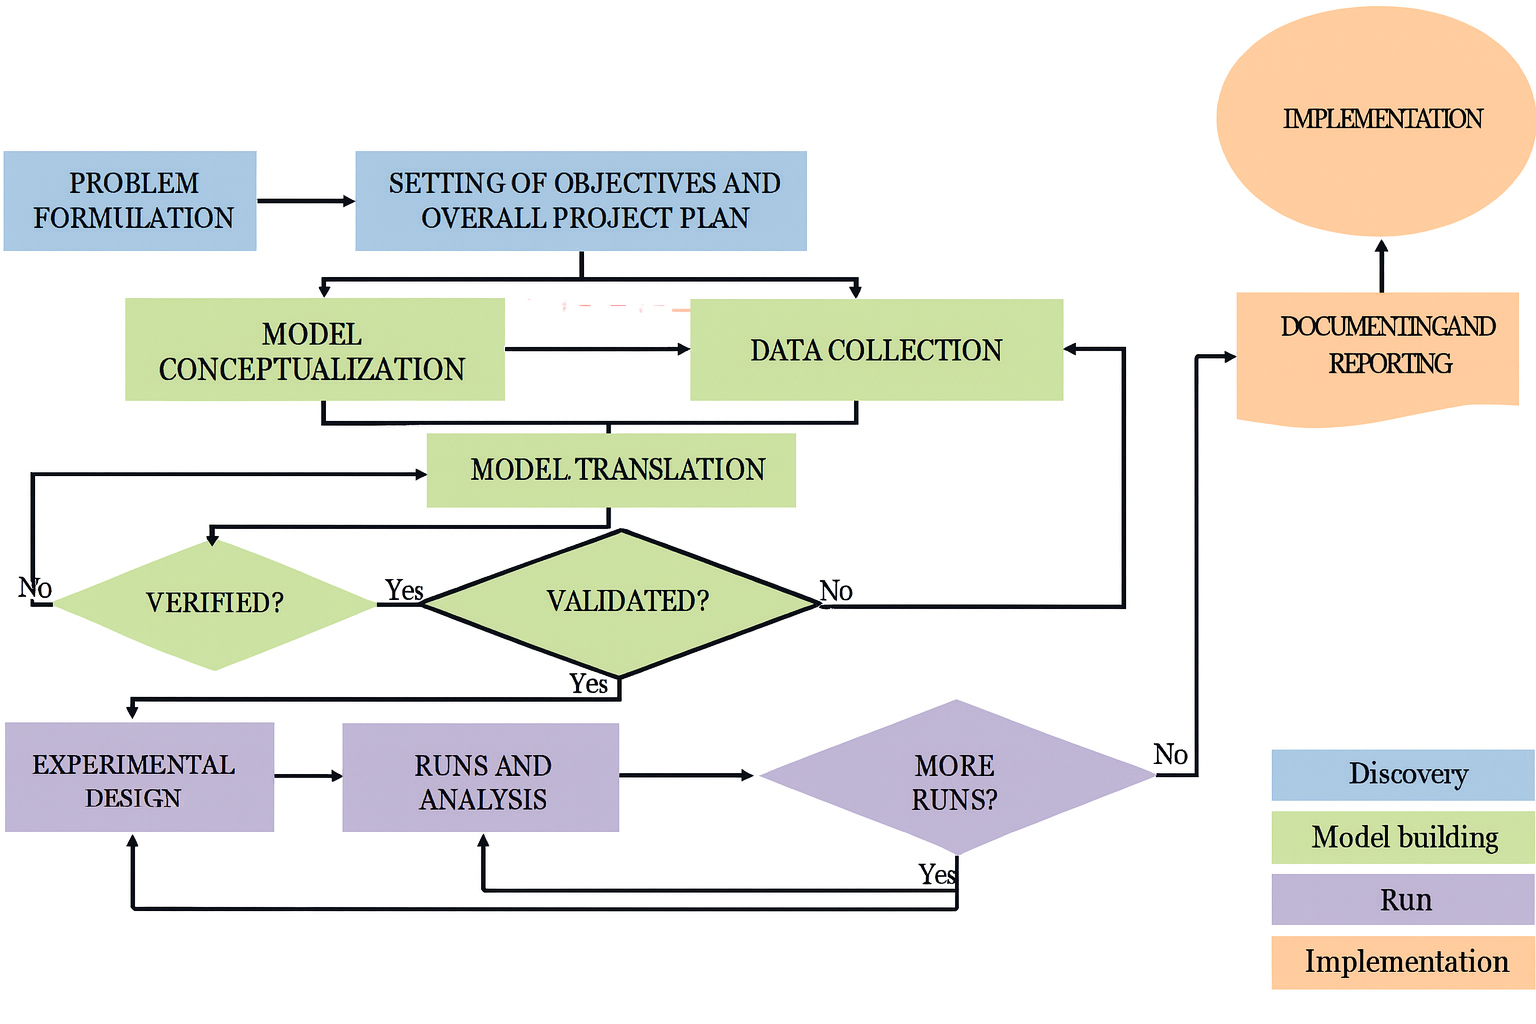
\includegraphics[width=\linewidth]{images/L6.png}
    \label{fig:Scaled Dot Product Attention}
    \vspace{-10pt}
\end{wrapfigure}
Data collection is tightly coupled with model building. As the model evolves, different types and levels of input data may be required. Because data collection can be time-consuming and expensive, it should start early and proceed in parallel with model development. Once the conceptual model and data are available, the model is translated into a software implementation. In this course, this translation is performed using Python and the SimPy library.

A crucial part of the model building phase is verification and validation. Model verification answers the question: “Is the model implemented correctly?” It focuses on whether the code faithfully represents the conceptual model and behaves as intended. Model validation, instead, addresses a deeper question: “Does the model accurately represent the real system?” Validation is achieved through calibration and comparison between simulated outputs and observed system behaviour. Discrepancies are not necessarily failures; they often provide valuable insight into the system and guide improvements to the model. This is the most critical step of the entire simulation process: an invalid model inevitably leads to invalid decisions, regardless of how well the simulation is executed.

The third phase is the run phase. At this stage, the validated model is used to perform experiments. An experimental design is defined, specifying the decision alternatives to be evaluated. For each alternative, key choices must be made, such as the length of the simulation run, the presence and duration of a warm-up period, and the number of independent replications. The objective is to obtain unbiased performance estimates with sufficiently low variance.

The final phase is the implementation phase. This includes documentation and reporting, which ensure that the model and results are understandable, reproducible, and reusable in the future. Clear documentation also supports future modifications and extensions of the model. Implementation refers to the actual adoption of a selected alternative in the real system. The success of this phase depends entirely on the quality of all previous steps: a well-defined problem, a valid model, and a rigorous experimental analysis.

In summary, a discrete-event simulation is a powerful and flexible tool for analysing complex dynamic systems. However, its effectiveness relies on a disciplined modelling process, careful validation, and a clear understanding of the limits and assumptions underlying the model.

\end{document}